\documentclass[print]{dissertation}
\usepackage{graphicx}
\usepackage{color}
\usepackage{amsmath}
\usepackage{amssymb}
\usepackage[normalem]{ulem}
\usepackage{adjustbox}
\usepackage{nicefrac,physics}
\usepackage{caption,subcaption,mwe}
\usepackage{ragged2e}

\renewcommand{\vec}[1]{{\boldsymbol #1}}
\renewcommand{\i}{i}
%\newcommand{\rev}[1]{{\color{red}{#1}}} 
\newcommand{\rev}[1]{{{#1}}} 
\def\nn{\nonumber\\}
% \newcommand{\nn}{\nonumber\\}
\newcommand{\non}{\nonumber\\}

\DeclareMathOperator{\sgn}{sgn}
\newcommand{\cind}[3]{c^{(#1)}_{#2}(#3)}
\newcommand{\cdag}[3]{{c^\dagger}^{(#1)}_{#2}(#3)}
\newcommand{\phind}[3]{\phi^{(#1)}_{#2}(#3)}
\newcommand{\sigmap}{\sigma^\prime}
\newcommand{\taup}{\tau^\prime}

\newcommand{\oemga}{\omega}
\newcommand{\tp}{t^\prime}


\usepackage{url}
\usepackage{pgfplots}
\pgfplotsset{width=7cm,compat=1.8}

\usepackage{graphicx}
\usepackage{color}
\usepackage{amsmath,mathtools}
\usepackage{enumitem}
\usepackage{amssymb}
\usepackage{hyperref}
\usepackage[normalem]{ulem}
\usepackage{adjustbox}
\usepackage{nicefrac,physics}
\usepackage{stackengine}
\usepackage{lipsum}
\usepackage{multirow}
\usepackage{array}
\usepackage{feynmp-auto}
\usepackage{comment}
\usepackage{float}


\definecolor{coolblack}{rgb}{0.0, 0.18, 0.39}
\renewcommand{\baselinestretch}{1.1}



\hyphenation{wij-ze}

	\usepackage{caption}
	\usepackage{booktabs}
	\usepackage{varwidth}
	
	\usepackage[utf8]{inputenc}
	\usepackage[english]{babel}
	%\setlength{\parindent}{4em}
	%\setlength{\parskip}{1em}
	
	
	\newcommand{\etal}{\textit{et al}. }
	\newcommand{\ie}{\textit{i}.\textit{e}. }
	\newcommand{\eg}{\textit{e}.\textit{g}. }
	
	\newcolumntype{M}[1]{>{\centering\arraybackslash}m{#1}}
	\newcolumntype{N}{@{}m{0pt}@{}}
	
	\makeatletter
	\newcommand{\thickhline}{%
		\noalign {\ifnum 0=`}\fi \hrule height 2pt
		\futurelet \reserved@a \@xhline
	}
	\newcolumntype{"}{@{\hskip\tabcolsep\vrule width 1pt\hskip\tabcolsep}}
	\makeatother
	
	\newcommand\blankpage{
		\null
		\thispagestyle{empty}
		\addtocounter{page}{-1}
		\newpage}
	
	
	\def\H{\pazocal{H}}
	\def\DT{\Delta_\varphi}
	\def\C{\pazocal{C}}
	\def\A{\pazocal{A}}
	\def\E{\pazocal{E}}
	\def\S{\pazocal{S}}
	\def\L{\pazocal{L}}
	\def\T{\pazocal{T}}
	\def\G{\pazocal{G}}
	\def\K{\pazocal{K}}
	\def\R{\pazocal{R}}
	\def\F{\pazocal{F}}
	\def\N{\pazocal{N}}
	\def\P{\pazocal{P}}
	\def\D{\pazocal{D}}
	\def\O{\pazocal{O}}
	\def\U{\Upsilon}
	\def\dhg{\delta \hat g}

            

	
	\definecolor{myred}{RGB}{180, 38, 38}
	\definecolor{myblue}{RGB}{25, 145, 198}

	\usepackage{calrsfs}
	\usepackage[pages=some,scale=1,angle=0,opacity=0.7]{background}
	%\newcommand\BackImage[2][scale=1]{%
	%	\BgThispage
	%	\backgroundsetup{
	%		contents={\includegraphics[#1]{#2}}
	%	}
	%}
	
	
	\begin{document}
		\sloppy
		
		%% Specify the title and author of the thesis. This information will be used on
		%% the title page (in title/title.tex) and in the metadata of the final PDF.
		\title[]{Proefschrift Aravindh Swaminathan Shankar} %use for title
		\author{Aravindh Swaminathan}{Shankar}
		
		%% Use Roman numerals for the page numbers of the title pages and table of
		%% contents.
		\frontmatter
		
		%%\newgeometry{hmarginratio=1:1}
%\thispagestyle{empty}

%----------------------------------------------------------------------------------------
%	PACKAGES AND OTHER DOCUMENT CONFIGURATIONS
%----------------------------------------------------------------------------------------

%\documentclass[a4paper, 11pt, oneside]{book} % A4 paper size, default 11pt font size and oneside for equal margins

%\newcommand{\plogo}{\fbox{$\mathcal{PL}$}} % Generic dummy publisher logo

%\usepackage[utf8]{inputenc} % Required for inputting international characters
%\usepackage[T1]{fontenc} % Output font encoding for international characters
%\usepackage{fouriernc} % Use the New Century Schoolbook font

%----------------------------------------------------------------------------------------
%	TITLE PAGE
%----------------------------------------------------------------------------------------

%\begin{document} 
\newgeometry{hmarginratio=1:1}
\thispagestyle{empty}

\begin{titlepage} % Suppresses headers and footers on the title page

	%\centering % Centre everything on the title page
	\begin{center}
	%\scshape % Use small caps for all text on the title page
	
	\vspace*{\baselineskip} % White space at the top of the page
	
	%------------------------------------------------
	%	Title
	%------------------------------------------------
	
%\rule{\textwidth}{1.6pt}\vspace*{-\baselineskip}\vspace*{2pt} % Thick horizontal rule
	%\rule{\textwidth}{0.4pt} % Thin horizontal rule
	
	%\vspace{0\baselineskip} % Whitespace above the title
	
	{\huge Strongly interacting electrons in Sachdev-Ye-Kitaev models  \\ 
            and Twisted Bilayer Graphene\\} % Title
	
	%\vspace{1\baselineskip} % Whitespace below the title
	
	%\rule{\textwidth}{0.4pt}\vspace*{-\baselineskip}\vspace{3.2pt} % Thin horizontal rule
	%\rule{\textwidth}{1.6pt} % Thick horizontal rule
	
	%\vspace{1\baselineskip} % Whitespace after the title block
	
	%------------------------------------------------
	%	Subtitle
	%------------------------------------------------
	
	%A Number of Fascinating and Life-changing Templates Presented in a Clear and Concise Way % Subtitle or further description
	
	\vspace*{4\baselineskip} % Whitespace under the subtitle
	{\Large Proefschrift} 
	%------------------------------------------------
	%	Editor(s)
	%------------------------------------------------
	
	%Edited By
	
	\vspace{6\baselineskip} % Whitespace before the editors
	
    
    % {\large ter verkrijging van \\ de graad van doctor aan de Universiteit Leiden, \\ op gezag van rector magnificus prof.dr.ir. H. Bijl, \\ volgens besluit van het college voor promoties \\ te verdedigen op dinsdag 10 oktober 2023 \\ klokke 13:45 uur} % Editor list
     {\large ter verkrijging van \\ de graad van doctor aan de Universiteit Leiden, \\ op gezag van rector magnificus prof.dr.ir. H. Bijl, \\ volgens besluit van het college voor promoties \\ te verdedigen op dinsdag 7 januari 2025 \\ klokke 13:00  uur}
	
	\vspace{3\baselineskip} % Whitespace below the editor list
	
    {\large door}  % Editor affiliation
    
    \vspace{3\baselineskip} % Whitespace below the editor list
    
	{\Large Aravindh Swaminathan Shankar}
    
    %\vspace{1\baselineskip} % Whitespace below the editor list
    
    {\large Geboren te Chennai, Indi{\"e}\\in 1996}
    
	\vfill % Whitespace between editor names and publisher logo
\end{center}

\clearpage
\thispagestyle{empty}

\medskip
\noindent \textbf{Promotores}:\\
Dr. V. Cheianov\\
Prof.dr. K.E. Schalm 

\bigskip
\noindent \textbf{Promotiecommissie}: \\
Dr. V. Gritsev (Universiteit van Amsterdam)\\
Prof.dr. S. Vandoren (Universiteit Utrecht)\\
Prof.dr. C.W.J. Beenakker \\
Dr. S. Bhattacharya \\
Prof.dr. S.J. van der Molen \\





\vspace{2\bigskipamount}

% \vspace*{\fill}
% \noindent
% Casimir PhD series, Delft-Leiden xxxx\\
% ISBN xxx-xx-xxxx-xxx-x\\

\vspace{5pt}
\noindent
An electronic version of this Thesis can be found at \\ 
\href{https://openaccess.leidenuniv.nl}{https://openaccess.leidenuniv.nl}



\vspace*{\fill}
\noindent
The cover represents two ways in which Hyperbolic geometries play a role in the low energy properties of electrons. The yellow curve represents the fermi surface near a van-Hove singularity and the random colored dots represent the SYK model. The graphics were made using the manim python package.

\clearpage
\thispagestyle{empty}


\end{titlepage}
 %this is the file now called 'title page'
		
		%% The (optional) dedication can be used to thank someone or display a
		%% significant quotation.
		
		%\dedication{\epigraph{
			%	To myself and my family.}
			%{}}
		
		%%%%%%%%%%%          TABLE OF CONTENTS               ###############
		\tableofcontents
		
		% Disable indentation
		\setlength{\parindent}{0pt}
		\setlength{\parskip}{1em}
		
		%\include{preface} %I did not use this one
		
		%% Use Arabic numerals for the page numbers of the chapters.
		\mainmatter
		
		%% Turn on thumb indices.
		
		\newgeometry{
			top=1in,
			bottom=1in,
			outer=1in,
			inner=1in,
		}
		\thumbtrue
		
		
		% \chapter{Introduction}
\label{ch:Intro}
\par
The unifying theme in this thesis is the presence of hidden hyperbolic geometries in strongly interacting systems and their bilayers. 

What is a fermi liquid? and what is a non-fermi liquid 

Consider a scattering diagram: self energy proportional to DoS, van hove points can break fermi liquid theory. cite polchinski, shankar.

\newpage     

\section{Interactions enhanced by van hove singularities}


\section{Graphene and its bilayers}
\label{sec:graphene}
Graphene is a single sheet of carbon atoms arranged in a hexagonal lattice~\cite{neto2009electronic}. Its electronic properties can be described by a simple tight binding model which accounts for electrons hopping between its two sublattices, with its hamiltonian given by
\begin{align}
    H &= -t \sum_{\langle i,j\rangle} a_i^\dagger b_j + h.c ,  
\end{align}
and can be diagonalized in terms of two component wavefunctions 
\begin{align}
    \Psi_i = \mqty(a_i \\ b_i  ) .
\end{align}

\begin{figure}
    \centering
    \includegraphics{}
    \caption{Caption}
    \label{fig:enter-label}
\end{figure}


\section{The Kondo effect}
\section{The Sachdev-Ye-Kitaev model}

\section{Statistical physics}
\label{sec:statPhys}
\textbf{TEMPLATE: ERASE LATER}
\par
The primary goal of statistical physics is an exploration of macroscopic quantities and the calculation thereof. Often, the systems we explore are made up of many degrees of freedom, and solving them exactly is impossible. In order to do this, we will assume that the statistical average over all possible states can replace the time average. 
\par 
One of the main assumptions we make when resorting to statistical calculations instead of fully dynamically solving the system is the principle of \textit{ergodicity}. Ergodicity states that if the system is left to evolve, all accessible states will eventually be realized. This assumption helps us often turn insolvable time integrals into relatively easy and, more importantly, simulation-friendly integrals over the probability distributions of those states. For example, let us say we want to study some volume of gas in a container. At standard temperature and pressure, one liter of oxygen contains around $3\cdot 10^{22}$ oxygen molecules moving around the container. Just writing down equations of motion for all molecules would take a very long time, but no practical conclusion can be drawn even if we manage to do it. Hence we turn to the methods of statistical physics.
\par


\section{This thesis}
In the introduction, we have covered the basic ideas used later in this thesis. We started with introductory topics in thermodynamics and statistical physics, then moved to a basic introduction to Monte Carlo methods and all the required knowledge to understand our physical system's simulation design and analyze the results. The proceeding section was dedicated to the basics of machine learning, deep learning, and appropriate selection of model, loss function, and minimization method. The last section culminated in a synergy of the previously mentioned topics by combining quantum physics, Monte Carlo methods, and neural networks in neural quantum states that we used to find the ground state and its energy of lattice gauge theories.

\subsection{Chapter 1 - The Kondo effect in Twisted bilayer graphene}


\subsection{Chapter 2 - Chaos in the bipartite Sachdev-Ye-Kitaev model}



\subsection{Chapter 3 - Wormholes in the Yukawa-Sachdev-Ye-Kitaev model}


		\chapter{Kondo effect in Twisted Bilayer graphene}
\label{ch:KondoTBG}

\section*{Attribution}
This paper has been previously published in Physical Review B, under the title \textbf{\textit{Kondo effect in twisted bilayer graphene}}, together with Dmytro O. Oriekhov, Andrew K. Mitchell and Lars Fritz~\cite{shankar2023kondo}.

\section*{Abstract}
\noindent The emergence of flat bands in twisted bilayer graphene at the magic angle can be understood in terms of a vanishing Fermi velocity of the Dirac cone. This is associated with van Hove singularities approaching the Fermi energy and becoming higher-order. In the density of states this is reflected by flanking logarithmic van Hove divergences pinching off the central Dirac cone in energy space. The low-energy pseudogap of the Dirac cone away from the magic angle is replaced by a power-law divergence due to the higher-order van Hove singularity at the magic angle.
This plays an important role in the exotic phenomena observed in this material, such as superconductivity and magnetism, by amplifying electronic correlation effects.
Here we investigate one such correlation effect -- the Kondo effect due to a magnetic impurity embedded in twisted bilayer graphene. We use the Bistritzer-MacDonald model to extract the low-energy density of states of the material as a function of twist angle, and study the resulting quantum impurity physics using perturbative and numerical renormalization group methods. Although at zero temperature the impurity is only Kondo screened precisely at the magic angle, we find highly nontrivial behavior at finite temperatures relevant to experiment, due to the complex interplay between Dirac, van Hove, and Kondo physics.

\section{Introduction}

The properties of two-dimensional monolayer systems are strongly modified by stacking two layers with a relative twist, the so-called moir\'e effect in twisted bilayer systems~\cite{LopesdosSantos2007PRL}. In particular, twisted bilayer graphene (TBG) exhibits peculiar properties at specific `magic' twist angles~\cite{Suarez2011,Bistritzer2011,Kim2017,Liu2019,Yuan2019,Song2019,Tarnopolsky2019,Cao2018,Caocorrelated2018,Lu2019}. One characteristic of the system at these magic angles is that the non-interacting band structure contains almost-flat bands. This leads to a dramatic enhancement of the density of states (DoS). Consequently, electronic interaction effects are boosted, favoring the appearance of magnetism and other correlated phases, for example superconductivity~\cite{Cao2018,Caocorrelated2018,Lu2019,Ojajarvi2018,Isobe2018,Wu2018,Peltonen2018,Kozii2019,Yankowitz2019,Hazra2019,Hu2019,Xie2020,Julku2020}. 
Away from the magic angle in TBG, the slightly modified Dirac cones of the single layers persist~\cite{LopesdosSantos2007PRL}, giving a low-energy linear pseudogap DoS. However, pronounced van Hove singularities~\cite{vanHove1953} (vHs's) dominate the band structure at higher energies, leading to logarithmic divergences in the DoS. Experimentally, it was recently shown~\cite{Li2010} that as the magic angle is approached, the vHs divergences in the DoS move to lower energy, pinching off the Dirac cone from either side in energy space. At the magic angle, the vHs divergences in the DoS merge, and a single higher-order vHs \cite{Yuan2019} (HO-vHs) emerges, yielding a stronger, power-law divergent DoS. This is a characteristic feature of the emergent flat bands in this system. The enhanced effect of electron correlations due to the HO-vHs in the bulk TBG material has been studied theoretically~\cite{Caocorrelated2018,Lu2019,Isobe2018,Classen2020PRB} and confirmed in scanning tunnelling spectroscopy (STS) experiments~\cite{Kerelsky2019,Choi2019}.

Detailed information on the electronic structure of new materials can also be obtained by exploiting defects or impurities as \textit{in-situ} probes \cite{crommie1993imaging}. The nature of the electronic scattering from impurities in a system is strongly dependent on the band structure and DoS of the clean host material, and can be probed either locally at the impurity site by STS \cite{jamneala2000scanning,madhavan2001local}, or by collecting momentum-space information through quasiparticle interference (QPI) measurements \cite{hoffman2002imaging}. For quantum impurities such as magnetic adatoms \cite{costi2009kondo,ternes2008spectroscopic} or single-molecule magnets \cite{bogani2008molecular}, the impurity spin degree of freedom generates additional spin-flip scattering, which is boosted at low temperatures by the Kondo effect in standard metallic hosts \cite{Hewson}. The Kondo effect itself depends sensitively on the local spin-resolved DoS of the host material, and hence such `Kondo probes' can provide additional electronic structure information \cite{derry2015quasiparticle,mitchell2015multiple} or be utilized for quantum metrology \cite{mihailescu2022thermometry}. Aside from the spectroscopic and QPI signatures of Kondo physics in metals \cite{ternes2008spectroscopic}, the Kondo effect has been studied in a range of other unconventional materials, including monolayer graphene \cite{chen2011tunable,vojta2010gate,Fritz2013,mitchell2013kondo}, topological insulators \cite{mitchell2013TI}, Dirac and Weyl semimetals \cite{mitchell2015kondo}, ferromagnets \cite{martinek2003kondo,calvo2009kondo}, superconductors \cite{muller1971kondo,polkovnikov2001impurity}, and spin liquids \cite{kolezhuk2006theory,vojta2016kondo,he2022magnetic} -- each giving its own distinctive response. In particular, for Dirac systems with a low-energy pseudogap, the depleted conduction electron DoS is known to suppress the Kondo effect \cite{Fritz2013,mitchell2013TI,mitchell2015kondo} (although it can be revived upon doping \cite{May2018PRB-Kondo-graphene}).

By contrast, in the case of TBG, one might expect Kondo correlations to be strongly enhanced by the flat bands and diverging DoS close to the magic angle. The study of Kondo physics in TBG, and how it evolves with twist angle, is the topic of this article. We find that magnetic impurities are sensitive probes of the nontrivial band structure of the material, and we uncover rich thermodynamic and spectroscopic signatures that rapidly change on approaching the magic angle.

\begin{figure*}[t!]
	\begin{subfigure}[b]{0.47\linewidth}
		\centering
		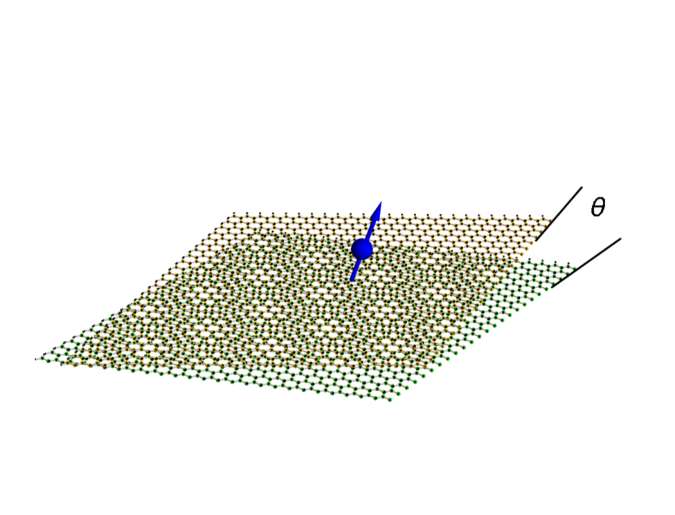
\includegraphics[width=1\linewidth]{figures/chapter2/Kondo_impurity_on_twisted_bilayer_3.pdf}
		\caption{\centering\label{fig:schematic}}
	\end{subfigure}
	\begin{subfigure}[b]{0.47\linewidth}
		\centering
		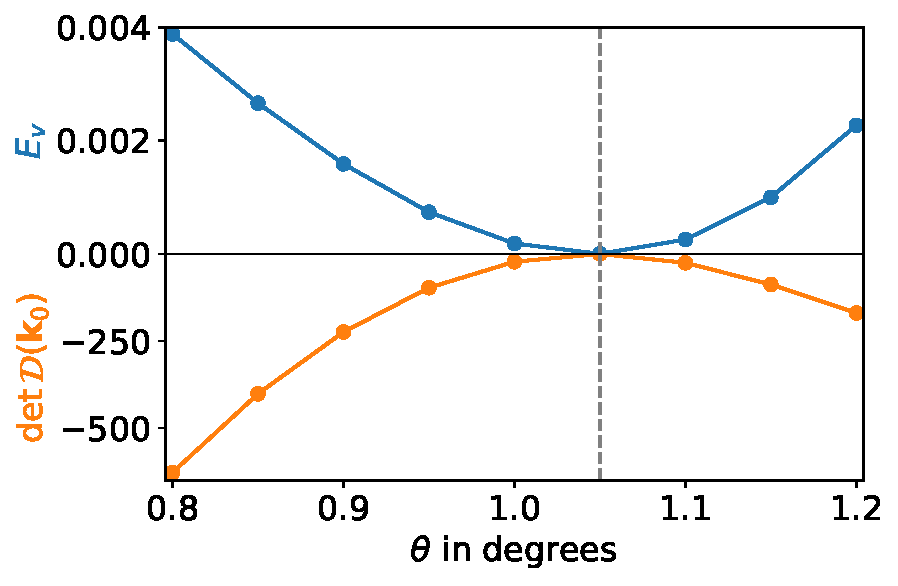
\includegraphics[width=\linewidth]{figures/chapter2/ShowHigherOrder.pdf}
		\caption{\centering{\label{fig:ShowHigherOrder}}}
	\end{subfigure}\\
	\begin{subfigure}[b]{\linewidth}
		\centering
		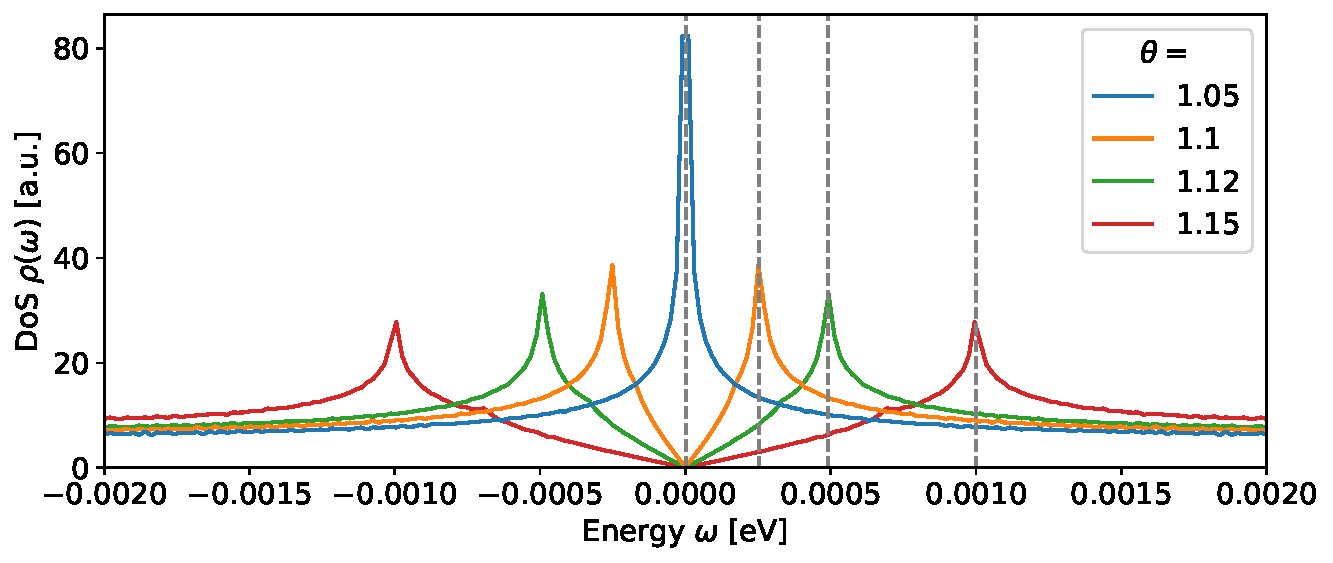
\includegraphics[width=\linewidth]{figures/chapter2/BiggerFontHistogramDOS.pdf}
		\caption{\centering{\label{fig:HistogramDOS}}}
	\end{subfigure}
	\caption{ %\justifying
		  (a) Schematic representation of a magnetic impurity on the surface of the twisted bilayer graphene host material, with inter-layer twist angle $\theta$.   (b) Vanishing vHs saddle point scale $E_v$ (top) and determinant of the saddle point Hessian (bottom) as the magic angle is approached, showing how two vHs's coalesce into a single HO-vHs. 
     (c) Evolution of the clean TBG density of states for different twist angles near the magic angle at $\theta = 1.05^{\circ}$. Vertical dashed lines indicate the energy of the dispersion saddle points $E_v$, which determine the van Hove singularity locations.}
	\label{fig:joinedfig}
\end{figure*}

Specifically, we consider a single, interacting Anderson impurity embedded in the TBG host -- see Fig.~\ref{fig:schematic}. The clean TBG material is modelled using the Bistritzer-MacDonald (BM) model~\cite{Bistritzer2011}, which we discuss in Sec.~\ref{sec:BM-model}. We focus on the role of the vHs's and their evolution with twist angle. The model shows an intricate interplay between different DoS elements: metallic, Dirac pseudogap, vHs log-divergence, and HO-vHs power-law divergence. In Sec.~\ref{sec:Kondo} we review the physics of the Kondo model, emphasizing the different limiting behaviors arising in the metallic, pseudogap, and log-diverging or power-law diverging DoS needed to understand the compound DoS structure in TBG. Finally, in Sec.~\ref{sec:Kondo-BM} we present full numerical renormalization group (NRG) results for an Anderson impurity in TBG in the vicinity of, and at, the magic angle. We focus on thermodynamic quantities such as the impurity entropy as a clear means of identifying the different fixed points and emergent energy scales. We furthermore study the energy-dependence of the local impurity spectral function, which is relevant to STS experiments. We conclude in Sec.~\ref{sec:conclusions}, commenting on the suitability of magnetic impurities as \textit{in-situ} probes for the physics of TBG near the magic angle, and an outlook for experiments. Technical material is given for reference in the Appendices. 

We note that the Kondo model we consider in this work is completely different from recent studies of TBG as a heavy fermion problem~\cite{song2022magic,hu2023kondo,hu2023symmetric,zhou2023kondo}, where the quenched kinetic energy of the flat band lends itself to being treated as an immobile lattice of impurities. In those works, the correlated local moments are a part of the TBG lattice itself, whereas here we consider additional adatom impurities coupled to the TBG host. The effective impurity models and corresponding electronic hybridization functions are rather different in these two cases.


%##########################
%##########################


\section{Van Hove singularities in the Bistritzer-MacDonald model} \label{sec:BM-model}

Before considering a Kondo impurity in TBG, we first analyze the clean host material, focusing on how the vHs's affect the band structure and local DoS. In the first part of this section we briefly recall the details of the Bistritzer-MacDonald (BM) model of TBG and its particle-hole symmetric limit. The original derivations were performed in Refs.~\cite{Bistritzer2011,Suarez2011,Bernevig2019PRL-TBG}; further details are provided in the Appendices. In the second part, we analyze the formation of flat bands from saddle points and discuss the detailed structure of the lowest energy bands.

%################

\subsection{Particle-hole symmetric\\Bistritzer-MacDonald model}

To describe TBG with a small twist angle  $\theta$, it is necessary to take into account both the intralayer hopping parameter $t$ for each of the individual graphene layers, as well as the interlayer tunneling $w$. In the following we take these to be $t\approx 2.87 \,\text{eV}$ and $w\approx 0.11 \,\text{eV}$, as used in Ref.~\cite{Bistritzer2011}. The twist angle between the layers generates a Moir\'{e} pattern with an emergent superlattice structure. For small twist angles $\theta$, the characteristic Moir\'{e} length scale $L_{\theta}$ is given by $L_{\theta}=\sqrt{3} a /[2 \sin (\theta / 2)]$ with $a=1.42\text{\AA}$ being the interatomic distance in monolayer graphene. The corresponding effective low-energy Hamiltonian near the $K$ point of the Moir\'{e} Brillouin zone (MBZ) has the form \cite{Bistritzer2011,Bernevig2019PRL-TBG},
\begin{align}
	\label{eq:H-TBG-full}
	H(\vec{k}) = \left(\begin{array}{cccc}
		h_{\frac{\theta}{2}}^{K}(\vec{k}) & w T_1 & w T_2 & w T_3 \\
		w T_1^{\dagger} & h_{-\frac{\theta}{2}}^{K}(\vec{k}-\mathbf{q}_1) & 0 & 0 \\
		w T_2^{\dagger} & 0 & h_{-\frac{\theta}{2}}^{K}(\vec{k}-\mathbf{q}_2) & 0 \\
		w T_3^{\dagger} & 0 & 0 & h_{-\frac{\theta}{2}}^{K}(\vec{k}-\mathbf{q}_3)
	\end{array}\right).
\end{align}
The wave vector $\vec{k}$ is measured relative to the $K$ point, and the Hamiltonian acts on 8-component wavefunctions $\Psi=\left(\psi_{0, \vec{k}}, \psi_{1, \vec{k}}, \psi_{2, \vec{k}}, \psi_{3, \vec{k}}\right)^T$, where $\psi_{0, \vec{k}}$ is a two-component spinor in the A-B sublattice basis in the top layer, and $\psi_{1(2,3), \vec{k}}$ are spinors in bottom layer at wave vectors $\vec{k}-\vec{q}_{1(2,3)}$.
Here $h_{\phi}^{K}(\vec{k})$ is the effective low-energy Hamiltonian of single layer graphene near the $K$ point, in a coordinate frame rotated by angle $\phi$,
\begin{align}
	h_{\phi}^K(\vec{k})=k v_F \left[\begin{array}{cc}
		0 & e^{i\left(\theta_{\vec{k}}-\phi\right)} \\
		e^{-i\left(\theta_{\vec{k}}-\phi\right)} & 0
	\end{array}\right]\;.
	\label{eq:hKtheta}
\end{align}
Here, the angle $\theta_k$ measures the orientation of the momentum relative to
the $x$-axis, $k=|\vec{k}|$, and the Fermi velocity is $v_F=9.3 \times 10^7 \mathrm{~cm} / \mathrm{s}$. The wave vectors $\vec{q}_{1,2,3}$ connecting $K$-points of the top and bottom layers are,
\begin{subequations}
	\begin{align}
		&\mathbf{q}_1=k_\theta\{0,-1\}, \\
		&\mathbf{q}_2=k_\theta\left\{\frac{\sqrt{3}}{2}, \frac{1}{2}\right\}, \\
		&\mathbf{q}_3=k_\theta\left\{-\frac{\sqrt{3}}{2}, \frac{1}{2}\right\},
	\end{align} 
\end{subequations}
with Moir\'{e} wave number, $k_\theta \equiv |\mathbf{q}_j|=\frac{8 \pi}{3 \sqrt{3} a} \sin \left(\frac{\theta}{2}\right)$.

Finally, the interlayer tunneling matrices $T_{1(2,3)}$ are expressed in terms of Pauli matrices, viz:
\begin{subequations}
	\begin{align}
		&T_1=1+\sigma_x \;,\\
		&T_2=1-\frac{\sigma_x}{2}-\frac{\sqrt{3}\sigma_y}{2} \;,\\
		&T_3=1-\frac{\sigma_x}{2} +\frac{\sqrt{3}\sigma_y}{2}  \;.
	\end{align}
\end{subequations}

The Hamiltonian Eq.~\eqref{eq:H-TBG-full} captures the essential physics of TBG and correctly predicts the first magic angle at $\theta\simeq 1.05^{\circ}$. At the $K$ point of the MBZ one finds that the lowest energy bands have a Dirac cone dispersion with an effective Fermi velocity,
\begin{align}
	v_F^{\star}=\frac{1-3 w^2 /\left(\hbar v_F k_\theta\right)^2}{1+6 w^2 /\left(\hbar v_F k_\theta\right)^2}
\end{align}
which vanishes exactly at the magic angle, where $\hbar v_F k_\theta=\sqrt{3} w$.

In the following, we will use the particle-hole symmetric version of the BM model. This form is obtained from Eq.~\eqref{eq:H-TBG-full} by eliminating subleading (second-order) corrections in the diagonal elements coming from the effect of the twist on the single layer Hamiltonian \cite{Bernevig2019PRL-TBG}. This is simply achieved by setting $\phi=0$ in Eq.~\eqref{eq:hKtheta},
\begin{align}
	\label{eq:H-TBG-symmetric}
	H(\vec{k})=\left(\begin{array}{cccc}
		h_0^{K}(\vec{k}) & w T_1 & w T_2 & w T_3 \\
		w T_1^{\dagger} & h_0^{K}(\vec{k}-\mathbf{q}_1) & 0 & 0 \\
		w T_2^{\dagger} & 0 & h_0^{K}(\vec{k}-\mathbf{q}_2) & 0 \\
		w T_3^{\dagger} & 0 & 0 & h_0^{K}(\vec{k}-\mathbf{q}_3)
	\end{array}\right)\;.
\end{align}

The low-energy TBG DoS $\rho(\omega)$, obtained by diagonalizing this Hamiltonian is shown in Fig.~\ref{fig:HistogramDOS}, for different twist angles in the vicinity of the magic angle at $\theta=1.05^{\circ}$. When precisely at the magic angle, we see a single divergence in the DoS at the Fermi energy. We measure energies relative to the Fermi energy and set $E_F=0$, such that $\rho(\omega)=\rho(-\omega)$, embodying the particle-hole symmetry of Eq.~\eqref{eq:H-TBG-symmetric}. However, moving away from the magic angle, we have a Dirac cone feature, with pseudogap vanishing DoS $\rho(\omega)\sim |\omega|$ below an emergent scale $|\omega|\ll E_v$. We also see two vHs points with diverging DoS at $\omega=\pm E_v$. Below we analyze the low-energy bands and vHs structure of the model, extracting the angle dependence of the vHs scale $E_v$.

%######################

\subsection{Characterization of van Hove singularities in the particle-hole symmetric BM model}

We start our analysis of vHs properties in TBG by recalling the classification recently introduced in Refs.~\cite{Yuan2019,Chamon2020PRR,Yuan2020PRB-classification}, which expands the definition from the usual vHs with logarithmically diverging DoS  \cite{vanHove1953} to include HO-vHs with power-law diverging DoS. For a band dispersion $\epsilon(\vec{k})$, which is a function of the 2D momentum vector $\vec{k}$, we calculate the first derivatives $\nabla_{\vec{k}}\epsilon(\vec{k})$, and the Hessian matrix of second derivatives $\mathcal{D}_{i j}(\vec{k}) \equiv \frac{1}{2} \partial_{k_i} \partial_{k_j} \varepsilon(\vec{k})$. The Hellman-Feynman theorem allows to carry this out with high numerical accuracy (see Appendix~\ref{app:KondoA}). 
A logarithmic vHs arises at a point $\vec{k}_0$ in the dispersion corresponding to a saddle point when:
\begin{align}\label{eq:logvhs}
	\text{log vHs:}\quad \nabla_{\vec{k}}  \varepsilon(\vec{k}_0)=\mathbf{0} \text {~~~and~~} \operatorname{det} \mathcal{D}(\vec{k}_0)<0 \;.
\end{align}
The negative Hessian determinant means that we have both a maximum and a minimum in each of the principal directions of the saddle point. A higher-order saddle point, corresponding to a HO-vHs, is instead characterized by zero determinant of Hessian matrix:
\begin{align}\label{eq:hovhs}
	\text{HO-vHs:}\quad \nabla_{\vec{k}}  \varepsilon(\vec{k}_0)=\mathbf{0} \text {~~~and~~} \operatorname{det} \mathcal{D}(\vec{k}_0)=0 \;.
\end{align}
In addition, higher-order saddle points can be classified according to the leading polynomial terms in an expansion of the dispersion $\epsilon(\vec{k})$ around the saddle point $\vec{k}_0$ \cite{Chamon2020PRR,Yuan2020PRB-classification}. These leading terms in the expansion correspond directly to the numerical exponent of the power-law divergence in the DoS.


\begin{figure*}
	\centering
	\begin{subfigure}[b]{0.475\linewidth}
		\centering
		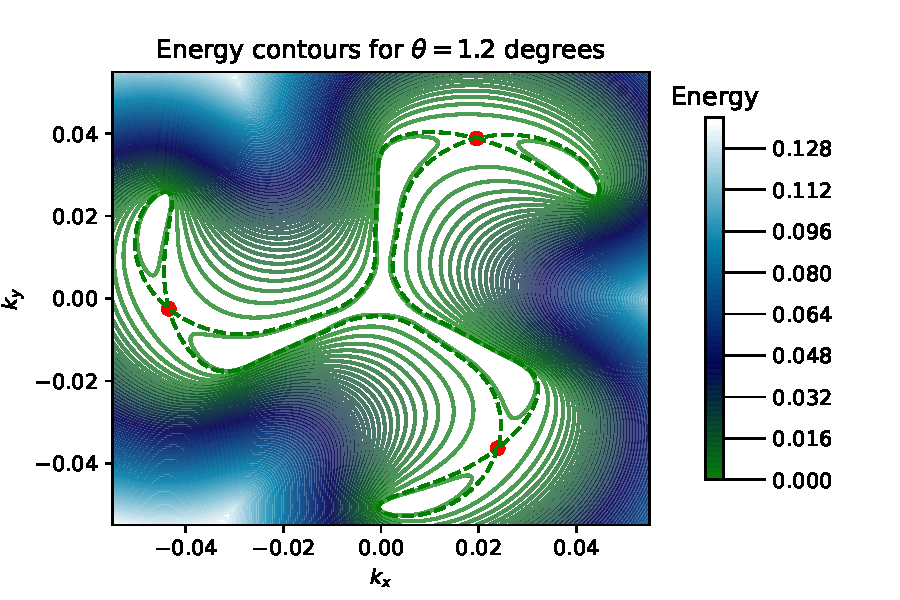
\includegraphics[width=\linewidth]{figures/chapter2/ContoursLog.pdf}
		\caption[ContoursLog]%
		{{  Conventional  vHs}\label{fig:contourslog}}  
	\end{subfigure}
	\hfill
	\begin{subfigure}[b]{0.475\linewidth}   
		\centering 
		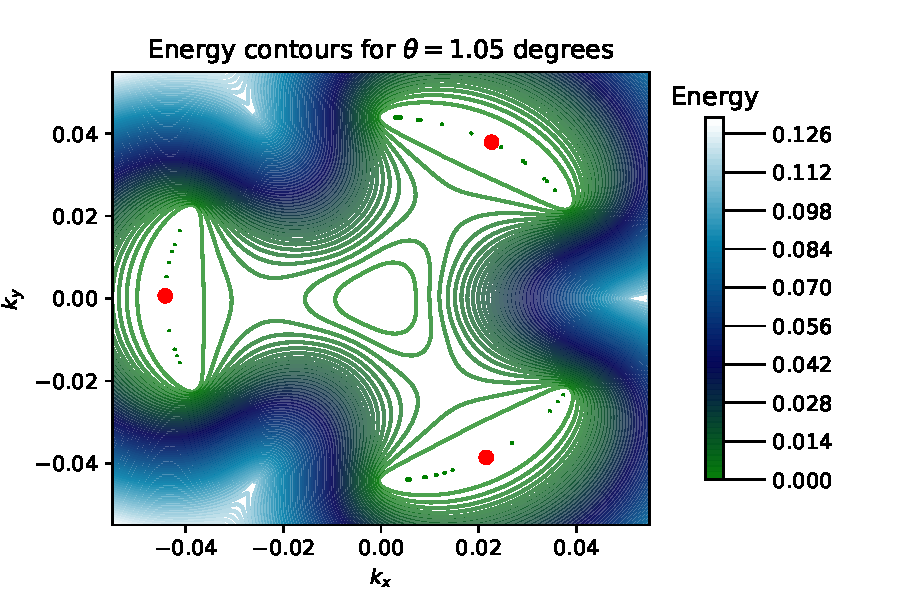
\includegraphics[width=\linewidth]{figures/chapter2/ContoursMagic.pdf}
		\caption[]%
		{{  Higher Order vHs at the magic angle}\label{fig:Magic_Heatmap}}    
	\end{subfigure}
	\caption[ FermiSurfacePlots ]
	{%\justifying
		   Low-energy features of the particle-hole symmetric BM model of pristine TBG, showing energy contours of the dispersion $\varepsilon(\boldsymbol{k})$ as a function of momentum $\boldsymbol{k}$ in the extended MBZ. Red points show the saddle points of the dispersion, corresponding to the van Hove singularities. Dashed lines show the contours at energy $E_v$, on which the van Hove points sit.} 
	\label{fig:Spinners}
\end{figure*}


With the help of this classification, we proceed to investigate the structure of the lowest band in the BM model Hamiltonian given by Eq.~\eqref{eq:H-TBG-symmetric}. Using particle-hole symmetry in conjunction with the transformation $k_x\to -k_x$ allows us to concentrate only on the lowest positive energy band for our analysis. Technical details of our numerical implementation are presented in  Appendix~\ref{app:KondoA}. In Fig.~\ref{fig:ShowHigherOrder} we show the numerically-computed $E_v$ scale (top panel) and the determinant of the saddle-point Hessian $\operatorname{det} \mathcal{D}(\vec{k}_0)$ (bottom panel) as a function of twist angle. Both are seen to vanish at the magic angle, heralding the emergence of the HO-vHs at this point. This behavior is further analyzed below.

In Fig.~\ref{fig:Spinners} we plot the momentum-resolved spectrum of the BM model for twist angles $\theta=1.2^{\circ}$ (panel a) and $\theta=1.05^{\circ}$ (panel b). We compute $\nabla_{\vec{k}} \varepsilon(\vec{k})$ throughout the MBZ and search for the vHs points for which $\nabla_{\vec{k}} \varepsilon(\vec{k})=\vec{0}$. These are indicated in both panels as the red circle points. 

Having located the vHs points in the MBZ for a given twist angle, we can classify them and study their neighborhood in momentum space. Away from the magic angle (e.g.~for $\theta=1.2^{\circ}$ shown in Fig.~\ref{fig:Spinners}a), we indeed find a negative determinant of the Hessian $\operatorname{det} \mathcal{D}(\vec{k}_0)<0$, and the vHs's have a local hyperbolic geometry in momentum space. The dispersion is found to have the leading form,
\begin{equation}
	\epsilon_{\mathbf{p}} = E_v + \alpha p_x^2 - \beta p_y^2 \;, 
	\label{eq:Logdispersion}
\end{equation}
where the coefficients are obtained from the eigenvalues of the Hessian, and the labels $p_x$ and $p_y$ are measured in the principal directions of the saddle point, with $\mathbf{p}=0$ defining the saddle point itself. The corresponding leading correction to the DoS then takes the form,
\begin{equation}
	\rho(\omega) = \frac{1}{4\pi^2}\frac{1}{\sqrt{\alpha\beta}}\ln \abs{\frac{D}{\omega-E_v}} \;,
	\label{eq:logDOS}
\end{equation}
where $D$ is a high-energy cutoff, taken to be the conduction electron bandwidth. In this way, we may extract the vHs scale $E_v$.

As we begin twisting toward the magic angle, the vHs energy scale $E_v$ starts to decrease, and the two logarithmic singularities at $\omega=\pm E_v$ therefore move closer together. Furthermore, the magnitude of the Hessian at the vHs, $|\operatorname{det} \mathcal{D}(\vec{k}_0)|$, also decreases. The two vHs points merge at $\omega=0$ precisely at the magic angle $\theta = 1.05^\circ$ \cite{Li2010}, at which point the Hessian also vanishes, $\operatorname{det} \mathcal{D}(\vec{k}_0)=0$. This transition is shown in Fig.~\ref{fig:ShowHigherOrder}. As the magic angle is approached and the HO-vHs is formed, we see a further flattening of the dispersion in the $p_y$ direction. The fittingly-named higher-order singularity requires a higher-order polynomial to faithfully capture its dispersion. The lowest polynomial which correctly captures all the symmetries is given by,
\begin{equation}
	\epsilon_{\mathbf{p}} = \alpha p_x^2 + \gamma p_x p_y^2 + \kappa p_y^4 \;.
\end{equation}
This comes hand-in-hand with a sharper, power-law divergence in the DoS, 
\begin{equation}\label{eq:HOdos}
	\rho(\omega) = (2\pi)^{-\frac{5}{2}} \Gamma(\tfrac{1}{4})^2 (4\alpha\Tilde{\Gamma}^2)^{-1/4}~ |\omega|^{-\nicefrac{1}{4}} \;, 
\end{equation}
with $\Tilde{\Gamma}^2=\gamma^2 - 4\alpha\kappa $ and $\Gamma(x)$ the usual gamma function. 

The low-energy DoS at different angles can be computed numerically by binning histograms of energies for the lowest band of the BM model, as shown in Fig.\ref{fig:HistogramDOS}. Away from the magic angle, the numerical calculation indicates a linear DoS around the Fermi energy, coming from the Dirac cone in the spectrum. Around $\omega=\pm E_v$ we see the vHs log-divergences. At the magic angle, the HO-vHs around the Fermi energy `eat up' the Dirac cone, and we have instead a large DoS at low energies, diverging as $\rho(\omega)\sim |\omega|^{-1/4}$.


%#####################
%#####################


\section{The Kondo problem}\label{sec:Kondo}

The Kondo effect is a classic paradigm in many-body quantum physics \cite{Hewson}. The corresponding Kondo model features a single quantum spin-$\tfrac{1}{2}$ magnetic impurity coupled by antiferromagnetic exchange to a single channel of non-interacting conduction electrons. Originally, the Kondo model was formulated to describe dilute magnetic impurities such as iron, in bulk metals such as gold \cite{Kondo1970,costi2009kondo}. In these metallic systems, an impurity local moment becomes strongly entangled with its surrounding conduction electrons at low temperatures, and is dynamically screened \cite{bayat2010negativity,mitchell2011real,v2020observation}. This leads to dramatically enhanced spin-flip scattering in the host metal, which can be detected spectroscopically \cite{ternes2008spectroscopic}. 

A more microscopic starting point is provided by the single impurity Anderson model \cite{Hewson}, which describes the impurity as a single quantum orbital with strong electron interactions,
\begin{eqnarray}\label{eq:AM}
	H_{\rm AM} = H_{\rm host} &+ \epsilon_d \sum_{\sigma} d_{\sigma}^{\dagger}d_{\sigma}^{\phantom{\dagger}} + U_d d_{\uparrow}^{\dagger}d_{\uparrow}^{\phantom{\dagger}}d_{\downarrow}^{\dagger}d_{\downarrow}^{\phantom{\dagger}} \nonumber \\ &+ g\sum_{\sigma}\left ( d_{\sigma}^{\dagger} c_{0,\sigma}^{\phantom{\dagger}} + c_{0,\sigma}^{\dagger}d_{\sigma}^{\phantom{\dagger}} \right) \;,
\end{eqnarray}
where $d_{\sigma}^{(\dagger)}$ is an annihilation (creation) operator for an impurity electron with spin $\sigma=\uparrow$/$\downarrow$, and $H_{\rm host}=\sum_{k,\sigma} \epsilon_k c_{k,\sigma}^{\dagger}c_{k,\sigma}^{\phantom{\dagger}}$ describes the clean host. Here $c_{k,\sigma}^{(\dagger)}$ annihilates (creates) a conduction electron of the host material with momentum $k$ and spin $\sigma$. We do not employ band indices in this expression. The impurity couples locally in real-space to the effective host orbital $c_{0,\sigma}=\sum_k \xi_k c_{k,\sigma}$, where $\xi_k$ is the weight of state $k$ at the impurity location (taken to be at the origin).

For small host-impurity hybridization $g$, repulsive Coulomb interaction $U_d>0$, and suitably-chosen impurity potential $-U_d<\epsilon_d<0$, a spin-$\tfrac{1}{2}$ local moment can be trapped on the impurity. Projecting onto this doubly-degenerate spin-$\tfrac{1}{2}$ manifold of impurity states by eliminating virtual excitations to empty or doubly-occupied impurity configurations by means of a Schrieffer-Wolff (SW) transformation \cite{Hewson,schrieffer1966relation} yields the simpler Kondo model,
\begin{eqnarray}\label{eq:KM}
	H_{\rm KM} = H_{\rm host} &+ J \vec{S} \cdot \vec{s}_0 + V\sum_{\sigma}c_{0,\sigma}^{\dagger}c_{0,\sigma}^{\phantom{\dagger}}  \;,
\end{eqnarray}
where $J>0$ is the antiferromagnetic exchange interaction between the impurity spin-$\tfrac{1}{2}$ degree of freedom $\vec{S}$, and the \emph{spin density} of the host conduction electrons at the impurity position $\vec{s}_0=\tfrac{1}{2}\sum_{\alpha,\beta}c^{\dagger}_{0,\alpha} \vec{\sigma}_{\alpha\beta} c^{\phantom{\dagger}}_{0,\beta}$, where $\vec{\sigma}$ is the vector of Pauli matrices. The third term describes potential scattering of the host conduction electrons induced by the impurity (since $c_{0,\sigma}^{\dagger}c_{0,\sigma}^{\phantom{\dagger}}=\sum_{k,k'}\xi_k\xi_{k'}c_{k,\sigma}^{\dagger}c_{k',\sigma}^{\phantom{\dagger}}$). 

The standard Schrieffer-Wolff result \cite{Hewson,schrieffer1966relation}, which becomes exact in the limit $U_d/g^2\to \infty$, yields $J=2g^2[(U_d+\epsilon_d)^{-1} - (\epsilon_d)^{-1}]$ and $V=-g^2[(U_d+\epsilon_d)^{-1} + (\epsilon_d)^{-1}]$. At the particle-hole symmetric point of the model $\epsilon_d=-U_d/2$, we therefore obtain $J=8g^2/U_d$ and $V=0$ (the latter result can be viewed as a many-body quantum destructive interference effect between particle and hole processes). Although the Kondo model Eq.~\eqref{eq:KM} correctly captures the low-energy physics of Eq.~\eqref{eq:AM}, it should be noted that for realistic values of $U_d$, $\epsilon_d$, and $g$ outside of the strict perturbative regime, the values of the effective parameters $J$ and $V$ must be obtained by more sophisticated means that take into account renormalization from the conduction electrons and the specific conduction electron DoS \cite{rigo2020machine}. We also emphasize that $J$ and $V$ are not independent parameters in Eq.~\eqref{eq:KM}, being both derived from the same microscopic parameters of the underlying Anderson model.

The physics of the impurity problem is controlled by the local (free) conduction electron DoS seen by the impurity, $\rho_{\sigma}(\omega)=-\tfrac{1}{\pi}{\rm Im}~\langle\langle c_{0,\sigma}^{\phantom{\dagger}} ; c_{0,\sigma}^{\dagger}\rangle\rangle^{0}$, where $\langle\langle c_{0,\sigma}^{\phantom{\dagger}} ; c_{0,\sigma}^{\dagger}\rangle\rangle$ is the retarded, real-frequency local host Green's function at the impurity position, and the $0$ superscript denotes that it is calculated for the clean host.

In this work we consider a single magnetic impurity (the `dilute limit') embedded in an otherwise clean host TBG system modelled by the BM model. $SU(2)$ spin symmetry is taken to be unbroken. We also assume that the impurity couples equally to all BM bands independently of the impurity position ($\xi_k$ is constant for all momenta and band indices), such that $\rho_{\sigma}(\omega)\equiv \rho(\omega)$ is the TBG DoS, whose low-energy form is described by Eqs.~\eqref{eq:logDOS} or \eqref{eq:HOdos}. \rev{This is certainly a simplification, since details of the impurity-TBG hybridization will naturally affect details of the impurity response. The specific form of the impurity hybridization function will in practice depend on the impurity location within the moir\'e unit cell and how the impurity couples in real-space to the constituent TBG carbon atoms. We leave such \textit{ab initio} studies for future work. However, the rich physics uncovered below will remain qualitatively unaltered provided the impurity hybridization function still features  van Hove divergences flanking a central pseudogap Dirac cone. Since the origin of these features is rooted deeply in the symmetry and topology of the TBG material, we expect the idealized Kondo physics described here to be rather generic. On the other hand, insights from monolayer graphene \cite{mitchell2013kondo} indicate that the physics of vacancies in TBG or substitutional dopants may drastically differ, since the local DoS in these cases is strongly modified.}

In the rest of this section we review the methods that we use to attack the problem as well as the quantities to be analyzed. 

%################+

\subsection{Poor man's scaling approach}\label{subsec:poorman}

The Kondo model as defined by Eq.~\eqref{eq:KM} is a nontrivial strong correlation problem. For metallic host systems, the first insights were provided by Kondo's calculation of the scattering T-matrix \cite{Kondo1970}, which is related to the impurity spectral function. Kondo found a low-temperature divergence in perturbation theory: even when the bare $J$ is small, straight perturbation theory does not give a good description of the low-temperature physics or a proper understanding of the many-body ground state of the system. This divergence was better understood by Anderson's self-coined `poor-man's scaling' approach \cite{anderson1970poor} -- a precursor to the renormalization group (RG). It identified an emergent low-energy scale $T_K$ -- the Kondo temperature -- below which perturbation theory breaks down, and the problem becomes a strong coupling problem. We briefly introduce the method here, since we will employ it in the next section to understand analytically the scaling properties of an impurity in the TBG host. 

Conventionally in the poor man's scaling approach, one uses dimensionless couplings $j=\rho_0 J$ and $v=\rho_0 V$ with $\rho_0=\rho(\omega=0)$ the Fermi level DoS. However, for consideration of Dirac systems where $\rho_0$ may in fact vanish, a different choice is required. Here we simply use the original dimensionful couplings $J$ and $V$. Furthermore, we assume that the host DoS is particle-hole symmetric, meaning $\rho(\omega)=\rho(-\omega)$, a property satisfied by Eq.~\eqref{eq:H-TBG-symmetric}; and is defined within a band of halfwidth $D$, meaning $\rho(\omega)\propto \theta(D-|\omega|)$.

Anderson's scaling procedure goes as follows \cite{anderson1970poor}: (i) integrate out high energy conduction electron states $D-\delta D<|\omega|<D$ close to the band edges in a shell of width $\delta D$; (ii) incorporate the effect of virtual excitations to these eliminated states perturbatively by rescaling the couplings $J$ and $V$ to give an effective Hamiltonian of the same form but defined with a reduced bandwidth $D\to D-\delta D$; (iii) study the flow of the parameters $J$ and $V$ on successive reduction of the bandwidth. Making $\delta D$ infinitessimal, one obtains the following scaling equations,
\begin{eqnarray}\label{eq:poorman}
	\frac{dJ}{d D}&=&-\frac{\rho(D)}{D}J^2 \;, \nonumber \\ 
	\frac{dV}{d D}&=&0\;.
\end{eqnarray}
The first equation determines the flow of the coupling constant $J$ on reducing the bandwidth, whereas the second equation shows that the potential scattering $V$ does not flow. If the bare model is particle-hole symmetric then no potential scattering is generated under the scaling procedure. In the remainder of this paper we will focus on the case $V=0$. The scaling equation for $J$ gives insight into the breakdown of perturbation theory and hence $T_K$, by identifying the point where the rescaled $J$ diverges. We consider various relevant situations in the following. 

%################

\subsection{Numerical Renormalization Group}\label{subsec:nrg}

Wilson's numerical renormalization group \cite{wilson1975renormalization,bulla2008numerical} (NRG) is a non-perturbative technique for solving quantum impurity type problems. It builds upon Anderson's perturbative scaling ideas \cite{anderson1970poor}, but overcomes its limitations by establishing a more general framework in terms of which physical quantities can be calculated numerically-exactly, down to zero temperature. Wilson's original formulation of NRG \cite{wilson1975renormalization}, designed to obtain the thermodynamic properties of a single magnetic impurity in a metal, has since been extended to deal with arbitrary host systems \cite{chen1995kondo,bulla1997anderson,bulla2008numerical}, and to the calculation of dynamical quantities via the full-density-matrix NRG approach \cite{anders2006spin,weichselbaum2007sum}. The former has allowed NRG to be applied to monolayer graphene \cite{vojta2010gate}, and other Dirac systems \cite{mitchell2013TI, mitchell2015kondo}. The latter provides access to highly accurate spectral data, with excellent real-frequency resolution, at any temperature. NRG has also been adapted over the years to extend the range of problems that can be tackled and improve accuracy or efficiency \cite{bulla1998numerical,oliveira1994generalized,bulla2003numerical,pruschke2009energy,mitchell2014generalized,stadler2016interleaved,lee2021computing,rigo2022automatic}, making it the gold-standard method of choice for solving generalized quantum impurity problems.

The basic NRG algorithm \cite{wilson1975renormalization,bulla2008numerical} proceeds as follows. 
(i) The local conduction electron density of states $\rho(\omega)$ of the pristine host material (without the impurity) must first be calculated. \\
(ii) This DoS is then discretized logarithmically by dividing it up into intervals according to the discretization points $\pm D \Lambda^{-n}$, where $D$ is the bare conduction electron bandwidth, $\Lambda>1$ is the NRG discretization parameter, and $n=0,1,2,3,...$. The continuous electronic density in each interval is replaced by a single pole at the average position with the same total weight, yielding $\rho^{\rm disc}(\omega)$.\\
(iii) The conduction electron part of the Hamiltonian $H_{\rm host}$ is then mapped into the form of a `Wilson chain',
\begin{eqnarray}
	H_{\rm host} \to H_{\rm host}^{\rm disc} = \sum_{\sigma}\sum_{n=0}^{\infty} \Big [ &t_n^{\phantom{\dagger}} \left ( f_{n,\sigma}^{\dagger}f_{n+1,\sigma}^{\phantom{\dagger}}+  f_{n+1,\sigma}^{\dagger}f_{n,\sigma}^{\phantom{\dagger}}\right ) \nonumber \\ 
	&+\epsilon_n^{\phantom{\dagger}} f_{n,\sigma}^{\dagger}f_{n,\sigma}^{\phantom{\dagger}} \Big ]\;,\qquad
\end{eqnarray}
where the Wilson chain coefficients $\{t_n\}$ and $\{\epsilon_n\}$ are determined such that the DoS at the end of the chain reproduces exactly the discretized host DoS, that is $-\tfrac{1}{\pi}{\rm Im}~\langle\langle f_{0,\sigma}^{\phantom{\dagger}} ; f_{0,\sigma}^{\dagger}\rangle\rangle = \rho^{\rm disc}(\omega)$. For a system with particle-hole symmetry, $\epsilon_n=0$ for all $n$. Due to the logarithmic discretization, the Wilson chain hopping parameters decay roughly exponentially down the chain, $t_n \sim \Lambda^{-n/2}$, although the precise details are also important since they encode the specific host DoS \cite{bulla2008numerical}.\\ 
(iv) The impurity is coupled to site $n=0$ of the Wilson chain. We define a sequence of Hamiltonians $H_N$ comprising the impurity and the first $N$ Wilson chain sites,
\begin{equation}\label{eq:Hn}
	\begin{split}
		H_N=&H_{\rm imp} + H_{\rm hyb} + \sum_{\sigma}\Bigg [ \sum_{n=0}^{N} 
		\epsilon_n^{\phantom{\dagger}} f_{n,\sigma}^{\dagger}f_{n,\sigma}^{\phantom{\dagger}}\\
		&+ \sum_{n=0}^{N-1}  t_n^{\phantom{\dagger}} \left ( f_{n,\sigma}^{\dagger}f_{n+1,\sigma}^{\phantom{\dagger}}+  f_{n+1,\sigma}^{\dagger}f_{n,\sigma}^{\phantom{\dagger}}\right ) \Bigg ] \;,
	\end{split}
\end{equation}
where for the Anderson model $H_{\rm imp} =\epsilon_d \sum_{\sigma} d_{\sigma}^{\dagger}d_{\sigma}^{\phantom{\dagger}} + U_d d_{\uparrow}^{\dagger}d_{\uparrow}^{\phantom{\dagger}}d_{\downarrow}^{\dagger}d_{\downarrow}^{\phantom{\dagger}}$ and $ H_{\rm hyb}= g\sum_{\sigma} ( d_{\sigma}^{\dagger} f_{0,\sigma}^{\phantom{\dagger}} + f_{0,\sigma}^{\dagger}d_{\sigma}^{\phantom{\dagger}})$ while for the Kondo model $H_{\rm imp} + H_{\rm hyb}=J \vec{S} \cdot \vec{s}_0 + V\sum_{\sigma}f_{0,\sigma}^{\dagger}f_{0,\sigma}^{\phantom{\dagger}}$ with $\vec{s}_0=\tfrac{1}{2}\sum_{\alpha,\beta}f^{\dagger}_{0,\alpha} \vec{\sigma}_{\alpha\beta} f^{\phantom{\dagger}}_{0,\beta}$. From Eq.~\eqref{eq:Hn} we obtain the recursion relation,
\begin{equation}\label{eq:recursion}
	\begin{split}
		H_{N}=&H_{N-1}+\sum_{\sigma}\Big [\epsilon_N^{\phantom{\dagger}} f_{N,\sigma}^{\dagger}f_{N,\sigma}^{\phantom{\dagger}}\\&+ t_N^{\phantom{\dagger}} \left ( f_{N-1,\sigma}^{\dagger}f_{N,\sigma}^{\phantom{\dagger}}+f_{N,\sigma}^{\dagger}f_{N-1,\sigma}^{\phantom{\dagger}}\right ) \Big ] \;,
	\end{split}
\end{equation}
such that the full (discretized) model is obtained as $H^{\rm disc}=\lim_{N\to \infty} H_N$ \cite{note_nrg}. \\
(v) Starting from the impurity, we build up the chain by successively adding Wilson chain sites using the recursion, Eq.~\eqref{eq:recursion}. At each step $N$, the intermediate Hamiltonian $H_N$ is diagonalized, and only the lowest $N_s$ states are retained to construct the Hamiltonian $H_{N+1}$ at the next step (the higher energy states are discarded). In such a way, we focus on progressively lower energy scales with each iteration. Furthermore, the iterative diagonalization and truncation procedure can be viewed as an RG transformation \cite{wilson1975renormalization}, $H_{N+1}=\mathcal{R}[H_N]$.\\
(vi) The partition function $Z_N$ can be calculated from the diagonalized Hamiltonian $H_N$ at each step $N$. Wilson used RG arguments to show \cite{wilson1975renormalization} that thermodynamic properties obtained from $Z_N$ at an effective temperature $T_N \sim \Lambda^{-N/2}$ accurately approximate those of the original undiscretized model at the same temperature. The sequence of $H_N$ can therefore be viewed as coarse-grained versions of the full model, which faithfully capture the physics at progressively lower and lower temperatures.\\
(vii) The discarded states at each step form a complete set (the Anders-Schiller basis \cite{anders2006spin}), from which the NRG full density matrix can be constructed. This provides a rigorous way of calculating real-frequency dynamical quantities via the Lehmann representation \cite{weichselbaum2007sum}.

In this work, we take the DoS $\rho(\omega)$ of the TBG system for a given twist angle $\theta$ (as calculated from the BM model in Sec.~\ref{sec:BM-model}), discretize it logarithmically, and map to Wilson chains. The DoS used and the resulting Wilson chains are shown in Appendix~\ref{app:KondoB}. NRG is then used to solve the Anderson and Kondo models describing an impurity embedded in the TBG host. Thermodynamic and dynamical quantities are calculated and discussed in Sec.~\ref{sec:Kondo-BM}. Throughout, we use an NRG discretization parameter $\Lambda=2$ and retain $N_s=4000$ states at each step of the calculation.

%##################

\subsection{Observables}
\label{sec:obs} 

The physics of an impurity in the TBG host can be characterized by a number of observables, both thermodynamic and dynamical. 
Here we consider the impurity contribution to the total thermal entropy $S_{\rm imp}(T)$ as a function of the temperature $T$, and the low-$T$ impurity spectral function $A(\omega)$ as a function of energy $\omega$. 

The impurity entropy readily allows us to extract the Kondo scale $T_K$ from NRG data, to track accurately the RG flow, and to identify RG fixed points. It is defined as $S_{\rm{imp}}(T) = S_{\rm{tot}}(T) - S_0(T)$, where $S_{\rm{tot}}$ is the entropy of the entire system, while $S_0$ is the entropy of the free TBG host without impurities. The residual  impurity entropy $S_{\rm imp}(T=0)$, is a finite universal number of order unity which characterizes the stable RG fixed point and hence the ground state of the system; for example $S_{\rm imp}(0)=\ln 2$ for a free, unscreened impurity spin $S=\tfrac{1}{2}$ local moment.

The impurity spectral function gives dynamical information and is accessible experimentally via scanning tunneling spectroscopy (STS), which probes the energy-resolved impurity density of states \cite{ternes2008spectroscopic}. For an Anderson impurity it is related to the impurity Green's function, $A(\omega)=-\tfrac{1}{\pi}{\rm Im}~G_{dd}(\omega)$ where $G_{dd}(\omega)=\langle\langle d_{\sigma}^{\phantom{\dagger}} ; d_{\sigma}^{\dagger}\rangle\rangle$. 

Electronic scattering in the TBG system induced by the impurity is characterized by the t-matrix, which in turn is controlled by the impurity Green's function. In momentum space, the t-matrix equation reads,
\begin{equation}
	G_{kk'}(\omega) = \delta_{kk'}G_{kk}^0(\omega) + G_{kk}^0(\omega)T_{kk'}(\omega) G_{k'k'}^0(\omega) \;,
\end{equation}
where $G_{kk'}^{(0)}(\omega)=\langle\langle c_{k,\sigma}^{\phantom{\dagger}} ; c_{k',\sigma}^{\dagger}\rangle\rangle^{(0)}$ is the electron Green's function for the full (free) TBG system with (without) the impurity, and $T_{kk'}(\omega)=g^2\xi_k\xi_{k'}G_{dd}(\omega)$ is the t-matrix itself. Transforming to real space, the t-matrix equation becomes,
\begin{equation}
	G_{\vec{r}_i\vec{r}_j}(\omega) = G_{\vec{r}_i\vec{r}_j}^0(\omega)  + G^0_{\vec{r}_i\vec{r}_0}(\omega) T(\omega) G^0_{\vec{r}_0\vec{r}_j}(\omega) \;,
\end{equation}
where $G_{\vec{r}_i\vec{r}_j}^{(0)}(\omega)$ are the full (free) electronic propagators between real-space sites $\vec{r}_i$ and $\vec{r}_j$ of the TBG system, and the local t-matrix is $T(\omega)=g^2 G_{dd}(\omega)$. The impurity is taken to be located at site $\vec{r}_0$.

A related experimental quantity obtained by Fourier transform STS \cite{hoffman2002imaging} (FT-STS) is the quasiparticle interference (QPI) pattern, defined as,
\begin{equation}
	\Delta \rho(\vec{q},\omega) = \sum_i e^{-i\vec{q}\cdot \vec{r}_i}\Delta \rho(\vec{r}_i,\omega) \;,
\end{equation}
where $\Delta \rho(\vec{r}_i,\omega)=-\tfrac{1}{\pi}{\rm Im}~[G_{\vec{r}_i\vec{r}_i}(\omega)-G_{\vec{r}_i\vec{r}_i}^0(\omega)]$ is the difference in electronic density at site $\vec{r}_i$ due to the impurity. As such, the QPI pattern $\Delta \rho(\vec{q},\omega)$ can be obtained entirely from the free TBG propagators and the impurity Green's function, via the t-matrix equation.

In the following, we study the zero temperature, $T=0$, impurity spectral function $A(\omega)$ using NRG; the t-matrix and QPI can be obtained from this as described above.


%%%%%%%%%%%%%%%%%%%%%%%%%%%%%%%%%%%%%%%%%%%%%%%%%%%%%


\subsection{Limiting cases of the Kondo problem}\label{sec:KondoDOS}

The physics of the Kondo model strongly depends on the host DoS. For the problem of a magnetic impurity in a TBG host, as modelled using the BM model, there are a number of relevant limits. We assume that the impurity couples to all the orbitals in the same way meaning the local TBG DoS $\rho(\omega)$ is the only relevant quantity characterizing the host. Furthermore, we consider here the particle-hole symmetric case $V=0$ for simplicity.

The main insights of the ensuing discussion are summarized in Table~\ref{tab:ScalingTk}.

\begin{small}
\begin{table*}
	\centering
	\begin{tabular}{lccc} \hline\hline
		& Density of States, $\rho(\omega)$   &  ~~Kondo Temperature, $T_K$~~ &  $S_{\rm{imp}}(T=0)$~~ \\ \hline 
		Metal   & $\rho_0$  & $  D e^{-{\nicefrac{1}{\rho_0 J}}}$ & $0$ \\ 
		vHS  & $ \rho_0 \left[1+a\ln \left(D/|\omega| \right) \right]$  & $ D e^{\frac{1}{a} - \frac{1}{a}\sqrt{1 + \frac{2a}{\rho_0J}}}$ & $0 $ \\
		HOvHS & $ \rho_0\abs{\omega}^{-\alpha}$  & $D\left(1+\frac{\alpha D^\alpha}{\rho_0 J}\right)^{-\nicefrac{1}{\alpha}} $ & $-2\alpha \ln 2$\\ 
		Dirac & $\rho_0 |\omega|$  & $T_K=0$ & $\ln 2$\\ \hline\hline
	\end{tabular}
	\caption{Summary of properties for the Kondo model with the different host DoS encountered in this work.}
	\label{tab:ScalingTk}
\end{table*}
\end{small}
%##########

\subsubsection{The metallic limit}\label{subsec:SKondo}

The case of a magnetic impurity embedded in a metallic host is the most commonly encountered and well-studied situation, with extensive literature to its name (see Ref.~\cite{Hewson} for an introduction). The most important feature of the problem is that upon reducing the temperature, the system becomes increasingly strongly correlated. This is captured by the poor-man's scaling equation, Eq.~\eqref{eq:poorman}. In a metal, it is a reasonable assumption that the DoS is roughly constant within the relevant energy window, $\rho(\omega)\approx \rho_0$. Integrating  Eq.~\eqref{eq:poorman} then straightforwardly yields, 
\begin{eqnarray}
	J(\Lambda)=\frac{J_0}{1+\rho_0 J_0 \ln \left( \frac{\Lambda}{D}\right)}\;,
\end{eqnarray}
where $\Lambda$ is the energy scale of interest whereas $D$ is the starting high-energy cutoff (physically $D$ is the conduction electron bandwidth). $J_0$ is the starting value of the coupling constant at the scale $D$ (with $J_0\equiv J$ in Eq.~\eqref{eq:KM}) whereas $J(\Lambda)$ is the running coupling strength at energy scale $\Lambda$. Perturbation theory breaks down, once the running coupling $J(\Lambda=T_K)\to \infty$. This happens at the root of the denominator and the corresponding running energy scale reads
\begin{eqnarray}
	T_K=D e^{-1/(\rho_0 J_0)}\;.
\end{eqnarray}
This energy scale has a number of interpretations. One implication is that for temperatures $T \gg T_K$, the physics can be captured using a perturbative expansion around $J=0$, meaning the limit of a free impurity henceforth referred to as the local moment (LM) regime. Consequently, the impurity entropy, up to small correction, is that of a free spin, meaning $S_{\rm{imp}}^{\rm LM}=\log 2$. 

Conversely, for $T \sim  T_K$, perturbation theory breaks down. Nozi\`eres showed~\cite{nozieres1980kondo} that at zero temperature, the ground state is a complicated many-body spin-singlet state and the system is a local Fermi liquid. The low-temperature limit $T\ll T_K$ is referred to as the strong coupling (SC) regime.  The corresponding impurity entropy is that of a unique state with $S_{\rm{imp}}^{\rm SC}=0$. The strong coupling physics in this regime shows up in the local spectral function $A(\omega)$ as a strong quasiparticle resonance around the Fermi energy, with a spectral pinning condition satisfying the Friedel sum rule \cite{Hewson}. The RG flow between the two fixed points is relatively simple, with $J(\Lambda)$ increasing from LM to SC as the energy scale $\Lambda$ is decreased. This is illustrated in the upper panel of Fig.~\ref{fig:RGFlow}. The Kondo scale $T_K$ is the scaling invariant along this RG flow. Note that in the metallic case, the potential scattering $V$ is strictly marginal and consequently plays no role. 

%##########

\subsubsection{Close to a van Hove singularity}

This case is a twist on the usual metallic Kondo problem, with very similar physics. The poor man's scaling analysis points to an RG flow from weak to strong coupling, with the running coupling $J(\Lambda)$ again increasing from LM to SC as the energy scale $\Lambda$ is decreased (Fig.~\ref{fig:RGFlow}, upper panel). The main difference from the standard metallic case is an enhanced Kondo temperature~\cite{Gogolin1993,Zhuravlev2011,zhuravlev2018one} due to the enhanced DoS, which diverges logarithmically at low energies for standard vHs points. 
Taking the low-energy form of the DoS to be $\rho(\omega)= \rho_0 \left(1+a\ln \left(D/|\omega| \right) \right)$, we can integrate Eq.~\eqref{eq:poorman} and, as before, extract the Kondo scale from the divergence in $J(\Lambda)$. In this case we obtain,
\begin{eqnarray}
	T_K=D e^{\frac{1}{a} - \frac{1}{a}\sqrt{1 + \frac{2a}{\rho_0J_0}}}\;. 
	\label{eq:TKLog}
\end{eqnarray}
Note that for $a \to 0$ the DoS becomes metallic and we recover the metallic limit result for $T_K$.

This expression has two limiting cases and the relevant parameter is now $a/(\rho_0 J_0)$: (i) For $a/(\rho_0 J_0) \ll 1$, the logarithmic enhancement of the DoS plays no role and one recovers the metallic limit result, $T_K=D e^{-1/(\rho_0 J_0)}$ since the system starts out already close to the SC fixed point; (ii) In the opposite limit, $a/(\rho_0 J_0) \gg 1$, we find $T_K=D e^{- \sqrt{\frac{2}{a \rho_0J_0}}}$, which is strongly boosted relative to the metallic case.
The Kondo temperature $T_K$ is therefore enhanced in the vicinity of a vHs. As expected, the impurity entropy is quenched at low temperatures, $S_{\rm{imp}}(T\to 0)=0$, embodying Kondo singlet formation. In terms of the impurity spectral function $A(\omega)$, the quasiparticle Kondo resonance around the fermi energy is in fact suppressed logarithmically by the logarithmically diverging DoS of the free host \cite{derry2015quasiparticle}. However,  the fact that $A(\omega=0)=0$ should not in this case be interpreted as a flow towards weak coupling since the relevant quantity is rather $\rho(\omega)\times A(\omega)$, which remains finite as $|\omega|\to 0$ and satisfies a generalized Friedel sum rule \cite{logan2014common} for strong coupling physics.

%##########

\subsubsection{Close to a Higher Order van Hove singularity}

As discussed in Sec.~\ref{sec:BM-model}, a HO-vHs is characterized by a power-law divergence in the DoS. In the following discussion, we neglect the metallic background on top of which the power-law divergence sits, and take the DoS to be of the form $\rho(\omega)=\rho_0 |\omega|^{-\alpha}$ with $0<\alpha<1$. This problem falls into the class of power-law Kondo problems~\cite{Mitchell2013}. Intuitively, one expects the Kondo temperature to be further enhanced through the more strongly divergent DoS. Integrating Eq.~\eqref{eq:poorman}  with this DoS yields,
\begin{eqnarray}\label{eq:tkHO}
	T_K = \frac{D}{\left(1+\frac{\alpha D^\alpha}{\rho_0 J_0}\right)^{\nicefrac{1}{\alpha}}}\;.
\end{eqnarray}
This problem also has two limits, one characterized by the local moment physics of a free impurity (LM) the other limit by a particle-hole symmetric strong coupling fixed point that we henceforth call $\rm{SSC}_{\rm{HO}}$. This RG fixed point has properties that are slightly different from the metallic strong coupling fixed point SC. It is characterized by a $T \to 0$  impurity entropy of $S_{\rm{imp}}=-2\alpha \ln 2$, which is negative. We emphasize that although the total thermodynamic entropy is of course never negative, the \emph{impurity contribution} to the total system entropy as defined in Sec.~\ref{sec:obs} can be negative, if the presence of the impurity causes dramatic changes to the host (local) electronic structure, relative to the clean host. This is precisely the case for the power-law Kondo model \cite{Mitchell2013}. 
As for the impurity spectral function, the quasiparticle Kondo resonance is suppressed by the divergent free host DoS, and we find $A(\omega) \sim |\omega|^{\alpha}$ at low energies. But again, the signature of Kondo singlet formation and strong coupling physics is that $\rho(\omega)\times A(\omega)$ remains finite as $|\omega|\to 0$, which is indeed the case for $\rm{SSC}_{\rm{HO}}$.

The RG flow in the particle-hole symmetric case considered here is again one-dimensional, running from LM to $\rm{SSC}_{\rm{HO}}$ as the energy scale or temperature is reduced (see middle panel of Fig.~\ref{fig:RGFlow}). We note that strong particle-hole asymmetry can play a role in the power-law Kondo model, unlike the pure metallic case, and leads to the intricate phase diagram discussed in Ref.~\cite{Mitchell2013}.

\begin{figure}[h]
        \centering
	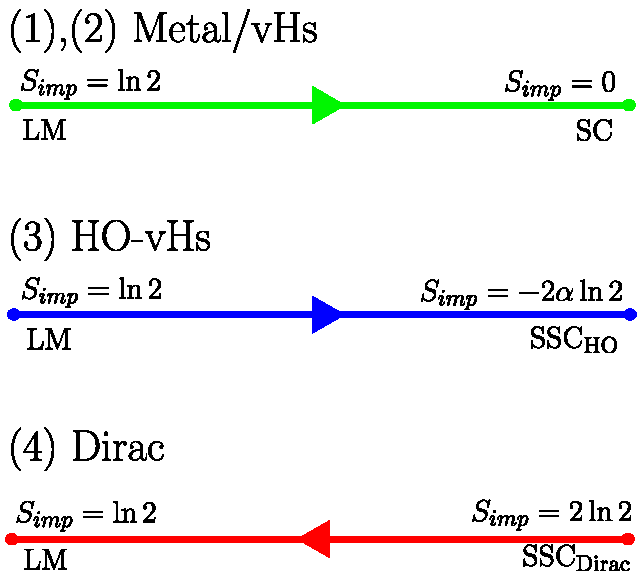
\includegraphics[width=0.5\linewidth]{figures/chapter2/FigureFixPointv4.pdf}
	\caption{
		%\justifying
		   One-dimensional RG diagram showing the flow into different stable fixed points as the temperature is lowered, for different host density of states profiles.}
	\label{fig:RGFlow}
\end{figure}
%##########

\subsubsection{The limit of a two-dimensional Dirac cone}

The linear vanishing DoS associated with a Dirac cone in two dimensional systems gives rise to a subtle impurity problem which falls into the class of so-called pseudogap Kondo models. This is by far the most complicated situation; it has been discussed at length in Refs.~\cite{Ingersent1998,Fritz2004a,Fritz2004b,Fritz2013,logan2014common}. In the following, we focus on the particle-hole symmetric case, with a linear pseudogap $\rho(\omega)=\rho_0|\omega|$ that is characteristic of 2d Dirac materials. Naively, one might expect a reduced Kondo temperature due to the reduced DoS of a Dirac cone compared with that of a metal. In fact, the Kondo effect is suppressed entirely in this case and $T_K$ vanishes, regardless of the strength of the bare coupling $J_0$. The LM fixed point is stable and the impurity local moment remains unscreened.

For large bare $J_0$ the system starts off close to the particle-hole symmetric strong coupling fixed point of the linear pseudogap Kondo model, dubbed $\rm{SSC}_{\rm{Dirac}}$. In this regime, the impurity entropy is $S_{\rm{imp}}=2 \ln 2$. However, this fixed point is unstable and RG flow on reducing the temperature tends towards the LM fixed point with entropy $S_{\rm{imp}}=\ln 2$. Unlike the other cases considered, here the renormalized running coupling $J(\Lambda)$ \emph{decreases} on reducing temperature, so that the impurity always becomes asymptotically free as $T\to 0$. This is illustrated in the lower panel of  Fig.~\ref{fig:RGFlow}. The Kondo effect can only be revived by doping so that the Dirac point is not longer at the fermi energy (in which case the low-energy DoS is finite and we recover the metallic scenario); or if very strong potential scattering is introduced.
For the linear pseudogap case $\rho(\omega)\sim |\omega|$ the impurity spectral function also goes as $A(\omega)\sim |\omega|$. Note that in this case $\rho(\omega)\times A(\omega) \to 0$ as $|\omega|\to 0$, indicating a free impurity at low energies.


%###############
%###############


\section{Results and discussion}\label{sec:Kondo-BM}
We now turn to our full NRG results for a magnetic impurity embedded in the TBG host. The impurity is taken to be of Anderson type (Eq.~\ref{eq:AM}), and the BM model is used for the host (Eq.~\ref{eq:H-TBG-symmetric}). The observables of primary interest are the temperature-dependence of the entropy $S_{\rm imp}(T)$, and the energy-resolved impurity spectral function $A(\omega)$ at $T=0$, for TBG systems with different twist angles  -- see Fig.~\ref{fig:angles}. The most dramatic changes are observed in the vicinity of the magic angle at $\theta=1.05^{\circ}$, and this is where we focus our discussion. The physical quantities we calculate reveal a complex RG flow in the system, illustrated in Fig.~\ref{fig:flow}. The physics precisely at the magic angle is also investigated in detail, and the dependence of the Kondo temperature on microscopic parameters is extracted -- see Fig.~\ref{fig:kondomagic}.
\begin{figure}[H]
        \centering
	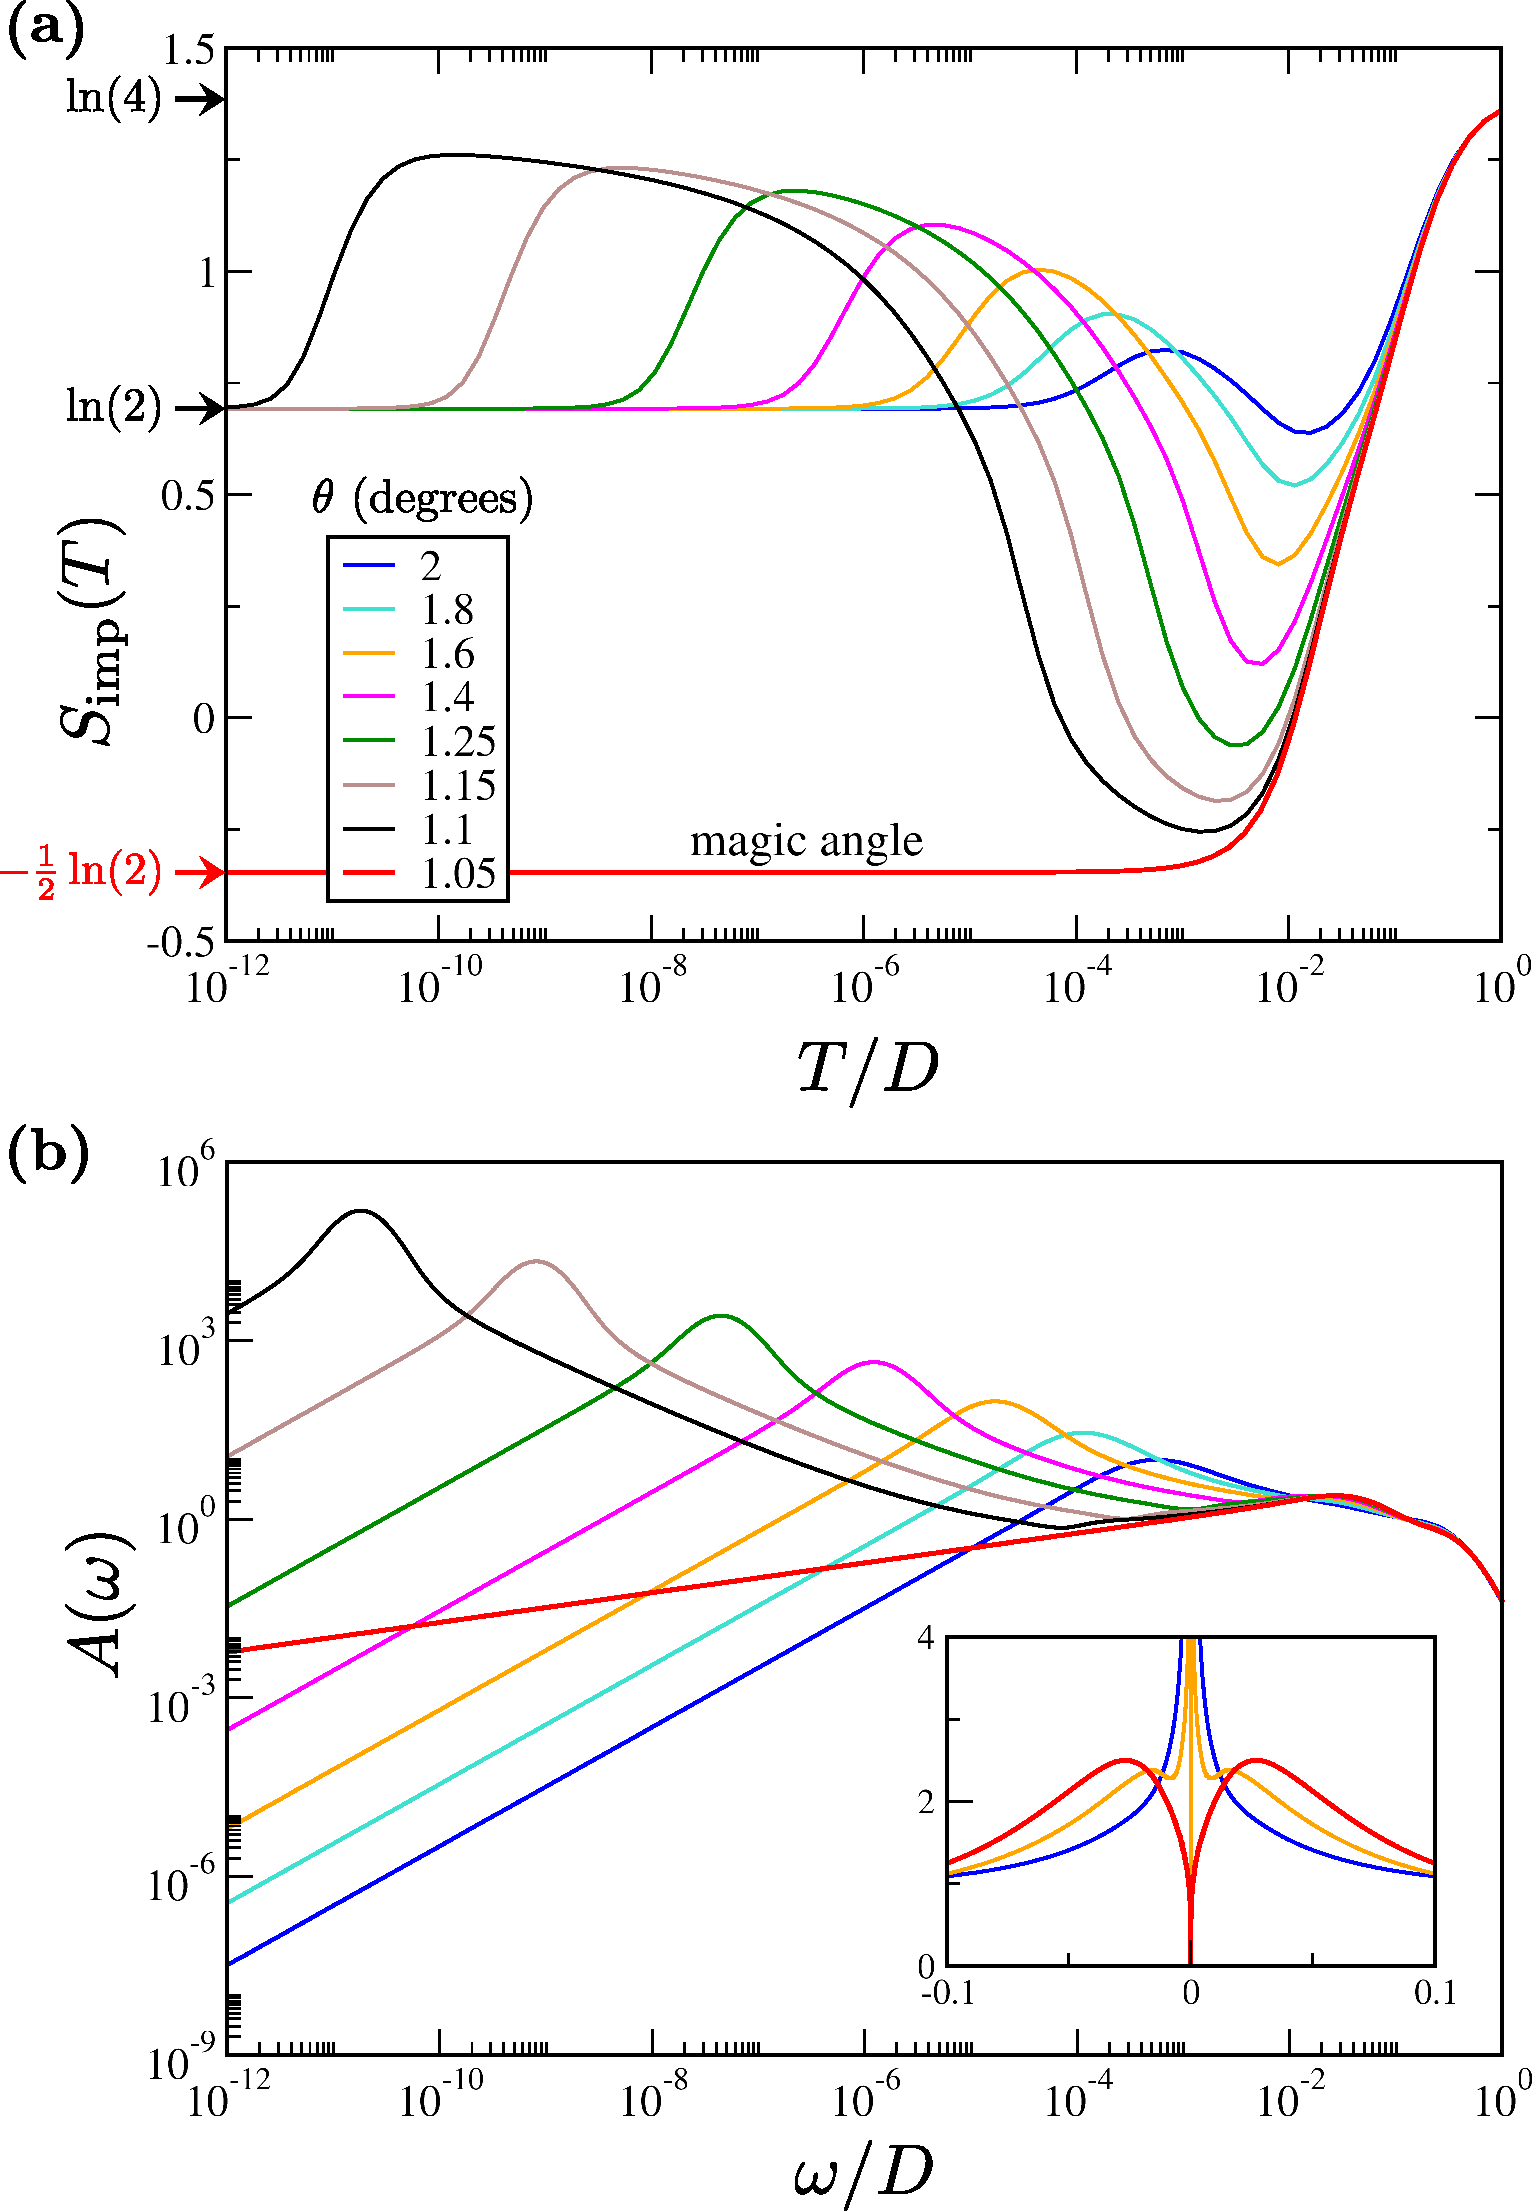
\includegraphics[width=0.6\linewidth]{figures/chapter2/S_A_vs_th.pdf}
	\caption{
		%\justifying
		   NRG results for an Anderson impurity in the TBG host material described by the BM model, at various twist angles $\theta$ approaching the magic angle at $\theta=1.05^{\circ}$. 
		(a) Impurity entropy $S_{\rm imp}(T)$ vs temperature $T$; and (b) Impurity spectral function $A(\omega)$ vs energy $\omega$ at $T=0$. Inset shows low-energy spectral details on a linear scale for representative cases approaching the magic angle. All plots shown for $U_d=0.4D$, $\epsilon_d=-U_d/2$ and $g=0.2D$, with $D$ the TBG bandwidth. }
	\label{fig:angles}
\end{figure}

Consider first the entropy flows presented in Fig.~\ref{fig:angles}(a). At the highest temperatures $T\sim D$, the impurity has four thermally populated configurations (empty, doubly-occupied, and up/down spin states) and the entropy for all systems is therefore $\ln(4)$ in this limit. On the scale $T \sim U$ the empty and doubly-occupied impurity configurations become thermally inaccessible and only the local moment states of the impurity survive. Note that this high-$T$ charge-freezing crossover is absent in the Kondo model, which features only the two impurity spin states from the outset. Far away from the magic angle, where the low-energy TBG DoS is dominated by the linear pseudogap of the Dirac cone, the Kondo effect is inoperative and the impurity spin degrees of freedom remain unscreened down to $T=0$. The impurity entropy therefore saturates at the LM value of $\ln(2)$. This is the basic picture for the blue line in Fig.~\ref{fig:angles}(a) obtained for twist angle $\theta=2^{\circ}$. In the opposite limit, when the system is tuned to the magic angle $\theta=1.05^{\circ}$  the impurity physics is dominated by the power-law divergence in the low-energy DoS of TBG. The physics in this case is effectively that of the power-law Kondo model discussed in the previous section. Since $\rho(\omega)\sim |\omega|^{-1/4}$, the entropy saturates to $-\tfrac{1}{2}\ln(2)$ for $T\ll T_K$, where the Kondo scale $T_K$ itself is strongly enhanced. This is precisely what we observe for the red line in Fig.~\ref{fig:angles}(a).

However, the situation is much more complex for twist angles close to (but not at) the magic angle. To understand the full RG flow in this intermediate regime, consider Fig.~\ref{fig:flow}, together with the fixed point discussion in Sec.~\ref{sec:KondoDOS} and the RG flow diagrams in Fig.~\ref{fig:RGFlow}. Note that the same color-coding is used in Figs.~\ref{fig:RGFlow} and \ref{fig:flow}.

Near the magic angle, the TBG host DoS has a compound structure featuring multiple elements, each of which corresponding to a different limiting Kondo problem. At high energies, the system shows behavior that is characteristic of the HO-vHs, denoted in blue in Fig.~\ref{fig:flow}. This behavior crosses over to that of a standard logarithmic vHs on the scale of $E_v$, denoted in green. Far below this scale, the linear vanishing pseudogap DoS of the Dirac cone emerges, denoted in red. Depending on the energy window, the RG flow will therefore be controlled by the different regimes depicted in  Fig.~\ref{fig:RGFlow}.

\begin{figure}[t]
        \centering
	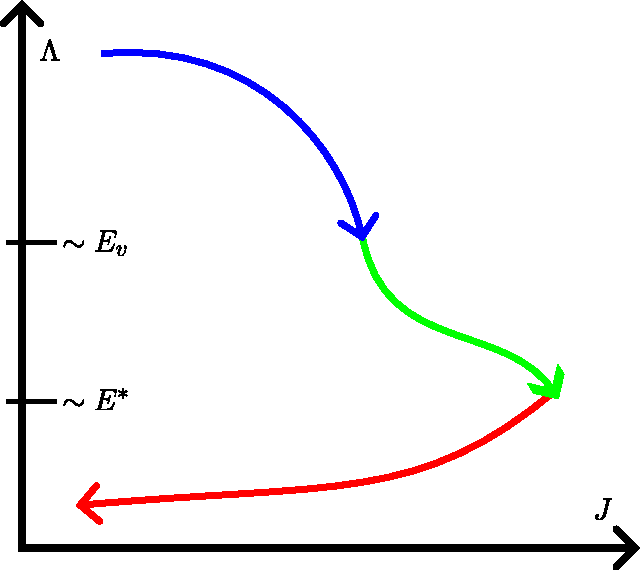
\includegraphics[width=0.4\linewidth]{figures/chapter2/RGFlowColors.pdf}
	\caption{
		%\justifying
		  Near the magic angle, the TBG host DoS has a compound structure. At high energies $\Lambda$, the power-law diverging DoS associated with the HO-vHs generates a rapid RG flow towards strong coupling -- blue arrow. On the scale of $E_v$ the DoS crosses over to logarithmic vHs -- green arrow. Below $E_v$ the Dirac cone pseudogap dominates the DoS and $J(\Lambda)$ begins to decrease again as the system flows back towards the free local moment regime on an emergent scale $E^*$. The color-coding is the same as that in Fig.~\ref{fig:RGFlow}.}
	\label{fig:flow}
\end{figure}



This RG flow is reflected in the temperature dependence of the entropy. After the charge degrees of freedom are frozen out on the high-temperature scale of $T\sim U$ and the impurity entropy reaches $\sim \ln(2)$ characteristic of the LM regime, the system then rapidly flows towards $\rm{SSC}_{\rm{HO}}$ on further reducing the temperature. On this trajectory, the effective coupling strength $J(\Lambda)$ grows as the energy scale $\Lambda$ decreases, and the entropy approaches $S_{\rm{imp}}=-\tfrac{1}{2} \ln 2$. 
However, at the scale $E_v$ the physics of the logarithmic vHs takes over and the system starts  to flow towards the regular SC fixed point with $S_{\rm{imp}}=0$. The running coupling $J(\Lambda)$ continues to increases. 
But on the `other side' of the vHs in energy space, as the temperature is further decreased, the effect of the low-energy pseudogap DoS begins to dominate. Interestingly though, at this point in the RG flow the system already has a very strong coupling strength $J(\Lambda)$, which puts the system close to the unstable $\rm{SSC}_{\rm{Dirac}}$ fixed point. The entropy therefore `overshoots' up to $\ln(4)$ characteristic of this fixed point. The ultimate RG flow on the lowest energy scales is therefore between $\rm{SSC}_{\rm{Dirac}}$ and the stable LM fixed point of the pseudogap Kondo problem, with a residual $T=0$ entropy of $\ln(2)$. The ground state is an unscreened local moment with $\ln(2)$ entropy in all cases except when precisely at the magic angle (where $E_v = 0$ such that this final part of the flow towards LM is omitted). Our NRG results for the entropy show that the final low-temperature flow between $\rm{SSC}_{\rm{Dirac}}$ and LM is controlled by an emergent energy scale $E^* \sim |E_v|^3$.
As we get closer to the magic angle, the $E_v$ scale reduces and the lines fold progressively onto that of the red line for the magic angle itself. The $E^*$ scale rapidly becomes very small. This gives a finite window in twist angle over which magic angle physics can be observed at intermediate temperatures.


The same RG flow is demonstrated by the $T=0$ spectral function for the impurity $A(\omega)$, which we plot in Fig.~\ref{fig:angles}(b) for the same systems. On the lowest energy scales $|\omega|\ll E^*$, we find $A(\omega)\sim |\omega|$ characteristic of the linear pseudogap Kondo model, for all cases except when precisely at the magic angle. This is because the physics here is controlled by the Dirac cone and the resulting RG flow toward the LM fixed point. By contrast, at the magic angle, the enhanced DoS leads to strong coupling physics and a flow towards the $\rm{SSC}_{\rm{HO}}$ fixed point for all $|\omega| \ll T_K$, yielding $A(\omega)\sim |\omega|^{1/4}$ (red line). As the magic angle is approached, the $E_v$ scale diminishes and so the spectrum progressively folds onto the magic angle result, see e.g.~black line for $\theta=1.1^{\circ}$ in Fig.~\ref{fig:angles}(b). The most prominent feature of the impurity spectral function is however the dramatic peak on the scale of $E^*$ (note the log scale), which characterizes the flow between $\rm{SSC}_{\rm{Dirac}}$ and LM fixed points. This is highlighted in the inset to Fig.~\ref{fig:angles}(b) which compares on a linear scale the magic angle result (red line) to systems at $\theta=1.6^{\circ}$ (orange) and $2^{\circ}$ (blue). The rapid change in position and intensity of this spectral peak on nearing the magic angle demonstrates that quantum impurities are highly sensitive probes of magic angle physics in TBG systems.



\begin{figure}[h!]
	\centering
	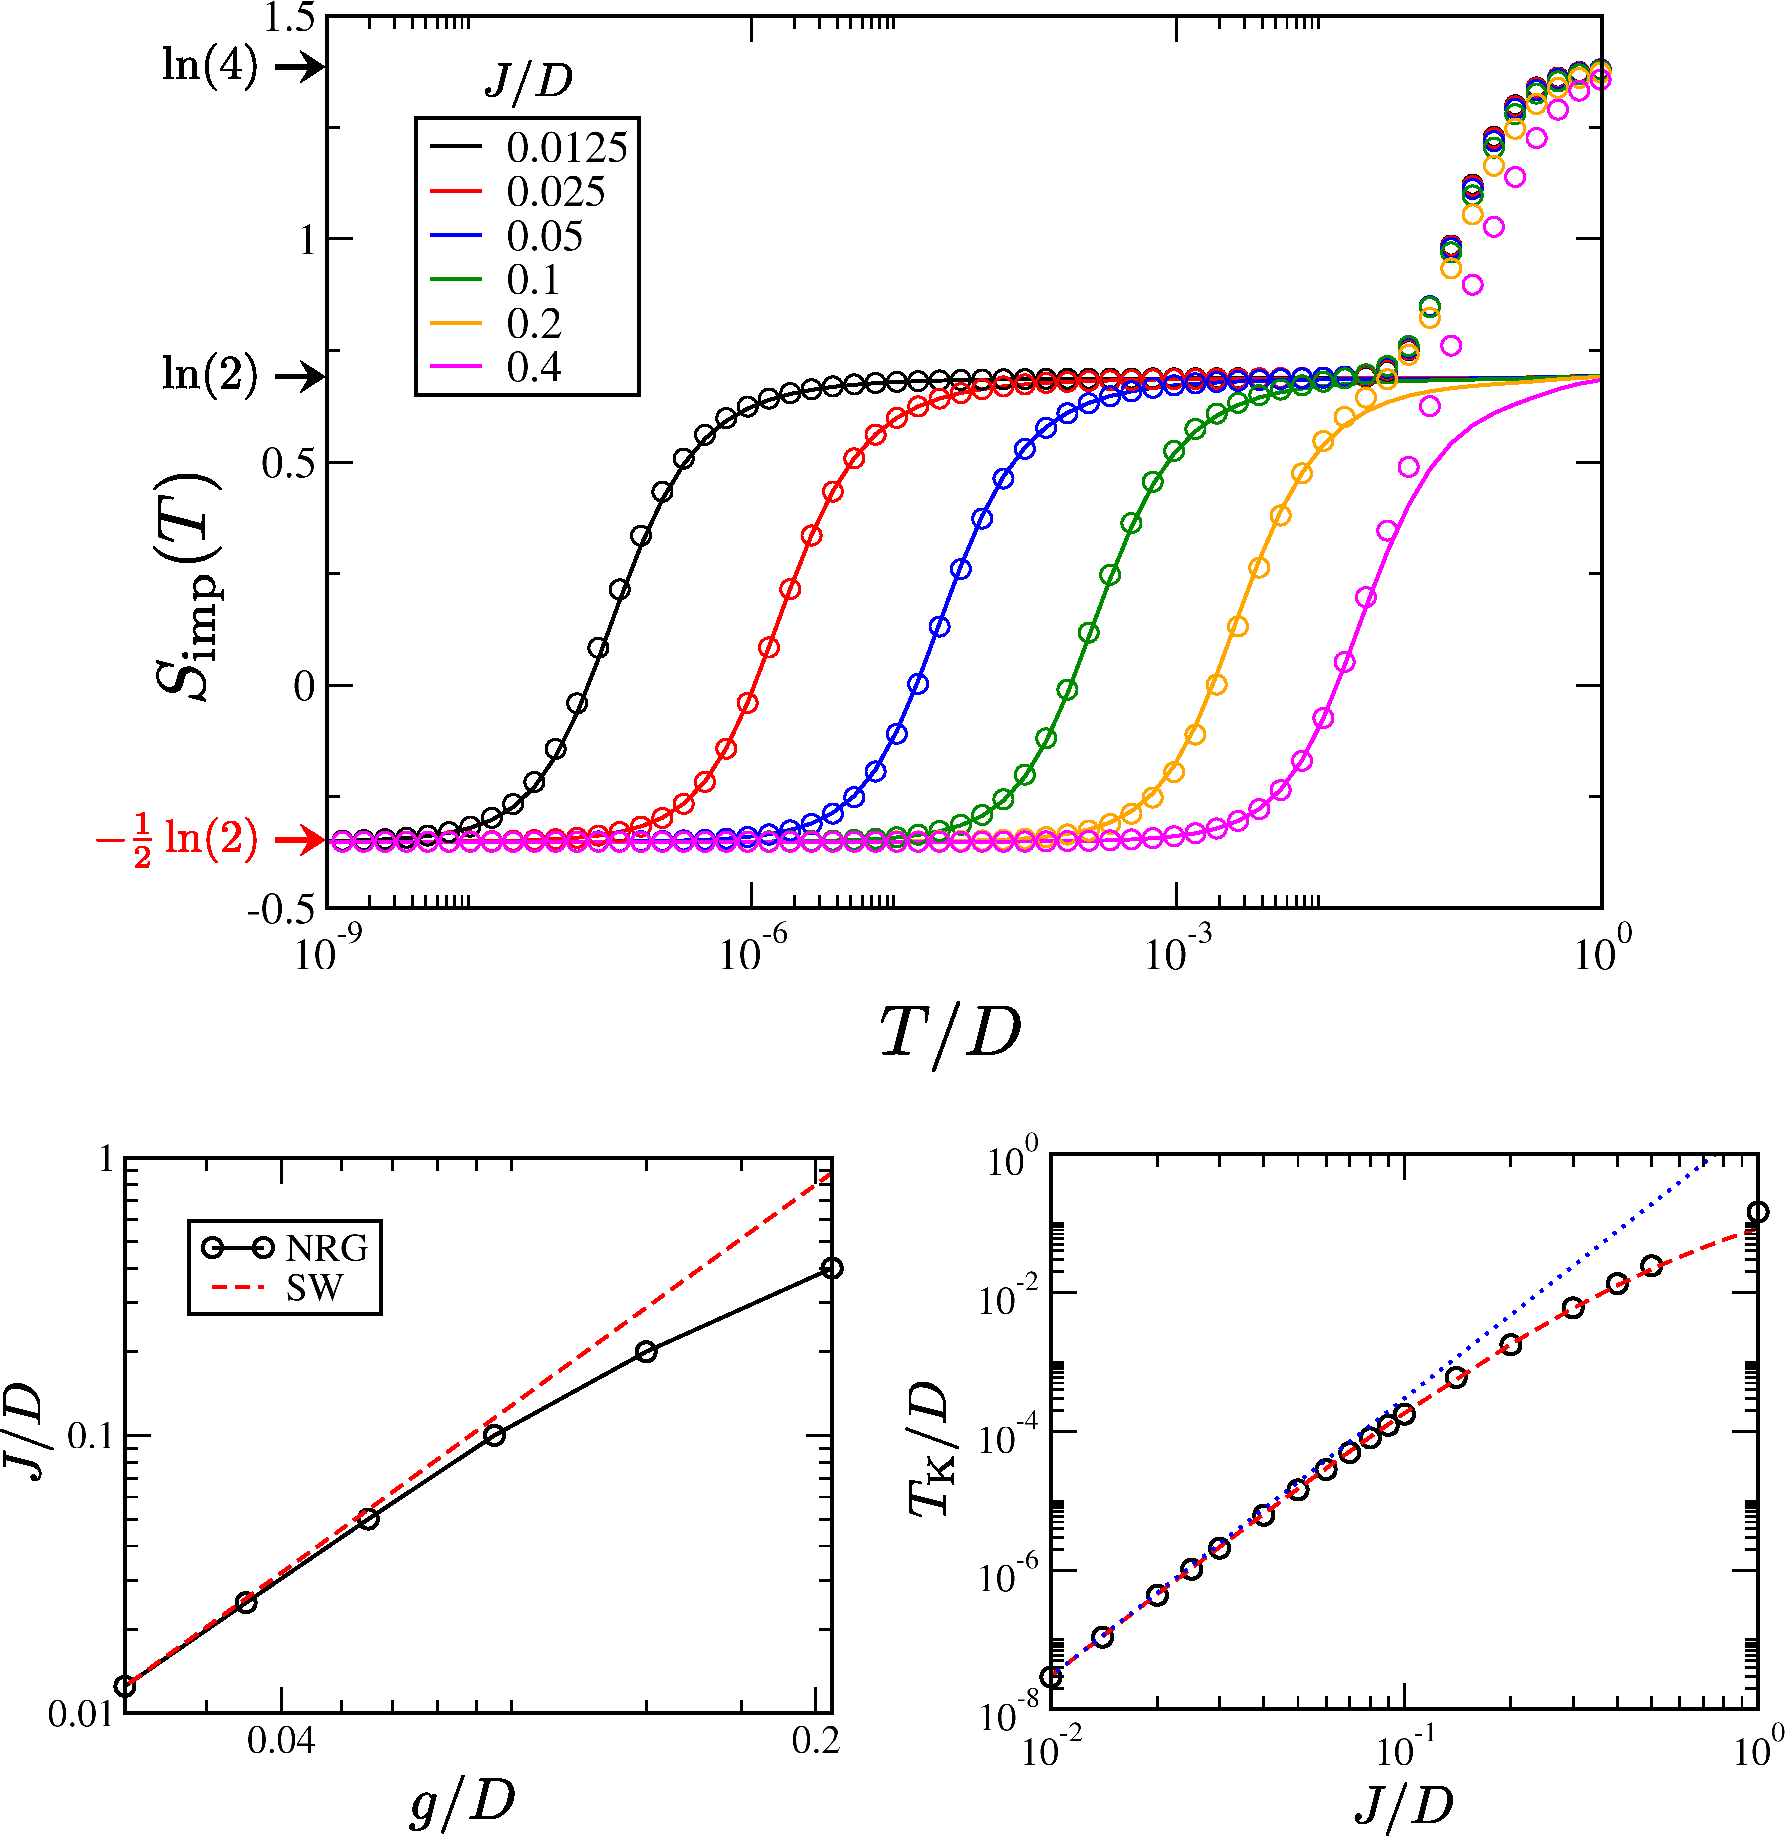
\includegraphics[width = 0.8\linewidth]{figures/chapter2/kondo2.pdf}
	\caption{
		% \justifying
		  NRG results for an impurity embedded in magic angle TBG. Main panel: Entropy $S_{\rm imp}$ vs $T$ for Anderson and Kondo impurities (points and lines respectively)  for different impurity-host couplings. For a given Kondo $J$, the low temperature physics of an Anderson model with fixed $U=0.4D$ is fit by tuning $g$. The relationship between $J$ and $g$ is shown in the lower-left inset (points), comparing with the SW result (red dashed line). The evolution of $T_K$ with $J$ is shown in the lower-right inset (points), comparing with Eq.~\ref{eq:tkHO} (red dashed line) and its small-$J$ asymptote (blue dotted line). \rev{$T_K$ is extracted numerically from NRG results for the entropy, defined in practice via $S_{\rm imp}(T=T_K)=0$.}}
	\label{fig:kondomagic}
\end{figure}

In Fig.~\ref{fig:kondomagic} we turn to an analysis of NRG results for systems at the magic angle itself. In the main panel (top) we plot the impurity entropy $S_{\rm imp}(T)$ for impurities of either Anderson type (Eq.~\ref{eq:AM}, points) or Kondo type (Eq.~\ref{eq:KM}, lines), for different impurity-host couplings. 

At the highest temperatures $T\sim D$, the Anderson impurity again shows $\ln(4)$ entropy for the four quasi-degenerate impurity states. At lower temperatures $T\sim U$, the charge configurations on the impurity in the Anderson model are frozen out and only the local moment spin states survive, giving $\ln(2)$ entropy. In this regime the system is close to the LM fixed point. RG flow towards the ${\rm SSC}_{\rm HO}$ strong coupling fixed point results in a crossover in the entropy on the scale of the Kondo temperature $T\sim T_K$ to $S_{\rm imp}=-\tfrac{1}{2}\ln(2)$. This remains the $T=0$ residual impurity entropy for TBG systems at the magic angle. However, the Kondo scale itself varies with the impurity-host coupling, as seen in the main panel of Fig.~\ref{fig:kondomagic} by the evolution of the different lines. For good scale separation $T_K\ll U$, we see clear two-stage behavior, with distinct crossovers to and from the LM fixed point in the Anderson model. However, given the strongly enhanced $T_K$ at the magic angle, such a scale separation may not be in evidence in practice (see e.g.~pink and orange lines in Fig.~\ref{fig:kondomagic} which show a more or less direct crossover in the entropy from $\ln(4)$ to $-\tfrac{1}{2}\ln(2)$; or indeed the cases close to the magic angle in Fig.~\ref{fig:angles}).

By contrast, the Kondo impurity features only the local moment spin configurations and hence has a $\ln(2)$ entropy at high temperatures $T\sim D$. The Kondo scale generated by finite antiferromagnetic exchange coupling $J$ results in the same crossover to the ${\rm SSC}_{\rm HO}$ fixed point, with the same $T=0$ residual entropy of $-\tfrac{1}{2}\ln(2)$. Indeed, RG arguments imply~\cite{Hewson} that the physics of the Anderson and Kondo models for $T\ll U$ should be identical, providing the effective Kondo coupling $J$ is chosen appropriately for a given $U$ and $g$ of the Anderson model. To verify this Anderson-Kondo mapping in the magic-angle TBG setting, in Fig.~\ref{fig:kondomagic} we considered Kondo models with different $J$ and then fit Anderson models to match the low-temperature physics by tuning $g$ at fixed $U$. In such a way, the Kondo and Anderson models have the same Kondo temperature $T_K$.  The precise agreement in the universal regime confirms that at particle-hole symmetry the effective Kondo model is a faithful description of the more microscopic Anderson model. 

The Anderson-Kondo mapping can be performed perturbatively via the approximate SW transformation \cite{Hewson,schrieffer1966relation} as described in Sec.~\ref{sec:Kondo}. 
The exact relationship between $J$ and $g$ as extracted from our NRG results is shown in the lower left panel of Fig.~\ref{fig:kondomagic} as the circle points. The SW result (red dashed line) is seen to work well when the bare coupling of the underlying Anderson model is small, $g\ll U$  (small $T_K$ regime). Away from this limit, NRG results show that the Kondo model is still the correct low-energy effective model, but that non-perturbative techniques must be used to obtain the correct effective model parameters~\cite{rigo2020machine}. The evolution of the numerically-extracted Kondo temperature as a function of the effective $J$ is shown in the lower right panel of Fig.~\ref{fig:kondomagic} (points), and is compared with the analytic result for the Kondo model Eq.~\ref{eq:tkHO}
(red dashed line). The blue dotted line is the asymptotic small-$J$ limit of this expression, $T_K \sim (4\rho_0 J)^{1/\alpha}$.

Our full NRG results for an impurity in magic angle TBG therefore confirm the analytic predictions of the previous sections. For a comparison with results for an impurity coupled to a standard logarithmic vHs, see Appendix~\ref{app:KondoC}.

\rev{Finally, we comment on the role of potential scattering and particle-hole symmetry breaking. In the above analysis we have for simplicity neglected particle-hole asymmetry in the TBG host DoS by employing the symmetric BM model. However, we believe this approximation is well-justified and does not affect the presented results. Although in principle particle-hole asymmetry can lead to Kondo screening in the linear pseudogap case \cite{Fritz2013} relevant to the low-energy Dirac cone in TBG away from the magic angle, the singlet-doublet quantum phase transition arises only at very strong asymmetry. In practice, the relatively small particle-hole symmetry breaking in TBG means that the impurity problem is far away from the asymmetric strong coupling Kondo phase. Within the doublet local moment phase, particle-hole asymmetry is RG irrelevant and can be safely ignored. We have also assumed that the impurity itself is particle-hole symmetric ($\epsilon_d=-U_d/2$ in the Anderson model, or $V=0$ in the Kondo model). Relaxing this condition induces potential scattering in the TBG host. Very strong deviations away from the half-filled Anderson impurity are required to destroy the local moment ground state (the resulting asymmetric Kondo strong coupling state is continuously connected to the trivial empty orbital state of the impurity). In this regime, the mapping to the Kondo model breaks down (the large value of $V$ in the Kondo model required for Kondo screening is unphysical). Therefore, we argue that the results presented above are generic for a local moment impurity embedded in a TBG host material.}

%############


\section{Conclusions}
\label{sec:conclusions}
In this paper, we have studied the physics of a single magnetic impurity in TBG at, and close to, the magic angle. We find a surprisingly rich range of behavior, rooted in the unique evolution of the TBG density of states. It is interesting to note that there is no Kondo screened ground state in general, only at the magic angle. However, the signatures at finite temperature relevant to experiment show highly nontrivial structure due to the interplay between van Hove and Dirac physics on the level of a strongly correlated quantum impurity problem. Close to the magic angle, the TBG host density of states at different energy scales yields different limits of paradigmatic Kondo models -- from logarithmic and power-law diverging Kondo to pseudogap vanishing Kondo. The subtle renormalization group flow between these limits shows up in the temperature and energy dependence of physical observables.

The behavior we uncover should be detectable in STM experiments. Indeed we argue that the impurity response in TBG gives a very clear signature of magic angle physics. Magnetic impurities may therefore prove useful as highly sensitive \textit{in-situ} probes for moir\'{e} materials.

An interesting direction of future research is the role of the RKKY interaction between multiple magnetic impurities in TBG, and how it competes with the Kondo effect of individual impurities near the magic angle.

\rev{Although van Hove-boosted Kondo physics may be observable in other systems (including 3d bulk metals \cite{igoshev2019giant,igoshev2022giant} with magnetic impurities), we note that TBG stands out as a uniquely tunable platform. Furthermore, TBG also allows one to study the complex interplay of these effects with Dirac physics.}

%%%%%%%%%%%%%%%

\section*{Acknowledgments}
	We thank S.~Polla, V.~Cheianov, L.~Classen, A.~Chubukov, and L.~Fu for helpful discussions. this work is part of the D-ITP consortium,
	a program of the Netherlands Organisation for Scientific Research (NWO) that is funded by the Dutch Ministry of Education, Culture and Science (OCW). DOO acknowledges the support from the Netherlands Organization for Scientific Research (NWO/OCW) and from the European Research Council (ERC) under the European Union's Horizon 2020 research and innovation programme. AKM acknowledges funding from the Irish Research Council through the Laureate Award 2017/2018 grant IRCLA/2017/169.

%##################

% \appendix
\newpage
\section{Appendix}
\subsection{Locating saddle point positions in the particle-hole symmetric BM model}
\label{app:KondoA}
To locate the saddle points in the Brillouin  zone, we require gradients of the energy. The flat bands make it imperative that the first derivative is computed very accurately, and this means that we must avoid crude finite difference methods for numerical derivatives of the energy. This problem can be addressed by utilizing our analytical access to the Hamiltonian itself, and implementing the Hellman-Feynman theorem,
\begin{equation}
	\pdv{E}{k^i} = \expval{\pdv{H}{k^i}}{\psi_k}, 
\end{equation}
where $\psi_k$ is the wavefunction of the lowest positive energy band at momentum $\vec{k}$. A more extended analysis of this method has been introduced recently in \cite{chandrasekaran2022detect}.

The saddle point is found by minimizing the value of $\left(\partial_{k_x} \epsilon_\vec{k}\right)^2 + \left(\partial_{k_y} \epsilon_\vec{k}\right)^2$ over the Brillouin  zone vectors, by using the conjugate gradient method.
The coefficients for the local energy dispersion are then calculated along the principal directions of the saddle point. These directions are given by the eigenvectors of the Hessian matrix, and are in general different from the $k_x$ and $k_y$ of the Brillouin  zone. Derivatives are convenient to compute along the natural Brillouin  zone directions, however. The trick to overcome this is to note that a matrix formed from $n$ derivatives of a scalar transforms like a rank-$n$ tensor. Then the tensor transformation rule can be used with a covariant Jacobian to obtain the coefficients along the rotated axes. 

One subtlety is that for angles very close to the magic angle, there are secondary vHs points at other locations in the Brillouin zone than those indicated in Fig.~\ref{fig:contourslog}. For the purposes of the Kondo effect, we have only considered the one with the largest spectral weight, since this is found to dominate the results of our NRG calculations. This is done by computing the local dispersion coefficients $\alpha$ and $\beta$ at each of the saddle points, and picking the one with the largest value of $\frac{1}{\sqrt{\alpha\beta}}$. 

%!!!!!!!!!!!!



%###############
\newpage
\subsection{Mapping from TBG density of states to the NRG Wilson chain}
\label{app:KondoB}
The TBG DoS away from the magic angle has two qualitative features: the linear-pseudogap Dirac cone at low energies and the divergence due to the vHs on the scale of $E_v$. We extract an effective model DoS from analysis of the BM model for different twist angles -- see left panels of Fig.~\ref{fig:wc} for the cases explicitly considered in the main text (we have rescaled the energy range in terms of the bandwidth cutoff and normalized the spectrum to unity). This DoS is then discretized logarithmically and mapped to a Wilson chain \cite{bulla2008numerical} as described in Sec.~\ref{subsec:nrg}. The corresponding Wilson chain hopping parameters are plotted in the right panels of Fig.~\ref{fig:wc}. The results show that the different DoS elements can be captured in NRG through the crossover behavior in the functional form of the Wilson chain.
\begin{figure}[H]
	\centering
	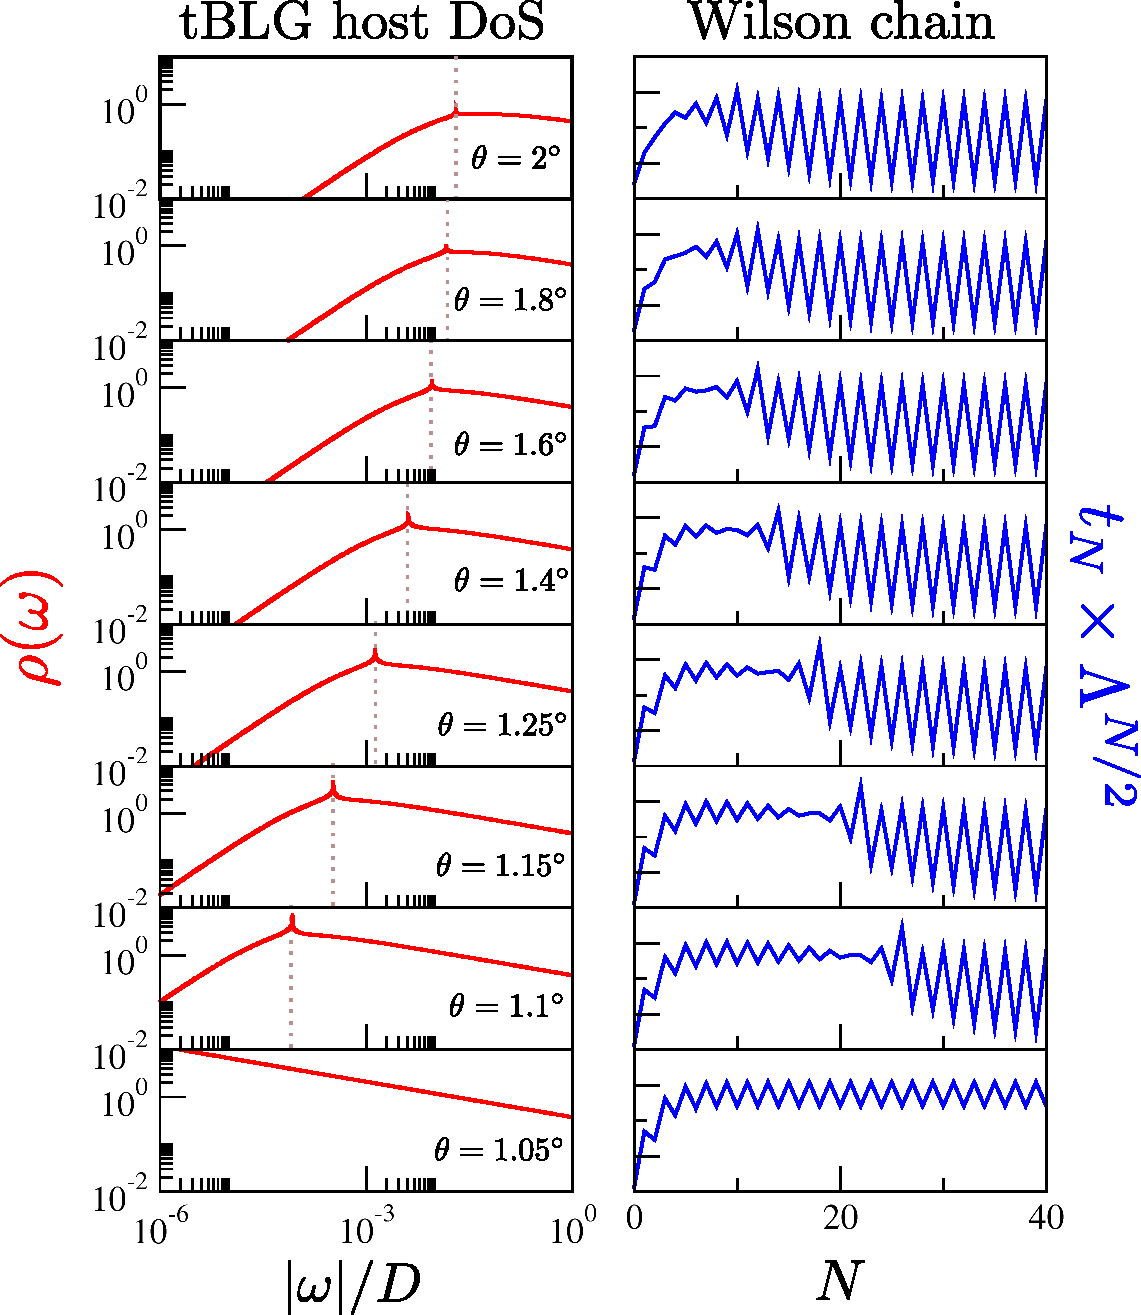
\includegraphics[width = 0.8\linewidth]{figures/chapter2/DoS_wc_labels.pdf}
	\caption{
		%\justifying
		  Left panels: DoS used in our NRG calculations, obtained from analysis of the effective BM model, for different twist angles $\theta$ as used in the main text. Vertical dotted lines show the $E_v$ scale at which the vHs divergence occurs. This scale moves to lower energies as the magic angle is approached. Right panels: corresponding Wilson chain coefficients.}
	\label{fig:wc}
\end{figure}



%##################
\newpage
\subsection{NRG calculations for an impurity coupled to a conventional log-vHs host}
\label{app:KondoC}
In Fig.~\ref{fig:Slog} we provide reference NRG calculations for a Kondo impurity coupled to a pure log-diverging DoS. This gives a useful comparison to our result for an impurity embedded in the magic-angle TBG system, which has a HO-vHs point and hence a stronger power-law diverging DoS. As predicted from our perturbative scaling (poor man's scaling) results, the system flows towards strong coupling in all cases, in which the impurity is Kondo-screened. The residual entropy at $T=0$ is seen to be $S_{\rm imp}=0$, although this limit is approached logarithmically slowly from below. This is characteristic of the logarithmic DoS. From the scaling with bare coupling strength $J$ in the left panel, the Kondo temperature $T_K$ is seen to be enhanced relative to the metallic case, but substantially suppressed relative to the power-law diverging DoS case. In the right panel, we analyze the behavior of $T_K$ in more detail, comparing NRG results at different $J$ (circle points) with our analytic formula Eq.~\ref{eq:TKLog} (black line). The results agree almost perfectly. The red dashed line is the asymptotic result at small $J$, which also does remarkably well compared with exact NRG results.
\begin{figure}[H]
	\centering
	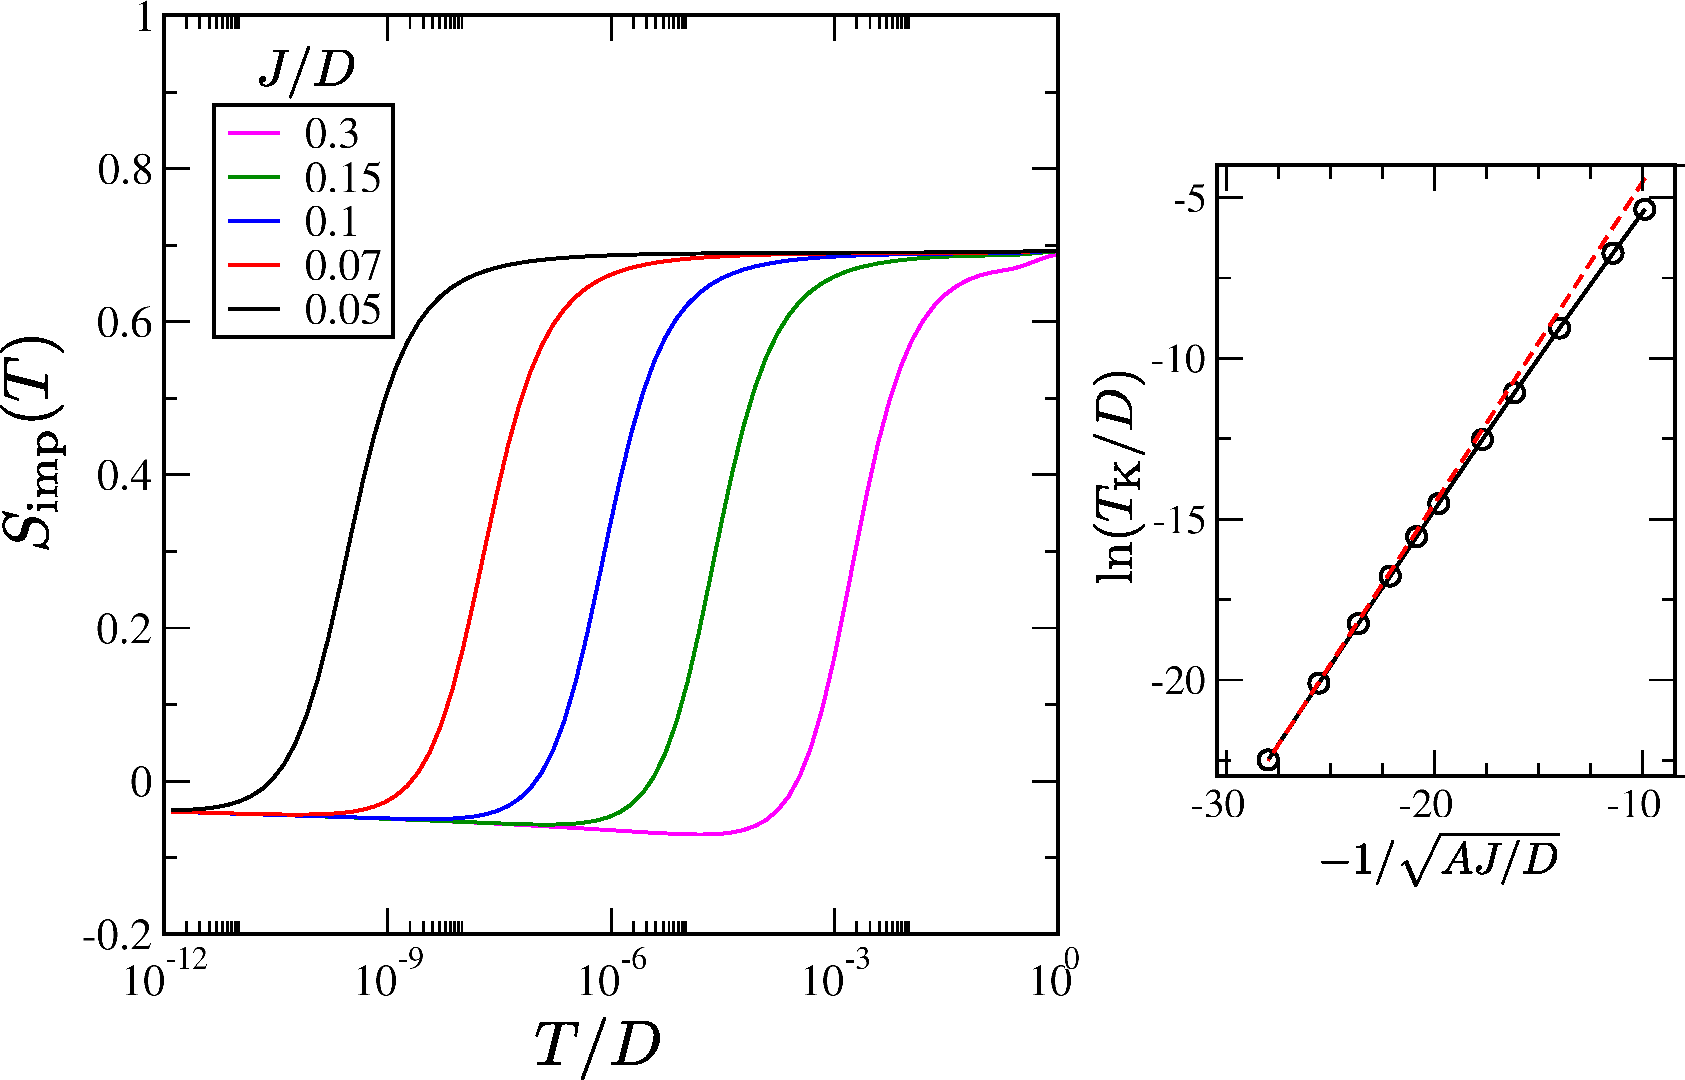
\includegraphics[width = \linewidth]{figures/chapter2/Slog_labels.pdf}
	\caption{
		% \justifying
		  Main panel: NRG results for the impurity entropy $S_{\rm imp}$ vs temperature $T$ for different bare coupling strengths $J$, in a system with a pure log-diverging DoS (standard vHs). Right inset shows the extracted $T_K$ scale (points), compared with Eq.~\ref{eq:TKLog} (black line) and the asymptotic result $T_K \sim D e^{-1/\sqrt{A J/D}}$ (red dashed line), with $A=a\rho_0 D/2$.}
	\label{fig:Slog}
\end{figure}



%####################

		% \chapter{Lyapunov Exponents in the bipartite SYK model]}
\label{ch:LyapbSYK}

\section*{Attribution}
This paper has been previously published in Physical review D under the title \textbf{\textit{Lyapunov exponents in a Sachdev-Ye-Kitaev-type model with population imbalance in the conformal limit and beyond}}, together with Mikael Fremling, Stephan Plugge and Lars Fritz~\cite{shankar2023lyapunov}.

\section*{Abstract}
The Sachdev-Ye-Kitaev (SYK) model shows chaotic behavior with a maximal Lyapunov exponent. In this paper, we investigate the four-point function of a SYK-type model numerically, which gives us access to its Lyapunov exponent. The model consists of two sets of Majorana fermions, called A and B, and the interactions are restricted to being exclusively pairwise between the two sets, not within the sets. We find that the Lyapunov exponent is still maximal at strong coupling. Furthermore, we show that even though the conformal dimensions of the A and B fermions change with the population ratio, the Lyapunov exponent remains constant, not just in the conformal limit where it is maximal, but also in the intermediate and weak coupling regimes.

\section{Introduction}
Over the last decade, the Sachdev-Ye-Kitaev (SYK) model has been established as a paradigmatic model accounting for a variety of phenomena ranging from aspects of the physics of black holes to non-Fermi liquids~\cite{Chowdhury-RMP2022,Rosenhaus2019-review,Franz2018-review,patel_quantum_2017,tikhanovskaya2022maximal}.
There exist two main variants of this model in the literature: one that is formulated in terms of $N$ 'complex' Dirac fermions,
and another one written in terms of $N$ 'real' Majorana fermions.
In both cases, the fermions interact via random four-body terms.
Irrespective of the formulation, one of the main features of the model is that it exhibits emergent conformal symmetry in the infrared in the strong-coupling and large-$N$ limit.
The scaling dimension of the fermion correlation function is given by $\Delta = \frac{1}{4}$ \cite{maldacena_comments_2016,polchinski_spectrum_2016},
indicative of strong interactions (for comparison, a free fermion has scaling dimension $1/2$). 

There has been a variety of proposals for the creation of SYK-like models in laboratory setups.
They range from mesoscopic systems hosting Majorana modes~\cite{Pikulin2017,Chew2017},
or Dirac fermions in graphene flakes~\cite{Chen2018,can_charge_2019},
to ultracold atomic systems \cite{danshita2017creating,wei2021optical}.
A comprehensive review of such possible setups can be found in Refs.~\cite{Chowdhury-RMP2022,Franz2018-review} and references therein.


\begin{figure}[h]
	\centering
	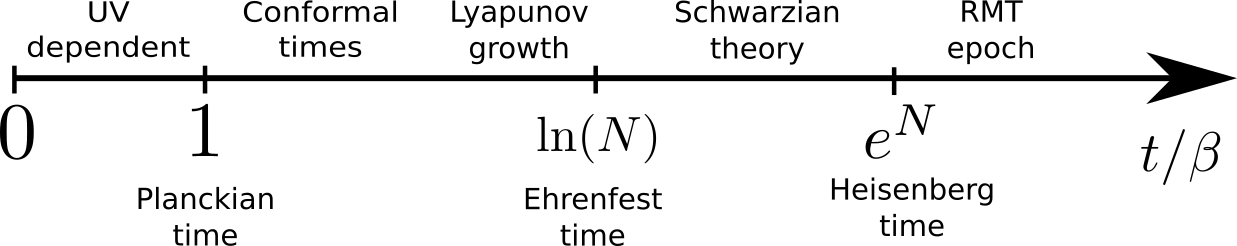
\includegraphics[width=1.0\columnwidth]{figures/chapter1/TimeLine.png}
	\caption{The SYK model exhibits multiple characteristic timescales, and with that associated regimes of dynamics.
		Crucial quantities in distinguishing the different limits are the number of fermions $N$ and coupling strength $\beta J$.
		This paper studies the region characterized by Lyapunov growth.
	}
	\label{fig:TimeLine}
\end{figure}

The SYK model involves three important time scales, as shown in Fig.~\ref{fig:TimeLine} (henceforth,
we measure time $t$ in units of $\beta$ and set $\hbar=k_b=1$).
They are called the Planckian time~\cite{Zaanen2019,hartnoll2021planckian,patel_magnetotransport_2018,hartnoll2022colloquium}, $t_P$,
the Ehrenfest time~\cite{gu2019relation,larkin1969quasiclassical,hashimoto_out--time-order_2017,kobrin_many-body_2021,craps_lyapunov_2020}, $t_E$,
and the Heisenberg time $t_H$. The shortest time scale, $t_P$,
is set by the condition $t_P/\beta\approx 1$. For times shorter than $t_P$,
we expect non-universal physics determined by processes at the cutoff scale.
For $t_P<t<t_E$, the dynamics is governed by the conformal mean-field theory.
The chaotic behavior associated with Lyapunov growth~\cite{stanford_many-body_2016,maldacena_bound_2016} in this regime is due to leading irrelevant operators of order $1/N$ beyond mean-field.
The Ehrenfest time is given as $t_E/\beta \approx \ln N$, where $N$ is the number of fermions.
The dynamical behavior for $t_E<t<t_H$ ceases to be described by mean-field theory plus corrections and the associated description is in terms of the Schwarzian theory of black holes.
Eventually, there is the Heisenberg time, $t_H/\beta \approx e^N$.
For times longer than $t_H$, the dynamics is described by random matrix theory. 

In this paper we study a related model, introduced in Ref.~\cite{Fremling_2022,fremling_bipartite_2021}, which emerges as a Majorana variant of the SYK model. 
It is called the bipartite SYK (or b-SYK) model and, as explained in Sec.~\ref{sec_model},
can be seen as a restricted version of the standard SYK model. Incidentally,
Majorana or complex fermion versions of similar models also appear as a natural way to incorporate internal symmetries in SYK models~\cite{lantagne2020diagnosing,Kim2019,sahoo_traversable_2020},
or to couple two or more SYK models~\cite{chowdhury_translationally_2018}.
We are interested in times shorter than the Ehrenfest time $t_E$, and mostly focus on the chaotic behavior. Furthermore, we are interested in studying the growth of the four-point function not just in the full conformal limit at strong coupling, but also at intermediate and weak couplings, as these might be relevant for experimentally achievable values of coupling and temperature, as the b-SYK model has been shown to be realizable in a laboratory by straining a real material in Ref.\cite{fremling_bipartite_2021}.
%

We show that the Lyapunov exponent is maximal in the conformal limit, just as for the SYK model~\cite{stanford_many-body_2016,maldacena_bound_2016,maldacena_comments_2016}. The behavior of the chaos exponent for a general number of majorana fermions in the $A$ and $B$ subsets of the b-SYK at finite coupling is unanswered in the existing literature and is the subject of the present study.
We use numerical methods to solve the Schwinger-Dyson and Bethe-Salpeter equations that are needed to extract the Green functions and Lyapunov exponents, respectively.
We find that the b-SYK model ratio of $A$ and $B$ majoranas does not influence the Lyapunov exponent for all values of coupling.



The present paper is organized as follows:
In Sec.~\ref{sec_model}, we introduce the b-SYK model and comment on how it is related to more common variants of SYK models.
In Sec.~\ref{sec_greens} we discuss the two-point functions in and away from the conformal limit. In Sec.~\ref{sec_four_point},
we compute the four-point function and introduce the equations that allow us to extract the Lyapunov exponents. In Sec.~\ref{sec_Results},
we numerically find the Lyapunov exponents and show how they depend on the population balance between $A$ and $B$ Majorana fermions.



\section{Model and methods}\label{sec_model}

\subsection{The bipartite SYK model}

The bipartite SYK (b-SYK) model consists of two sets of Majorana fermions, labelled $A$ and $B$,
with random interactions between pairs of $A$ and pairs of $B$ fermions.
Interactions between only $A$ or only $B$ fermions are absent,
and the fermion parity in both the $A$ and $B$ subsets is conserved.
The Hamiltonian reads
%
\begin{equation}
	H = \frac{1}{4}\sum_{ij,\alpha\beta}J_{ij\alpha\beta}\gamma^A_i\gamma^A_j \gamma^B_\alpha \gamma^B_\beta~.
\end{equation}
%
To distinguish the two sets of fermions we use latin indices $i,j$ for the $A$-flavor Majorana fermions ($\gamma_i^A$),
and greek indices $\alpha,\beta$ for $B$-flavor Majorana fermions ($\gamma_\alpha^B$).

We allow for $N_A$ Majorana fermions of the $A$-type and $N_B$ of the $B$-type.
The ratio $\kappa=N_A/N_B$ accounts for the relative size of the two sets.
The couplings $J_{ij\alpha\beta}$ are random and only act between sets, not within each set.
Concerning the normalization of the interaction strength, we follow the convention of Gross and Rosenhaus~\cite{gross_generalization_2017} and choose the variance of the coupling constant to be~\footnote {note that this is the $q=2, f=2$ limit of Ref.~\cite{gross_generalization_2017}}
%
\[
\langle J_{ij\alpha\beta} J_{i^{\prime}j^{\prime}\alpha^{\prime}\beta^{\prime}}\rangle=
\frac{J^2(N_A+N_B)}{N_A^2N_B^2}\delta_{i,i^{\prime}}\delta_{j,j^{\prime}}\delta_{\alpha,\alpha^{\prime}}\delta_{\beta,\beta^{\prime}}.
\] 

In this work, we will define $N$ as the geometric mean of $N_A$ and $N_B$, $N=\sqrt{N_{A}N_{B}}$.
We can then rewrite $\frac{N_A+N_B}{N_A^2N_B^2}=(\sqrt{\kappa} + \frac{1}{\sqrt{\kappa}})/N^3$,
which makes the symmetry between $\kappa$ and $1/\kappa$ apparent.
For clarity, this convention differs from the one used in Refs.~\cite{Fremling_2022,fremling_bipartite_2021}, where 
%
$
\langle J_{ij\alpha\beta} J_{i^{\prime}j^{\prime}\alpha^{\prime}\beta^{\prime}}\rangle=
\frac{J^2}{2\sqrt{N_A N_B}^3}\delta_{i,i^{\prime}}\delta_{i,i^{\prime}}\delta_{j,j^{\prime}}\delta_{\alpha,\alpha^{\prime}}\delta_{\beta,\beta^{\prime}}\;.$



The model has a well-defined large-$N$ conformal limit upon taking $N_A,N_B\to\infty$, keeping the ratio $\kappa = \frac{N_A}{N_B}$ fixed.
Rather than a single scaling dimension as in the standard SYK model, the two sets of Majorana fermions,
$A$ and $B$, have distinct scaling dimensions, $\Delta_A$ and $\Delta_B$.
These depend on the parameter $\kappa$, cf. Ref.~\cite{Fremling_2022}, as
%
\begin{equation} \label{eq_scalin_dims}
	\kappa = \frac{2 \Delta_A}{1-2\Delta_A}\left( \frac{1}{\tan \left( \pi \Delta_A\right)}\right)^2.
\end{equation}
%
For $\kappa=1$ we find $\Delta_A=\Delta_B=1/4$, just like in the standard SYK model,
although the model is still different since not all Majorana fermions interact with each other.
For other values of $\kappa$, both scaling dimensions interpolate between $0$ and $1/2$ while always fulfilling $\Delta_A+\Delta_B=1/2$.
Tunable scaling dimensions have also been found in other variants of the SYK model e.g Ref.~\cite{Marcus2019,Kim2019,garcia-garcia_sparse_2021,xu_sparse_2020}.




\subsection{Schwinger-Dyson equations}
\label{sec_greens}
%
For the later numerical analysis to follow, one main input is required, the Green functions.
Hence we recapitulate the crucial steps in solving the model in the large-$N$ limit via the associated Schwinger-Dyson equations.
For more details on the procedure in the present context see e.g.~Ref.~\cite{Fremling_2022}. In this part of the paper,
the focus is more on finding a reliable numerical implementation of the Green function that allows to access the conformal limit. 
The crucial step is to consider the mean-field or large-$N$ limit.
Compared to the conventional SYK model, we have to modify the limit slightly.
We take $N_A,N_B\to\infty$ while keeping $\kappa=N_a/N_B$ fixed. As in the conventional case,
there is one order $O(1)$ diagram per species of fermions, the so-called 'melon' diagrams.
These are shown in Fig.~\ref{fig:GreensFunction}.
The diagrams contain the coupling $J^2$ to all orders and exhibit an emergent conformal symmetry in the infrared, as explained below.

\begin{figure}
	\centering
	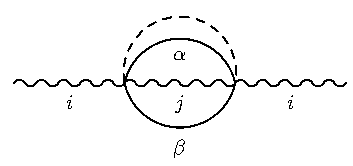
\includegraphics[width=0.8\columnwidth]{figures/chapter1/GA.pdf}
	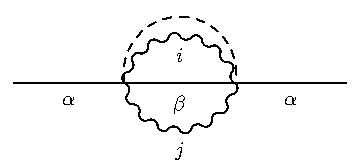
\includegraphics[width=0.8\columnwidth]{figures/chapter1/GB.pdf}
	\caption{The diagrams that contribute to the self energies of A (top) and B (bottom) Majoranas in the large-$N$ limit. Wiggly (solid) lines denote A (B) Majorana propagators,
		and the dotted line indicates a quenched disorder average $\sim J^2$.}
	\label{fig:GreensFunction}
\end{figure}


\subsubsection{Imaginary time formalism}
\label{sec:imaginary_time}
%
The discussion of equilibrium properties of the Schwinger-Dyson (SD) equations is easiest carried out in the finite-temperature imaginary time formalism.
The inverse temperature is denoted as $\beta =1/T$ ($\hbar=k_B=1$).
For the two species, the SD equations read
%
\begin{equation}
	G^{A/B}(\i\omega_n) = \frac{1}{-\i\omega_n - \Sigma^{A/B}(\i\omega_n)},
	\label{eq:SDeqns}
\end{equation}
%
where the respective self energies are given by 
%
\begin{subequations}
	\begin{align}
		\Sigma_A(\tau) &= \frac{J^2}2(1+\frac 1\kappa)\, G^A(\tau) \left(G^B(\tau)\right)^2, \\
		\Sigma_B (\tau)&= \frac{J^2}2(1+\kappa)\, G^B(\tau) \left( G^A(\tau)\right)^2 \;.
	\end{align}
	\label{eq:bSYK_Equations}
\end{subequations}
%
Here $\omega_n=(2n+1)\pi T$ for integer $n$ are the fermionic Matsubara frequencies, whereas $\tau$ denotes imaginary time. 
The Fourier transform  between Matsubara frequencies and imaginary time is defined according to 
%
\begin{subequations}
	\begin{align}
		G(\i\omega_n) &= \int_0^\beta e^{\i\omega_n \tau} G(\tau) \, d\tau \;,\label{eq:time2freq}\\
		G(\tau) &= \frac{1}{\beta} \sum_{\omega_n} e^{-\i\omega_n \tau} G(\i\omega_n)\;. \label{eq:freq2time} 
	\end{align}
\end{subequations}
%
One can show analytically that the finite temperature imaginary time Green functions are given by~\cite{Fremling_2022}
%
\begin{eqnarray}\label{eq_finiteTanaly}
	G^{A}(\tau)&=&a \; \sgn(\tau) \left(  \frac{\pi}{\beta \sin\left(\frac{\pi \tau}{\beta} \right)}\right)^{2\Delta_A}\;,\nonumber \\
	G^{B}(\tau)&=&b\;  \sgn(\tau) \left(  \frac{\pi}{\beta \sin\left(\frac{\pi \tau}{\beta} \right)}\right)^{2\Delta_B}\;,
\end{eqnarray}
%
where for a given $\kappa$, the scaling dimensions $\Delta_A$ and $\Delta_B$ are related according to Eq.~\eqref{eq_scalin_dims}.

As far as the overall constants $a$ and $b$ are concerned, it is found that only the product $ab$ is uniquely determined, and not the numbers $a$ and $b$ themselves. When we assume that the self energy dominates over the free propagator, we can use the conformal ansatz in equations Eq.~\eqref{eq:bSYK_Equations} and ~\eqref{eq:SDeqns} for each of the $A$ and $B$ flavors respectively. Naively, we would expect that the two equations are sufficient to constrain the two unknowns $a$ and $b$ respectively, but it turns out the two equations are identical, and only the product is constrained. The result is 
\begin{align}
	\frac{1}{a^2 b^2} &= \frac{J^2}{2}\left(1+\frac{1}{\kappa}\right) 2\pi \frac{\cot(\pi\Delta_A)}{1-2\Delta_A} \\
	&= \frac{J^2}{2}\left(1+\kappa\right) 2\pi \frac{\cot(\pi\Delta_B)}{1-2\Delta_B} .
\end{align} 
However, in the real system, at short times, the conformal ansatz is no longer valid, and the free propagator wins over, and $G^{A/B}(\tau)$ should go as $\frac{1}{2}\sgn(\tau)$. This is sufficient to uniquely constrain the short time dynamics of the model. 

Numerically, we solve the Schwinger-Dyson equations in a self-consistent manner by repeated evaluation of the Green functions and self-energies paired with an iteration on an imaginary time grid running from $0$ to $\beta$. Eqs.~\eqref{eq:time2freq},
\eqref{eq:freq2time} and similarly for the self-energies here are recast in the form of discrete Fourier transforms,
for which there are efficient numerical algorithms such as Fast Fourier transform.
To achieve convergence, we use a weighted update of the Green functions according to $G^{new} = \frac{x}{-\i\omega_n - \Sigma} + (1-x)G^{old}$ with a small mixing parameter $x$; here $\Sigma(\i\omega_n)$ denotes the associated self-energy calculated from $G^{old}$ of the previous iteration.

In Fig.~\ref{fig_G_tau} we show the Majorana Green functions $G^{A/B}(\tau)$ for $\beta J=10$ and for a variety of values of $\kappa$.
By fitting the numerically obtained $G^{A/B}$ to Eq.~\eqref{eq_finiteTanaly} one can see that the scaling dimensions indeed match the conformal results. Overall,
we find excellent agreement in the region $0\ll\tau\ll\beta$.


\begin{figure}
	{\centering
		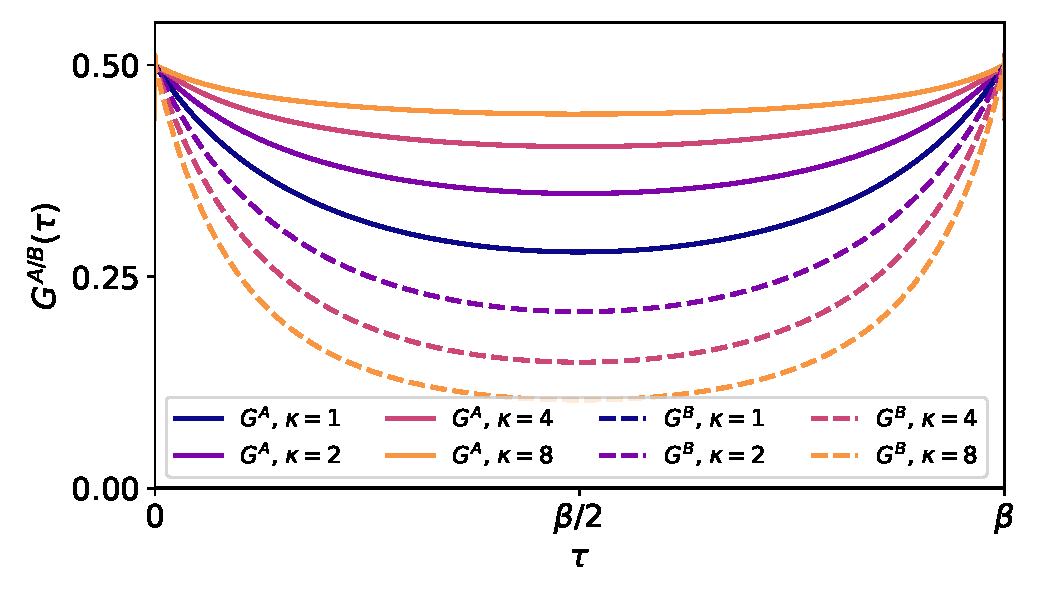
\includegraphics[width=1.00\columnwidth]{figures/chapter1/G_tau.pdf} 
		\caption{Finite temperature Majorana Green functions $G^{A/B}(\tau)$ for $\beta J=10$ and several values of $\kappa$.
			Taking $\kappa\to 1/\kappa$ exchanges the $A$ and $B$ species, hence we plot only $\kappa\geq1$.
			\label{fig_G_tau}}}
\end{figure}




\subsection{Real time formalism}
\label{sec:Real_Time}


The main goal of this paper is to numerically study the out-of-time-ordered correlator (OTOC) in the b-SYK model.
To compute it, we need the real time retarded Green function as input.
We first note the Dyson equation for the retarded propagator ~\cite{parcollet_non-fermi-liquid_1999,lantagne2020diagnosing,sahoo_traversable_2020,gu_notes_2020}
%
\begin{equation}
	\left(G^R (\omega+\i\delta)\right)^{-1} = \omega+\i\delta - \Sigma^R(\omega+\i\delta).
	\label{eq:retarded_dyson_equation}
\end{equation}
%
We drop the $A/B$ labels, unless explicitly required. The spectral decomposition for the Green functions reads: 
%
\begin{subequations}
	\label{eq:SpectralDecomposition}
	\begin{align}
		G(z) &= \int_{-\infty}^\infty \, \frac{d\Omega}{\pi}\frac{\rho(\Omega)}{z-\Omega},\label{eq:HilbertTransform} \\
		\rho(\omega) &= -\Im{G^R(\omega+\i\delta)}\;. \label{eq:spectraldef}
	\end{align}
\end{subequations}
%

\begin{figure*}
	{\centering
		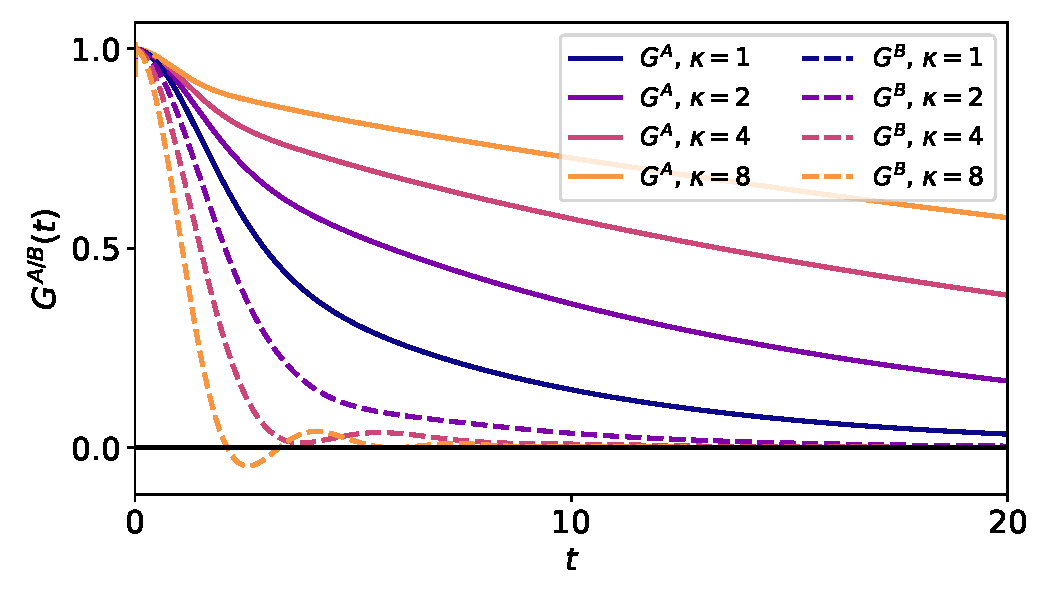
\includegraphics[width=0.49\linewidth]{figures/chapter1/G_t.pdf}
		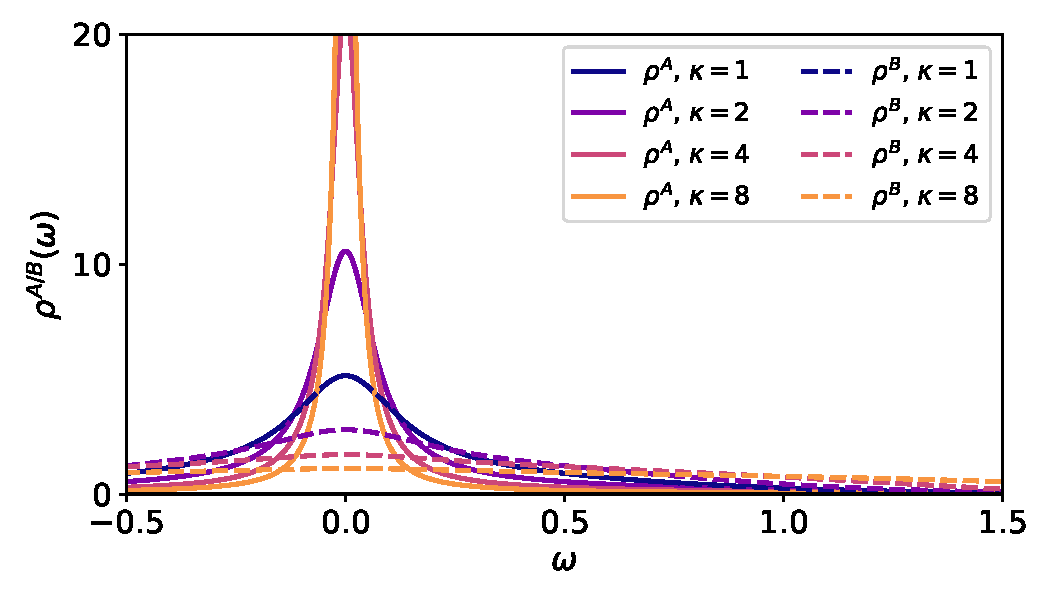
\includegraphics[width=0.49\linewidth]{figures/chapter1/rho_w.pdf} 
		\caption{
			\emph{Left panel}:
			the retarded Green functions $G_R^{A/B}(t)$ for $\beta J = 10$.
			The characteristic decay time-scale is set by the conformal dimension $\Delta_{A,B}$.
			\\\emph{Right panel}: the corresponding spectral functions, showing a strong dependence on $\kappa$.
			\label{fig_G_t}}}
\end{figure*}
%
Since the self energies are well defined in imaginary time according to Eq.~\eqref{eq:bSYK_Equations}, we can use Eqs.~\eqref{eq:time2freq},
\eqref{eq:freq2time} and \eqref{eq:SpectralDecomposition} to express $\Sigma(\i\omega_n)$ in terms of the spectral function.
The analytical continuation is then done by replacing $\i\omega_n \xrightarrow{} \omega+\i\delta$, resulting in
%
\begin{equation}
		\Sigma^R_B(\omega+i\delta) = \frac{J^2}2(1+\kappa) \int\int\int
		\frac{\dd \omega_1}{\pi} \frac{\dd \omega_2}{\pi}\frac{\dd \omega_3}{\pi}
		\rho_A(\omega_1)\rho_A(\omega_2)\rho_B(\omega_3)
		\frac{\left[n(\omega_1)n(\omega_2)n(\omega_3) + n(-\omega_1)n(-\omega_2)n(-\omega_3)\right]}{\omega + \i\delta -\omega_1 -\omega_2-\omega_3},
\end{equation}
%
where $n(\omega)$ is the Fermi-Dirac distribution function.
The expression for $\Sigma_A$ is obtained by changing $A\leftrightarrow B$, and $\kappa\leftrightarrow 1/\kappa$.
In principle,
the Schwinger-Dyson equations can be solved iteratively for $G^R_{A/B}(\omega)$ and $\rho^{A/B}(\omega)$.
However, nested numerical integration is both highly inefficient in its usage of resources and numerically unstable.
Instead, it is beneficial to rewrite it using the following decomposition which allows an implementation using only the discrete Fourier transform, cf. Refs.~\cite{Plugge2020,sahoo_traversable_2020}.
We can express the self energies as
%
\begin{align}
		\Sigma^R_A(\omega+\i\delta) &=  \begin{multlined}[t][] -\imath \frac{J^2}2(1+\frac1\kappa)\int_0^\infty dt\,
			e^{\i(\omega+\i\delta)t}
			\left[n^+_A(t)n^+_B(t)n^+_B(t) + n^-_A(t)n^-_B(t)n^-_B(t)\right] \end{multlined}\\
		\Sigma^R_B(\omega+\i\delta) &= \begin{multlined}[t][] -\imath \frac{J^2}2(1+\kappa)\int_0^\infty dt\,
			e^{\i(\omega+\i\delta)t}
			\left[n^+_B(t)n^+_A(t)n^+_A(t) + n^-_B(t)n^-_A(t)n^-_A(t)\right]\end{multlined}\;,
\end{align}
%
where the function $n^{\pm}_{A/B}(t)$ is defined through
%
\begin{align}
	n^{\pm}_{A/B}(t) = \int_{-\infty}^\infty \frac{d\omega_1}{\pi} e^{-\i\omega_1t}\rho_{A/B}(\omega_1)n(\pm\omega_1)\;.
\end{align}


The retarded Green function and the corresponding spectral functions obtained from the real-time/frequency iteration of the above SD equations are shown in Figure~\ref{fig_G_t}.


\section{The four-point function}\label{sec_four_point}

We now turn our attention to the four-point correlators of the b-SYK model,
and in particular to the out-of-time-ordered correlators (OTOCs).
Before we have a look into OTOCs themselves, we first discuss conventional four-point functions. In imaginary time,
a general four-point function of Majoranas has the form~\cite{gross_generalization_2017} 
%
\begin{equation}\label{eq:fourpoint}
	\mathcal{F}(\tau_1,\tau_2,\tau_3,\tau_4) = \frac{1}{N^2}\sum_{ijkl}\expval{\gamma^{f_1}_i(\tau_1)\gamma^{f_2}_j(\tau_2),\gamma^{f_3}_k(\tau_3)\gamma^{f_4}_l(\tau_4)}.
\end{equation}
%
The disorder averaging and the large-$N$ limit taken together restrict the contributions to the four-point functions to stem from what are known as ladder diagrams. These can be categorized into four channels,
depending on the flavors of the incoming and outgoing pairs of fermion propagators: AA-AA, AA-BB, BB-AA, and BB-BB.
A diagram with $n+1$ rungs can be obtained from a diagram with $n$ rungs by convolution with a kernel~\cite{stanford_many-body_2016}. In the vicinity of the Ehrenfest time $t_E$,
this can be cast as a self-consistent Bethe-Salpeter equation according to
%
\begin{equation}
		\mathcal{F}_{\alpha\beta}(\tau_1,\tau_2,\tau_3,\tau_4) = \int \dd \tau \dd \tau^\prime \,K_{\alpha\gamma}(\tau_1,\tau_2,\tau,\tau^\prime)\, \mathcal{F}_{\gamma\beta}(\tau,\tau^\prime,\tau_3,\tau_4)
		\label{eq:kernelmatrixequation}
\end{equation}
	where $\gamma$ is summed over, and the Kernel matrix is given as (in imaginary time and a regularized version in real time respectively)
	\begin{align}
		K_{\alpha\gamma}(\tau_1\cdots \tau_4) = -J^2
		\begin{pmatrix}
			\frac{1}{2} (1+\frac{1}{\kappa})\,G^A(\tau_{13})G^A(\tau_{24})\left(G^B(\tau_{34})\right)^2   & (1+\frac{1}{\kappa})\,G^A(\tau_{13})G^A(\tau_{24})\left(G^A(\tau_{34})G^B(\tau_{34})\right) \\ 
			(1+\kappa) \,G^B(\tau_{13})G^B(\tau_{24})\left(G^A(\tau_{34})G^B(\tau_{34})\right) & \frac{1}{2} (1+\kappa)\, G^B(\tau_{13})G^B(\tau_{24})\left(G^A(\tau_{34})\right)^2
		\end{pmatrix} 
		\label{eq:kernel_tau} \\
		K^R_{\alpha\gamma}(t_1\cdots t_4) = J^2
		\begin{pmatrix}
			\frac{1}{2} (1+\frac{1}{\kappa})\,G^A_R(t_{13})G^A_R(t_{24})\left(G^B_W(t_{34})\right)^2   & (1+\frac{1}{\kappa})\,G^A_R(t_{13})G^A_R(t_{24})\left(G^A_W(t_{34})G^B_W(t_{34})\right) \\ 
			(1+\kappa) \,G^B_R(t_{13})G^B_R(t_{24})\left(G^A_W(\tau_{34})G^B_W(t_{34})\right) & \frac{1}{2} (1+\kappa)\, G^B_R(t_{13})G^B_R(t_{24})\left(G^A_W(t_{34})\right)^2
			\label{Kernelt}
		\end{pmatrix}
	\end{align}
The indices $\alpha,\beta,\gamma$ refer to the flavors of the Majorana propagators on the external legs. For example,
$F_{00}$ refers to the AA-AA scattering and $F_{10}$ refers to BB-AA scattering. 
A diagrammatic representation of the matrix-kernel equation~\eqref{eq:kernelmatrixequation} is shown in Fig.~\ref{fig:diagrammatic_kernel}.


\begin{figure*}
	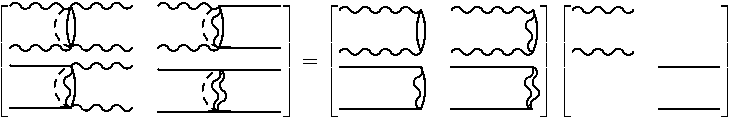
\includegraphics[width=1.0\linewidth]{figures/chapter1/CompiledMatrixDiagram.pdf}
	\caption{Diagrammatic representation of the matrix-kernel equation~\eqref{eq:kernelmatrixequation} at first order. Repeated application of the kernel $K$ generates all terms in $\mathcal F$}
	\label{fig:diagrammatic_kernel}
\end{figure*}

%
Quantum chaos is characterized by the Lyapunov exponent. Instead of looking at the real time version of Eq.~\eqref{eq:fourpoint}, we consider a regularized version according to
%
\begin{equation}
	F_{ab}(t_1,t_2) = \frac{1}{N^2}\sum_{a,b}\overline{\Tr{\sqrt{\rho}\comm{\gamma_a(t_1)}{\gamma_b(0)}\sqrt{\rho}\comm{\gamma_a(t_2)}{\gamma_b(0)}}}. 
	\label{eq:regularized_OTOC}
\end{equation}
%
This regularized OTOC has the thermal density matrix $\rho$ of the thermal average split evenly between pairs of Majorana operators, and brackets $[\cdot,\cdot]$ denote commutators.
In diagrammatic language this means that the four point function is evaluated on a double-fold Schwinger-Keldysh contour with insertions of the Majorana operators as shown in Fig.~\ref{fig:two_fold_contour}.
%

\begin{figure}
	\centering
	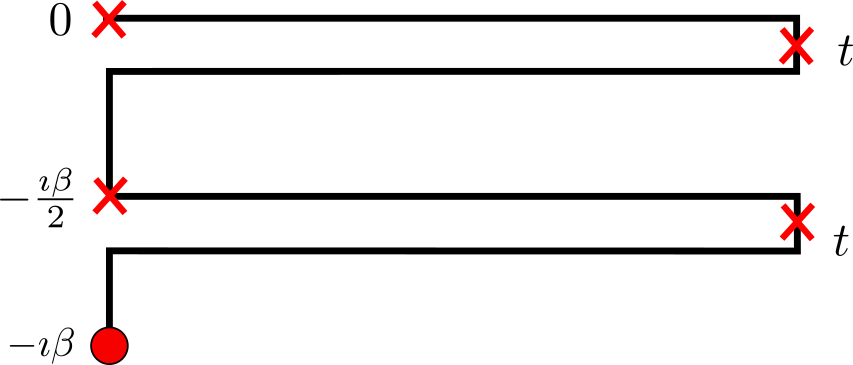
\includegraphics[width=1.0\columnwidth]{figures/chapter1/TwoFoldCountour.png}
	
	\caption{Schwinger-Keldysh contour with two temporal folds (excursions to time $t$) and Majorana operator insertions (red crosses) that represents the regularized OTOC in Eq.~\eqref{eq:regularized_OTOC}.}
	\label{fig:two_fold_contour}
\end{figure}
%
This is a regularization not of the UV, but of the IR. Details on which of the many possible choices of regularization and Schwinger-Keldysh contour one might pick can be found in Ref.~\cite{romero2019regularization}.
The key point is that for massless theories, which the SYK universality class belongs to,
all different regularizations give the same exponential growth, even though the values of the actual OTOCs may differ.
For the choice in Eq.~\eqref{eq:regularized_OTOC}, the four point function in question will be generated by ladder diagrams with retarded or advanced Green functions on the rails,
and so-called Wightman functions $G^W(t)=G(\frac{\beta}{2} + i t)$ on the rungs.
Formally, the latter are obtained by an analytic continuation of the imaginary time Green function noted in Sec.~\ref{sec:imaginary_time}.
This analytic continuation can be be performed with the use of the spectral decomposition, also known as a Hilbert transform.
In total, one obtains the result
\begin{equation}
	G^W(\omega) = \frac{\rho(\omega)}{2\cosh{\frac{\beta\omega}{2}}}.
\end{equation}



The late time exponential growth of the OTOC \cite{maldacena_bound_2016} can then be fit to the Lyapunov ansatz
%
\begin{equation}
	\mathcal{F}_{\alpha\beta}(t_1,t_2) = e^{\lambda_{\alpha\beta}\frac{(t_1 + t_2)}{2}}\, f_{\alpha\beta}(t_{12})\;.
	\label{eq:Lyapunov_Ansatz}
\end{equation}
%
As opposed to the standard SYK model, each of the four different scattering channels might ostensibly have its own Lyapunov exponent. It turns out that this is not the case.
A detailed technical explanation involving the consistency of the Lyapunov ansatz with a single exponent $\lambda$ is presented in Appendix~\ref{sec:technical_explanation}. 

A simple qualitative argument for a single Lyapunov exponent is that the scattering channels all feed back into each other.
The AA-AA scattering amplitude also passes through the AA-BB channel and then back into the BB-AA channel.
This imposes a sense of self-consistency between the scattering channels,
which in turn forces them to have the same late time Lyapunov growth.

\subsection{Conformal limit}
Taking the ansatz that all four Lyapunov exponents $\lambda_{\alpha\beta}$ are the same, {\it i.e.} $\lambda_{\alpha \beta}=\lambda$ allows us to make an ansatz for the growth equation. First, we will notice that the equations for $f_{00}$ and $f_{10}$ decouple, and we get the same equations for the other pair $f_{01}$ and $f_{11}$. 
In the conformal limit, following~\cite{maldacena_comments_2016} we can use the conformal mapping to obtain the retarded and Wightman Green functions from Eqs.~\eqref{eq_finiteTanaly} to get
\begin{subequations}
	\label{eq:ConfRealTimeGreens}
	\begin{align}
		G_R^A(t) &= 2 a \cos(\pi \Delta_{A})\left(\frac{\pi}{\beta \sinh\frac{\pi t}{\beta}}\right)^{2\Delta_{A}} \\
		G_W^A(t) &= a \left(\frac{\pi}{\beta\cosh\frac{\pi t}{\beta}}\right)^{2\Delta_A}, 
	\end{align}
\end{subequations}
and likewise for the $B-$ fermions. 
The growth ansatz can also be made in analogy with the regular SYK case: 
\begin{equation}
	\begin{pmatrix}
		f_{00}(t_{12}) \\ f_{10}(t_{12}) 
	\end{pmatrix}
	= \begin{pmatrix}
		a\,\mathcal{C}_a\left(\frac{\pi}{\beta\cosh{(t_{12}\frac{\pi}{\beta
				})}}\right)^{2\Delta_a + h} \\
		b\,\mathcal{C}_b\left(\frac{\pi}{\beta\cosh({t_{12}\frac{\pi}{\beta
			}})}\right)^{2\Delta_b + h}
	\end{pmatrix} e^{h(t_1+t_2)\frac{\pi}{\beta
	}} \label{eq:b-sykLyapunovAnsatz}
\end{equation}
It can be noted that Eq.~\eqref{eq:b-sykLyapunovAnsatz} is a way of rewriting Eq.~\eqref{eq:Lyapunov_Ansatz} in a way that is convenient for the conformal limit calculation. $\mathcal{C}_a $ and $ \mathcal{C}_b$ are hitherto undetermined constants. The equations one needs to solve are then (the factors of $\frac{\pi}{\beta}$ have been chosen appropriately so that they scale away) 
	\begin{subequations}
		\begin{multline}
			e^{h(t_1 + t_2)} f_{00}(t_{12}) = \frac{J^2}{2}(1+\frac{1}{\kappa})\int dt_3 dt_4 \biggl[G^A_R(t_{13})G^A_R(t_{24})G^B_W(t_{34})^2f_{00}(t_{34}) + \\2 G^A_R(t_{13})G^A_R(t_{24})G^B_W(t_{34})G^A_W(t_{34})f_{10}(t_{34})\biggr]e^{h(t_3+t_4)}
		\end{multline}
		\begin{multline}
			e^{h(t_1 + t_2)} f_{10}(t_{12}) = \frac{J^2}{2}(1+\kappa)\int dt_3 dt_4 \biggl[G^B_R(t_{13})G^B_R(t_{24})G^A_W(t_{34})G^B_W(t_{34})f_{00}(t_{34}) + \\2 G^B_R(t_{13})G^B_R(t_{24})G^A_W(t_{34})^2f_{10}(t_{34})\biggr]e^{h(t_3+t_4)}
		\end{multline}
	\end{subequations}
The way to solve these equations is to first represent the $t_{34}$ part as an inverse fourier transform, which factorizes the integral into a function that depends only on $t_3$ and another function that depends only on $t_4$, which can be separately integrated. One can express the fourier transforms for powers of hyperbolic sines and cosines as analytic continuations of the Euler Beta function 
\begin{subequations}
	\begin{align}
		\int_{-\infty}^\infty dt\,e^{i\omega t} \frac{1}{(\cosh{t})^\alpha} &=  2^{\alpha-1} \mathrm{B}\left(\frac{\alpha - i\omega}{2},\frac{\alpha + i\omega}{2}\right) ,\\
		\int_{-\infty}^\infty dt\,e^{i\omega t} \frac{\theta(t)}{(\sinh{t})^\alpha} &=  2^{\alpha-1}\mathrm{B}\left(\frac{\alpha - i\omega}{2},1-\alpha\right) .
	\end{align}
\end{subequations}
The result then is that  
\begin{subequations}
	\begin{align}
		\mathcal{C}_a &= \mathcal{M}\left(\mathcal{C}_a + 2\mathcal{C}_b\right) \\
		\mathcal{C}_b &= \mathcal{M}^\prime\left(2\mathcal{C}_a + \mathcal{C}_b\right) ,
	\end{align}
	\label{eq:confomalconsistency}
\end{subequations}

where 
\begin{align}
	\mathcal{M} &= \frac{(1-2\Delta_A)\sin(2\pi\Delta_A)}{\pi}\frac{(\Gamma(1-2\Delta_A))^2\Gamma(2\Delta_A + h)}{\Gamma(2-2\Delta_A + h)} \\
	\mathcal{M}^\prime &= \frac{(1-2\Delta_B)\sin(2\pi\Delta_B)}{\pi}\frac{(\Gamma(1-2\Delta_B))^2\Gamma(2\Delta_B + h)}{\Gamma(2-2\Delta_B + h)}
\end{align}
The equations Eqs.~\eqref{eq:confomalconsistency} only have a trivial solution $\mathcal{C}_A = \mathcal{C}_B = 0$ if either of the scaling dimensions are $0$ or $\frac{1}{2}$, i.e, the $\kappa = 0$ and $\kappa \rightarrow \infty$ models are not chaotic in the strictly conformal limit. 

For any other intermediate $\kappa$, even infinitesimally small, Eqs.~\eqref{eq:confomalconsistency} permit a solution if 
\begin{align}
	\det\mqty[\mathcal{M}-1 & 2\mathcal{M} \\
	2\mathcal{M}^\prime & \mathcal{M}^\prime -1] = 0. 
\end{align}
We have solved this equation for $h$ and the solution found is always $h=1$ for any value of $\kappa$. This means that for the b-SYK model, it is always possible to increase the coupling and lower the temperature sufficiently that the system always has a maximal Lyapunov exponent $\lambda = \frac{2\pi}{\beta}$. 

For realistic couplings and not too low temperatures, one needs to observe the behavior of the Lyapunov exponent including non-conformal corrections to the Green function by perturbatively including the $\i\omega$ term in the Dyson equation.  If the correction to the Kernel is $\delta K_R$, and if we compute all the eigenvalues in the conformal limit and call them $k(h)$, the we can Taylor-expand $k(h)$ about $h=1$. The point is now that $h=1$ gives eigenvalue $k(h) = 1$, so we say that 
\begin{align}
	k(1+\delta h) = 1 + k^\prime(1) \, \delta h 
\end{align}
Thus in order to keep the kernel having eigenvalue 1, the correction 
\begin{align}
	\expval{\delta K_R} &= \delta h k^\prime(1) \nonumber\\
	\implies \delta h &= \frac{\expval{\delta K_R}}{ k^\prime(1)}
\end{align}
is the first non-conformal correction to the lyapunov exponent.


\subsection{Numerical analysis for weak and intermediate coupling}

Rather than take this complicated approach, the weak and intermediate coupling limits can be analysed numerically.
We can bring the kernel equation into the concise form 
%
\begin{align}
	f_{\alpha\beta}(\omega) = \abs{G^\alpha_R(\omega+\i\frac{\lambda}{2})}^2\left(\tilde{K}_{\alpha 0} \ast f_{0\beta} + \tilde{K}_{\alpha 1}\ast f_{1\beta}\right)~,
	\label{eq:conv_form}
\end{align} 
%
where additionally a Fourier transform was performed. The ansatz function $f_{\alpha\beta}(\omega')$ is analyzed in frequency space, see below.
We also denote the shifted frequency $\tilde{\omega} = \omega + \i\frac{\lambda}{2}$ that enters in the retarded Green function.
The latter is obtained from the regular retarded Green function $G_R(\omega+\i\delta)$ that is calculated in Sec.~\ref{sec:Real_Time} by use of the Fourier shift theorem.
The symbol $\star$ in Eq.~\eqref{eq:conv_form} indicates a convolution with the ansatz function $f_{\gamma\beta}(\omega)$.
The part of the kernel elements $\tilde{K}_{\alpha\gamma}(\omega)$ that contains the Wightman Green functions is given by 
%
	\begin{equation}
		\tilde{K}_{\alpha\beta}(\omega) = J^2
		\begin{pmatrix}
			\frac{1}{2} (1+\frac{1}{\kappa})\,\mathfrak{F}\left[(G^B_W(t))^2\right] & (1+\frac{1}{\kappa})\,\mathfrak{F}\left[(G^B_W(t)\,G^A_W(t))\right]  \\
			(1+\kappa)\,\mathfrak{F}\left[(G^B_W(t)\,G^A_W(t))\right]  & \frac{1}{2}(1+\kappa)\,\mathfrak{F}\left[(G^A_W(t))^2\right]
		\end{pmatrix}
	\end{equation}

%
where $\mathfrak{F}\left[ \cdot \right] $ represents the Fourier transformation.


Finally, note that Eq.~\eqref{eq:conv_form} can be thought of as an eigenvalue problem for the ansatz $f_{\alpha\beta}(\omega)$ in frequency space $\omega$ with a block structure $\alpha,\beta$ due to the different kernel matrix blocks according to 
%

	\begin{equation}
		\begin{bmatrix}
			f_{00}(\omega)\\
			f_{10}(\omega)\\
			f_{01}(\omega)\\
			f_{11}(\omega)
		\end{bmatrix}=\begin{bmatrix}
			|G_{R}^{A}(\tilde{\omega})|^{2}\tilde{K}_{00}(\omega-\omega^{\prime}) & |G_{R}^{A}(\tilde{\omega})|^{2}\tilde{K}_{01}(\omega-\omega^{\prime}) & 0 & 0 \\
			|G_{R}^{B}(\tilde{\omega})|^{2}\tilde{K}_{10}(\omega-\omega^{\prime}) & |G_{R}^{B}(\tilde{\omega})|^{2}\tilde{K}_{11}(\omega-\omega^{\prime}) & 0 & 0 \\
			0 & 0 &
			|G_{R}^{A}(\tilde{\omega})|^{2}\tilde{K}_{00}(\omega-\omega^{\prime}) & |G_{R}^{A}(\tilde{\omega})|^{2}\tilde{K}_{01}(\omega-\omega^{\prime})\\
			0 & 0 &
			|G_{R}^{B}(\tilde{\omega})|^{2}\tilde{K}_{10}(\omega-\omega^{\prime}) & |G_{R}^{B}(\tilde{\omega})|^{2}\tilde{K}_{11}(\omega-\omega^{\prime})
		\end{bmatrix}\begin{bmatrix}f_{00}(\omega^{\prime})\\
			f_{10}(\omega^{\prime})\\
			f_{01}(\omega^{\prime})\\
			f_{11}(\omega^{\prime})
		\end{bmatrix}\;.
	\end{equation}
%
On the finite frequency grid, the convolution operations naturally translate to matrix multiplications.
For a solution of $f_{\alpha\beta}$ to exist, the matrix operator needs to have $1$ as its largest eigenvalue~\cite{stanford_many-body_2016,maldacena_comments_2016,gu2019relation}.
This is equivalent to saying that Eq.~\eqref{eq:Lyapunov_Ansatz} is the correct form for the late time behavior of the OTOC,
and the Lyapunov exponent is thus fixed uniquely. 
%
\begin{figure*}
	%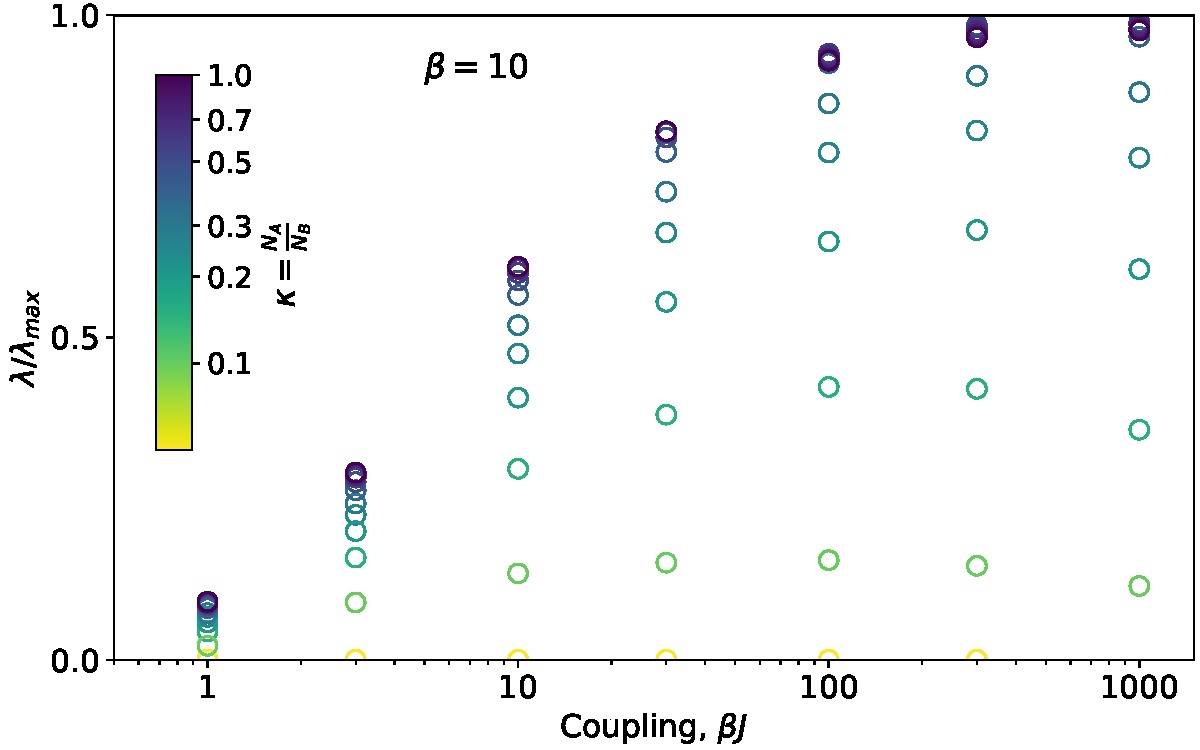
\includegraphics[width=1.00\columnwidth]{pic/bSYK_Lyaponov.pdf}
	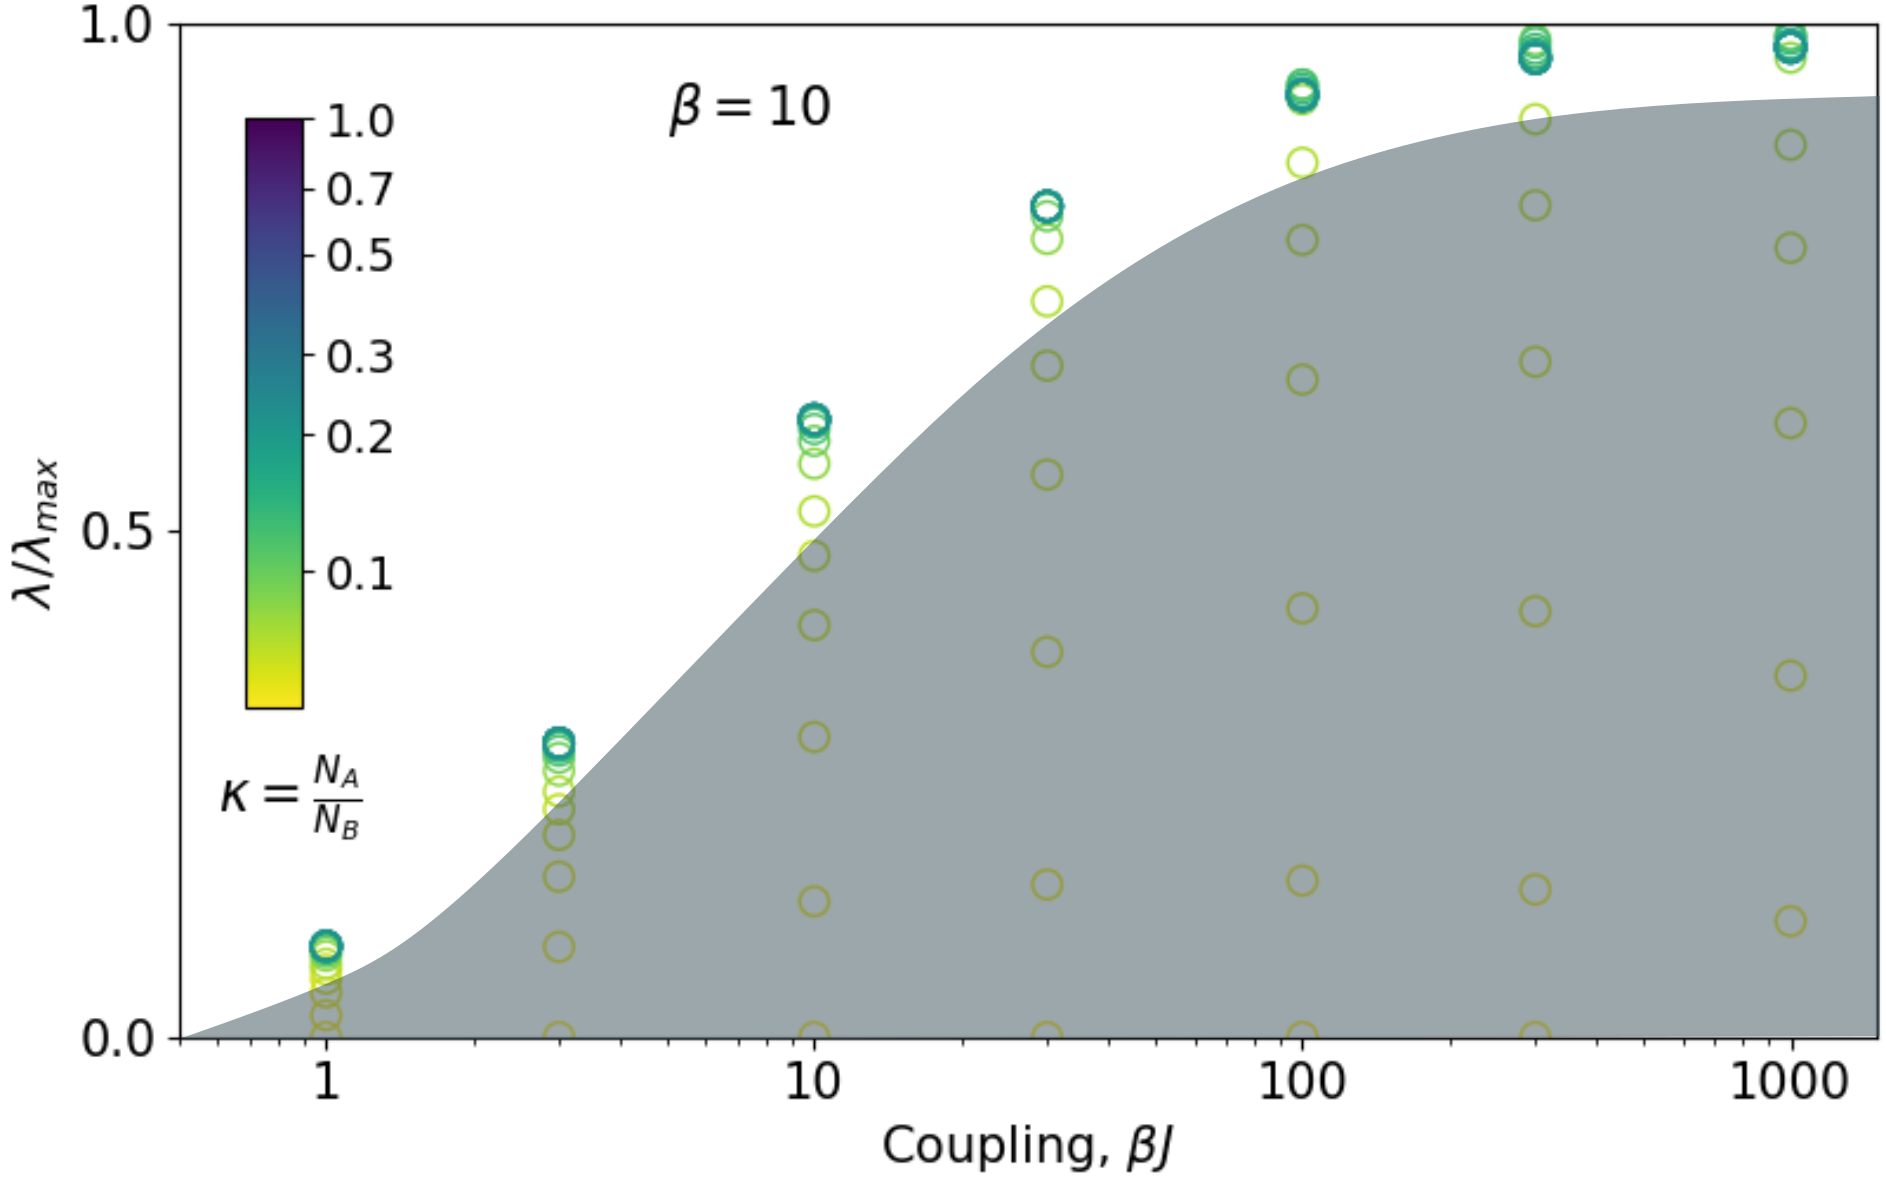
\includegraphics[width=1.00\columnwidth]{figures/chapter1/bSYK_Lyaponov_convergence.png}
	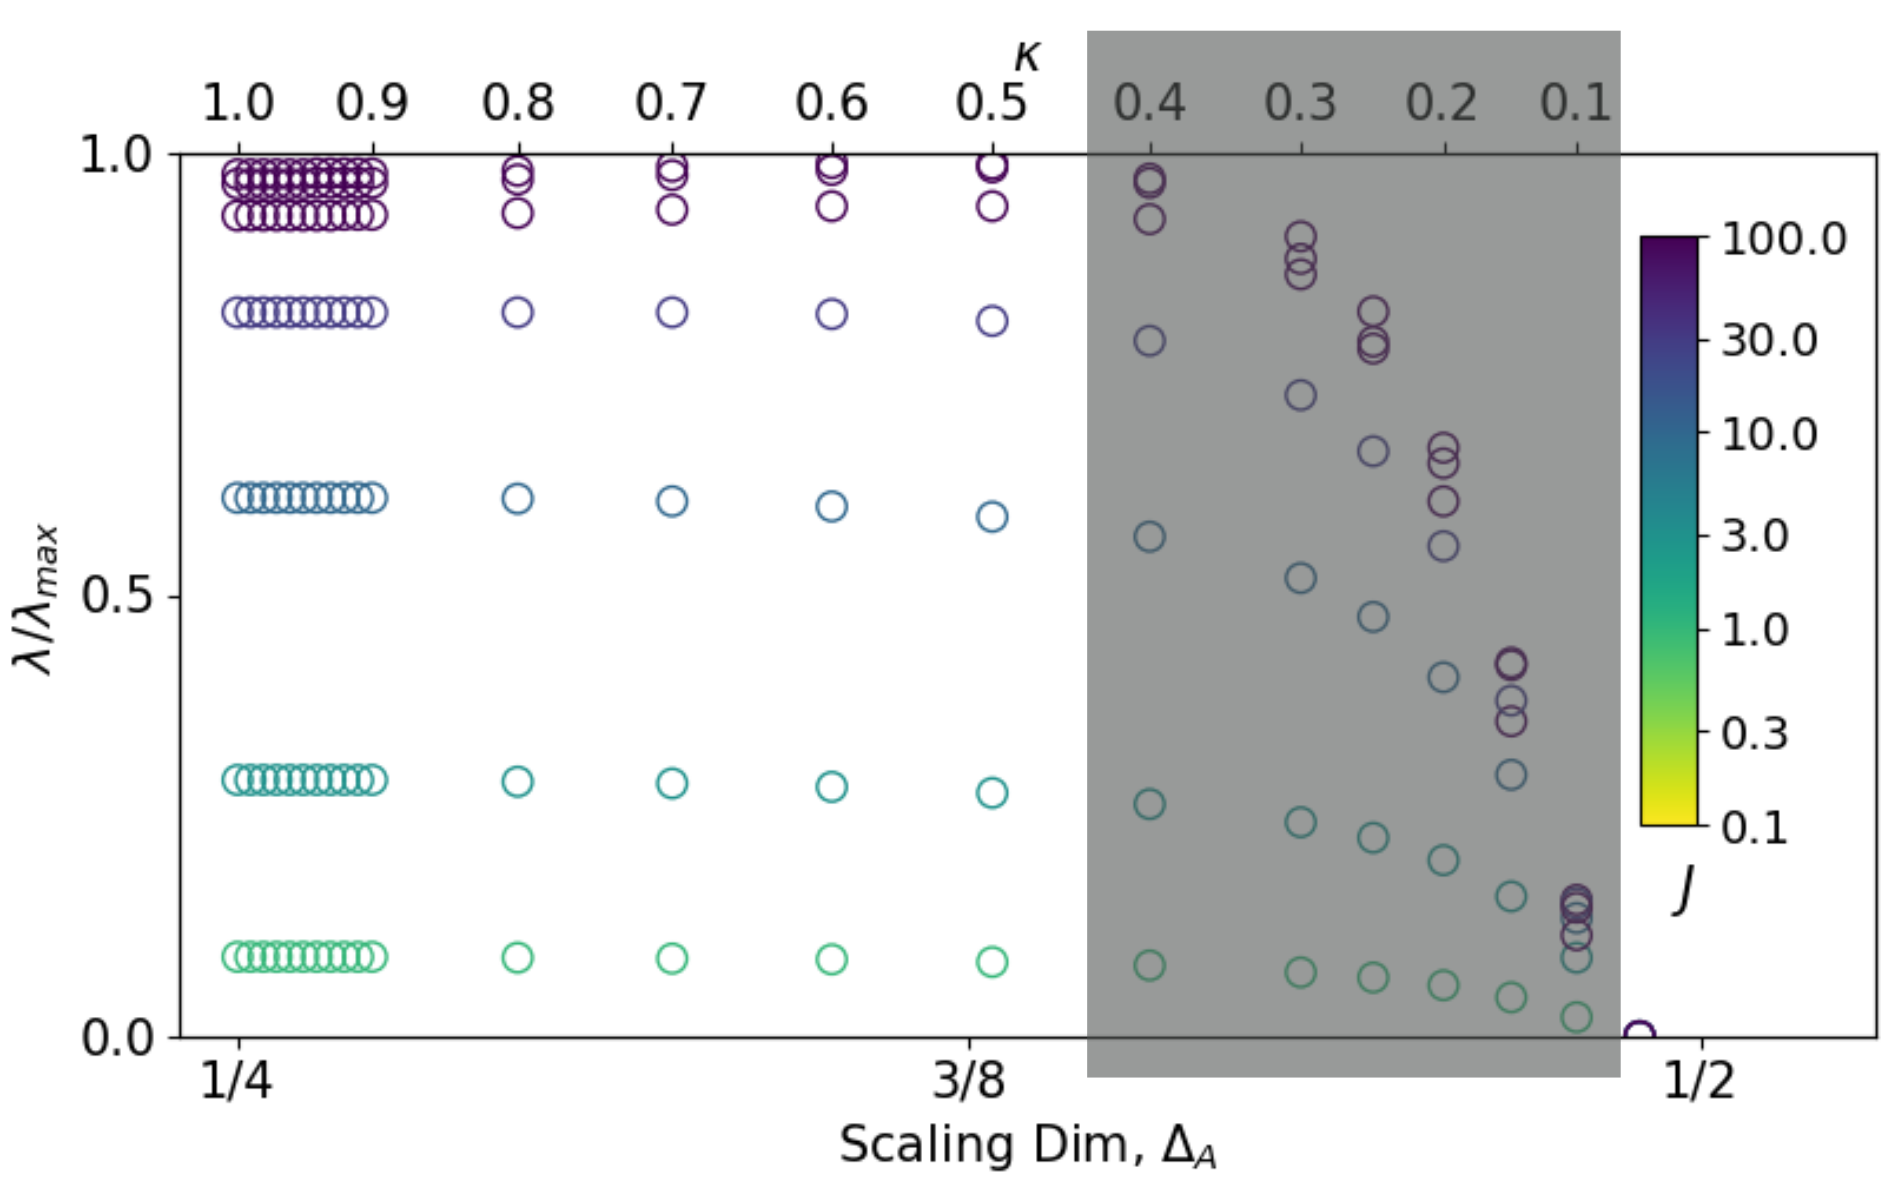
\includegraphics[width=1.00\columnwidth]{figures/chapter1/bSYK_Lyaponov_k_grid.png}
	\caption{(Left) The Lyapunov exponent as a function of the coupling strength $\beta J$ and for various values $\kappa=N_A/N_B$.
		For $\kappa > 0.7$ and $\beta J \gtrsim 300$ the b-SYK model saturates the quantum chaos bound of $\lambda = 2\pi/\beta$.
		The special case $\kappa=1$ has identical $\lambda$ as in the SYK model.
		(Right) The Lyapunov exponent as a function $\kappa$ for various values of $\beta J$.
		We find that when $\kappa \gtrsim 0.5$ then $\lambda$ is independent of $\kappa$.
		The apparent downturn of the Lyapunov exponent, as a function of $\kappa$, can be attributed to the inability of the numerics when the scaling dimensions for the two species are drastically different.
		In both figures, the grayed out region shows where the numerical results should not be trusted. 
	}
	\label{fig_Lyaponov}
\end{figure*}



\section{Results}
\label{sec_Results}
\subsection{Analytics and numerics}
We now present and discuss the results of our numerical calculations and compare to analytically known limits. This will reveal some limitations of the numerical method rooted in numerous finite size effects. 
From the analysis in the preceding chapter, we know that the Lyapunov exponent $\lambda$ is maximal in the conformal limit for all values of $\kappa$.
Furthermore, we confirmed numerically that for $\kappa=1$, then $\lambda$, as a function of $J$, has identical behavior as in the normal SYK model.
This behavior has previously been studied in Ref.~\cite{maldacena_comments_2016}. 

Numerically, we studied the behavior of $\lambda$ as a function of $\beta J$ for various values of $\kappa=N_A/N_B$.
Figure~\ref{fig_Lyaponov} (left) shows the Lyapunov exponent $\lambda$ as a function of the coupling $\beta J$ for a variety of values of $\kappa$. The different values of $\kappa$ are encoded in the color scale. We do not show values of $\kappa>1$ because they are equivalent to those for $1/\kappa$ by symmetry upon exchange of the species.
The figure suggests that $\lambda$ for all curves with $\kappa\approx1$ are approximately the same. Smaller values of $\kappa$ seem to differ significantly in their value of $\lambda$ (the gray shaded region is affected by strong finite size effects and the results should not be trusted, see discussion in Appendix~\ref{app:FiniteSize}).
We find that the numerics allows to approach the fully conformal limit of the model, meaning $\lambda/\lambda_{\rm{max}}$ approaches $1$ in the strong coupling limit for values $\kappa \approx 1$, in agreement with our analytical results.

For intermediate couplings $\beta J$, which is beyond the reach of any analytical treatment, numerical calculations are more accurate~\cite{maldacena_comments_2016}.
Similar to Ref.~\cite{maldacena_comments_2016}, we find for this regime of $J$, that the Lyapunov exponent decreases following a $1/J$ behavior.
In total, we find that for values of $0 \ll \kappa\leq 1$, the Lyapunov exponent is mostly agnostic to the population ratio $\kappa$.


It is instructive to analyze the $\kappa$ dependence in more detail.
In Figure~\ref{fig_Lyaponov} (right) we fix $J$ and vary $\kappa$ (or $\Delta_A$).
We observe that the value of $\lambda$ is \emph{independent} of $\kappa$ up to some characteristic value of $\kappa$, after which it begins to decline (grey area).
We argue that the downturn in $\lambda$ is an artifact of the numerical method we are using. Essentially we are seeing a finite-size effect in that the time/frequency discretization in the numerics is not fine enough. We have checked for isolated points that the gray area can be pushed upon increasing the resolution. 

An immediate question that follows is why the finite-size effects appear only for values of $\kappa$ away from 1. This can be understood upon considering the scaling dimensions as a function of $\kappa$: decreasing $\kappa$ increases the spread in scaling dimensions of the $A$ and $B$ Majorana fermions.
This implies that one has to keep track  of two time/and frequency scales that we need to accurately capture with our numerical frequency-grid where the scaling limit of one of the two is pushed to larger times. Getting a good resolution of that requires a finer frequency grid at small frequencies.
When $\kappa$ deviates too much from 1 this becomes increasingly costly in terms of time/frequency steps. An extended discussion of the finite size effects in the two-fermion Green function is given in Appendix~\ref{app:FiniteSize}.


\subsection{Discussion and Conclusion}


Having established that the Lyapunov exponent is independent of $\kappa$, 
we can compare our results to a similar model presented in Ref.~\cite{chen2017tunable}.
In that case, the authors find a Lyapunov exponent in the conformal limit which can be tuned by adjusting the relative populations of the different species of fermions. In our model, we find a stark contrast to this behavior.
Instead, we find that our model's Lyapunov exponent is completely impervious to the relative number of fermion species. In the conformal limit,
aside from showing this result in an explicit analytical calculation,
we can motivate the result in a physical way, as a sort of "proof by contradiction".
If for example, the $A- $ flavor Majorana had a smaller Lyapunov exponent,
the diagrams contributing to its four point function proceed by a pathway in which they scatter into two $B- $ flavor Majoranas,
which would then propagate with the greater Lyapunov exponent,
before finally scattering back into two $A- $ flavor Majoranas. This forces both flavors to have exactly the same exponent,
and a mathematical version of this argument is presented in Appendix~\ref{sec:technical_explanation}.  


The two-point function of the Majoranas are characterized by their scaling dimension,
which is quite sensitive to the relative population ratio $\kappa$,
so one would expect that the four-point function as characterized by the Lyapunov exponent would depend on $\kappa$ as well,
but we have shown conclusively that this is not the case for cases of strong, intermediate and weak coupling, which is quite surprising.
An interesting future direction of study would be to consider what deformations should be introduced to the theory in order to have a different Lyapunov exponent for the two flavors of Majoranas.

The present work on the calculation of the Lyapunov exponent in the b-SYK model shows that the features of emergent conformal symmetry and maximal quantum chaos of the SYK model are quite robust to the couplings obeying additional internal symmetries.
Besides the particular model considered here, there are many setups where parity, charge, spin,
or general flavor symmetries of the underlying fermions carry over to the interaction matrix elements~\cite{Chowdhury-RMP2022,Franz2018-review,Kim2019,sahoo_traversable_2020,xu_sparse_2020}.
The methods used here readily carry over to those models and can be applied to the calculation of Lyapunov exponents and, in general, to the analysis of Bethe-Salpeter equations.


\section*{acknowledgments}
	We acknowledge discussions with Y. Cheipesh, A. Kamenev, K. Schalm, M. Haque, and S. Sachdev. Extensive discussions with D. Stanford about the conformal limit of the OTOC are also acknowledged.
	SP thanks E. Lantagne-Hurtubise, O. Can, S. Sahoo, and M. Franz for many useful discussions related to SYK models and holography.  This work is part of the D-ITP consortium,
	a program of the Netherlands Organisation for Scientific Research (NWO) that is funded by the Dutch Ministry of Education, Culture and Science (OCW).
	SP received funding through the European Research Council (ERC) under the European Union's Horizon 2020 research and innovation program.


\section*{Author Contributions}
A.S.S and M.F contributed equally to this work.

% \appendix
\newpage
\section{Appendix}

\subsection{Mathematical consistency of the Lyapunov ansatz}
\label{sec:technical_explanation}

The following short consideration for the diagram piece $\mathcal{F}_{00}$ shows why we expect only one `global' Lyapunov exponent for all scattering channels.
The other components of the four-point function can be treated with exactly the same argument. The starting point is
%
\begin{multline}
	\mathcal{F}_{00}(t_1,t_2) = \int dt_3 dt_4\, K_{00}(t_1,t_2,t_3,t_4)\mathcal{F}_{00}(t_3,t_4) \\ + K_{10}(t_1,t_2,t_3,t_4)\mathcal{F}_{10}(t_3,t_4)
\end{multline}
%
where we use the definition 
%
\begin{align}
	t_{1,2} &= t \pm \frac{1}{2}t_{12} \nonumber \\
	t_{3,4} &= \tilde{t} \pm \frac{1}{2}t_{34} \;.
\end{align}
%
The factors of a half were included to keep the area element invariant under this transformation,
$dt_3dt_4 = d\tilde{t}dt_{34}$. After some algebra, for the ansatz $f_{00}$ one finds
%
	\begin{multline}
		f_{00}(t_{12}) = 
		J^2\frac12 \left(1+ \frac1\kappa\right) \int d\tilde{t}dt_{34} G^R_A(t_{13})G^R_A(t_{24})\Big{[}\frac{1}{\kappa}\left(G^W_B(t_{34})\right)^2 e^{\lambda_{00}\tilde{t} - \lambda_{00} t}f_{00}(t_{34}) + \\  \left(G^W_A(t_{34})G^W_B(t_{34})\right) e^{\lambda_{10}\tilde{t} - \lambda_{00} t}f_{10}(t_{34}) \Big{]}
	\end{multline}
%
Now we Fourier transform according to 
%
\begin{equation}
	G^W_A(t_{34}) = \int \frac{\dd\omega_a}{2\pi} e^{-\i\omega_a t_{34}} G^W_A(\omega_a)\;.
\end{equation}
	If we calculate a sample term $f_{00}$ to illustrate the point, 
	\begin{multline}
		f_{00}(\omega) = J^2\frac12 \left(1+ \frac1\kappa\right)\int \dd t_{12} e^{\i\omega t_{12}}\int \dd \tilde{t}\int \dd t_{34} \int \frac{\dd\omega_a}{2\pi} e^{-\i\omega_a(t - \tilde{t} + \frac{1}{2}(t_{12}-t_{34}))}\int \frac{\dd\omega_b}{2\pi} e^{-\i\omega_b(t - \tilde{t} - \frac{1}{2}(t_{12}-t_{34}))} \\
		G^R_A(\omega_a)G^R_A(\omega_b)\int\frac{\dd\omega_c}{2\pi}\int\frac{\dd\omega^\prime}{2\pi} e^{-\i(\omega_c +\omega^\prime)t_{34}}
		\left[\tilde{K}_{00}(\omega_c)f_{00}(\omega^\prime) e^{\lambda_{00}\tilde{t} - \lambda_{00}t} + \tilde{K}_{10}(\omega_c)f_{10}(\omega^\prime) e^{\lambda_{10}\tilde{t} - \lambda_{00}t}\right]
	\end{multline}
we notice that there are three time integrations that result in delta functions,
but 4 $t$-like variables. In the case of the first term in the square brackets,
since it only appears in the combination $(\tilde{t} - t)$, this eliminates a variable,
and there are sufficient constraints to make it only depend on $\omega$ variables. However,
in the new term coming from flavor-mixing of the b-SYK, this is not true any more.
This is a signal of a breakdown of the ansatz Eq.~\eqref{eq:Lyapunov_Ansatz}.
We thus see that for consistency we must impose that $\lambda_{00} = \lambda_{10}$.
By repeating the argument for the other components of $\mathcal{F}$,
it can be shown that all Lyapunov components should be the same, $\lambda_{ij} = \lambda$,
and that there is only one Lyapunov exponent governing the behavior of the model.

\subsection{Recovery of the maximal Lyapunov exponent of the regular SYK}
At $\kappa=1$, the numerics reflect that the Lyapunov exponent of the model is the same as the maximal value of regular SYK. This can be understood by looking at the kernel Eq.~\eqref{eq:kernel_tau}. At $\kappa=1$, the scaling dimensions of both the $A$ and $B$ majoranas become $\frac{1}{4}$, and hence $G^A(\tau) = G^B(\tau) \equiv G(\tau)$, the 2 point function of regular SYK. The kernel then factorizes into the product of a function of the four imaginary times, and a constant matrix. 
\begin{equation}
	K(\tau_1\cdots\tau_4) = -J^2 G(\tau_{13})G(\tau_{24})G(\tau_{34})^2 \begin{pmatrix}
		1 & 2 \\
		2 & 1
	\end{pmatrix}
\end{equation}
The constant matrix in question has eigenvalues $-1$ and $+3$. The latter eigenvalue makes the kernel mathematically the same as the one for regular SYK, and hence the Lyapunov exponent should be the same.  Furthermore, it is for this reason that the special case of $\kappa=1$ allows the kernel to be diagonalized in the basis of the conformal blocks labeled by $h$. For $\kappa \neq 1$, the four components of the kernel transform differently under transformations of the conformal group. 



\begin{figure}[h]
	\centering
	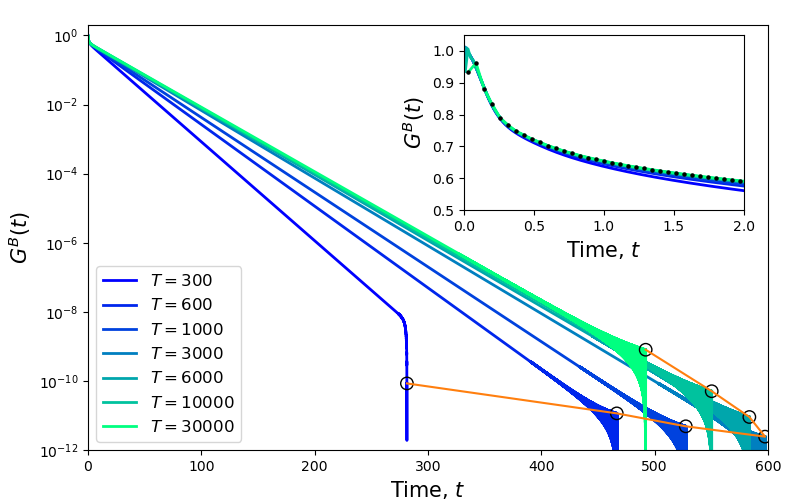
\includegraphics[width=1.0\columnwidth]{figures/chapter1/FiniteSizeAnalysis.png}
	\caption{The Green function $G^B(t)$ for $\kappa=0.3$, $\beta=10$, $J=10$. 
		The number of discretization points is fixed to $N=2^{19}$ and the length of the time-grid $T$ is varied.
		The figure shows that increasing $T$ gives a better estimate of the decay-time for the Green function, but if $T$ is taken to be too high, numerical accuracy of the Green function is lost. The sweet-spot is here at $T=3000$.
		Black circles marks the position of (the point before) the first negative $G$, and is an estimate of the size of the numerical noise.     
	}
	\label{fig:FiniteSize}
\end{figure}



\subsection{Finite-size dependence of two-point functions and Lyapunov exponents}\label{app:FiniteSize}
In this section, we briefly comment on the sensitivity of the two-point function to the finite-size cut-offs introduced when numerically solving the Schwinger-Dyson equations for the b-SYK model.
To solve the coupled b-SYK equations (Eq.~\eqref{eq:retarded_dyson_equation} and below), we discretize the semi-infinite positive timeline by introducing a long time cut-off $T$ and a finite number of time steps $N$ inbetween. 
This introduces a discretized time-step $\Delta t=T/N$ and frequency step $\Delta \omega = 2 \pi / T$.
To avoid the discontinuities at $\omega=0$ and $t = 0$, we choose a time grid that is $t_n = \Delta t \cdot (n+1/2)$, and similarly for the frequency grid.

We can study of the effects of varying $T$ and $N$ on $G^B(t)$.

In Figure~\ref{fig:FiniteSize} we show an example for $\kappa=0.3$, $\beta=10$, and $J=10$.
We fix the number of discretization points to $N=2^{19}$ and plot $G^{B}(t)$ for several values of $T$. We have cut off the plot at the first negative value of $G^B$.
In the plot, we observe two qualitative effects of changing $T$: First, upon increasing $T$,
we find that the decay time (slope) of the Green function increases (decreases). Thus, increasing $T$, we allow $G^B(t)$ to behave as if the time axis was really semi-infinite.
One can perform a $1/T$ analysis and finds that the lines have a well-defined slope in the $T\to\infty$ limit.

Secondly, which is more subtle, we see that making $T$ too large decreases the quality of the approximation for $G^B(t)$, with the optimal number being around $T=3000$.
We arrive at this number by the following argument: In the plot, we only show $G^B(t)$ until the first non-negative value (at time $t_C$).
The solid-looking wedge shape that appears just before the first negative number is the effect of numerical oscillations that (as $G$ decreases) become relatively more important.
From the height where the ``wedges'' disappear (black circles connected with an orange line), we can approximate the size of this numerical error.
By inspection, we see that the smallest numerical errors (and also the largest $t_C$) happen for $T=3000$.
We can understand the loss by noting that as $T$ grows, then (for fixed $N$) $\Delta t$ also grows.
In the inset of the figure, one can see that at $T=30000$, $\Delta t$ is so large that it even affects the continuity of the curve $G^B(t)$.

Choosing the appropriate $T$, is thus affected by the range of the Green function decay, which in turn is affected by $\kappa$, the ratio between the two species.
In the numerics that we present in the main text, we worked with a fixed $N$ and $T$, which are good when $\kappa\approx1$ but not when $\kappa$ is increasingly asymmetric.
Errors in the two-point function will propagate and influence the calculations of the Lyapunov exponent and explain why we see the downturn of $\lambda$ at a characteristic value of $\kappa$.



		% \chapter{Dense Entanglement in Critical States}
\label{ch:EE}

\section*{Abstract}
	At critical points the entanglement between microscopic degrees of freedom is thought to be maximal, and proportional to the number of dynamical fields. In 1D systems this is analytically known and numerically verified through the knowledge that the bond dimension in tensor network states represents the upper bound on the amount of entanglement a system can represent. Here we test this in 2D systems using Carleo \& Troyer neural-network quantum states in solving many-body quantum systems at their criticality. We postulate that for a neural-network quantum state (NQS) at criticality the entanglement is bounded by the ratio of the number of visible ($N$) and hidden nodes ($M$), $\alpha = M / N$. Computing the entanglement as a function of $\alpha$ at criticality in $Z_2^n/Z_2$ lattice gauge theories, allows us to study entanglement at criticality for differing number of dynamical fields. Surprisingly we do not find a linear relation.
	
\section{Introduction}

Though the idea precedes it by a number of years, the notion to use entanglement to classify the ground states of quantum many body systems really took off with the discovery of the topological insulator. Ordinary states of matter with quasi-particle expectations around a trivial IR fixed point are short range entangled states. Topological insulators with a gap that separates the bulk spectrum from the topological (edge) modes are long range   sparsely entangled states. Sparse, because the number of topological modes is very small compared to the exponentially  large number of  excitable modes in the full Hilbert space. It also raises the immediate question whether there are long range {\em densely} entangled states of matter. Such states are arguably the most quantum many-body state possible and have been coined quantum supreme matter.

Frustrated systems and quantum spin liquids are possible candidates. But another possible candidate is a theory right at the non-trivial IR fixed point of a second order phase transition where the correlation length is infinite. As no length scale remains, there cannot be either short or long range entanglement. Entanglement must exist at all scales.\footnote{The remarkable connections between quantum entanglement and emergent geometry in holographic theories suggest that the non-trivial IR fixed point dual to extremal black holes are of this type \cite{zaanenHolographicDualityCondensed2015,hartnollHolographicQuantumMatter2018}.} This is exemplified by the classic calculation of the entanglement entropy in 1+1D conformal field theories \cite{Holzhey:1994we}
\begin{equation}
	\label{eq:1DCFT-EE}
	S_{\text{1D CFT}} = \frac{c}{3}\ln(\ell/a) \mathperiod
\end{equation}
Here $\ell$ is the size of the region (the area) for which the entanglement with the complement is computed; $a$ is a UV cut-off, and $c$ is the central charge of the theory. Since the central charge is a measure of the number of degrees of freedom in the system, the scaling of the entanglement entropy with $c$ shows that all degrees are involved and entanglement is both dense and long range.

An illustrative example of the dense entanglement in critical states is from a study of such 1D systems using the Multi-Scale Entanglement Renormalization Ansatz (MERA) \cite{Evenbly2013}. Similar to Matrix Product States (MPS), these are variational descriptions of many-body-ground states designed to track (up to area-scaling) entanglement in terms of the bond-dimension of the variational state. MERA improves on MPS by engineering in critical behavior from the start. Tuning such a 1D MERA system to criticality one indeed sees that to ensure the same accuracy in the ground state energy, the minimal bond dimension must grow exponentially with the central charge. Since the bond dimension is designed to scale as $D \sim \exp(S_{\text{1D CFT}})$, this includes the scaling with the central charge, consistent with Eq.(\ref{eq:1DCFT-EE}).

The aim of this paper is to verify that this similar exponential increase in entanglement at critical states also happens in 2D systems. An extension of MERA to 2D systems is notoriously difficult. However, the advent of neural network machine learning techniques, has given us an inroad to this question. From Neural Quantum States \cite{doi:10.1126/science.aag2302, Vicentini:2021pcv}, where the many-body groundstate is contructed as a variational wavefunction based on a Restricted Boltzmann Machine neural network, one can also get an estimate of the entanglement or rather the entanglement entropy between two spatially separated parts of the groundstate wavefunction \cite{Shi_2019}. The power of this approach is that it is not limited to 1D systems \cite{Vicentini:2021pcv}. It works in principle in any dimension and is only limited by computational time. 

The question that remains then is which 2D systems to use. Though one can simply study the approach to a critical point, one would need a notion of a central charge to make a fully equivalent statement compared to 1D systems. Of course there is no notion of a central charge in 2D systems. However, using that the central charge encodes for the number of degrees of freedom, we can rely on a recent finding that there is a nice sequence of critical points in classical 3D $Z_2\times Z_2 \times \ldots \times Z_2/Z_2$ gauge theory \cite{Bukva:Registry}.\footnote{This is inspired by orbifold models of 1D systems.} With each additional $Z_2$ matter factor the number of degrees of freedom increases, yet in all other aspects the critical points are similar. The thermodynamics of these classical 3D systems corresponds to the quantum groundstate of 2D gauged transverse field Ising models \cite{transferMatrix1978,fradkinPhaseDiagramsLattice1979,RevModPhys.51.659}. It is then natural to suppose that one finds an increase in the entanglement in the groundstates of 2D $Z_2$ gauged transverse field $Z_2\times Z_2 \times \ldots \times Z_2$ Ising at criticality proportional to the number of matter fields involved. That all matter fields are involved is suggested by the nature of the phase transition: it belongs to the $p=2^{N_{\text{rep}}-1}$-Potts universality class \cite{Bukva:Registry}.

In section \ref{sec:lat-gauge} we set up the RBM based Neural Quantum State variational approximation to the groundstate wavefunction of $(Z_2)^n/Z_2$ gauged transverse field Ising. Computationally we will limit our attention to $n=2,3,4$. We then compute the Entanglement Entropy between two parts of the system in section \ref{sec:ee}. The results are partially surprising. We see the rise in entanglement entropy as we approach the critical point corresponding with the absence of a scale and hence densification of entanglement. However, at criticality we do not see the expected increase in the entanglement entropy corresponding to the increase in the number of matter fields. In fact the entropy exhibits a puzzling behavior with increasing matter fields.
We discuss possible explanations for this unexpected finding in the conclusion section \ref{sec:conclusion}.

\section{Neural Quantum State approximation to groundstates of $Z_2\times Z_2 \times \ldots \times Z_2/Z_2$ transverse field "Ising" lattice gauge theory}
\label{sec:lat-gauge}

\subsection{NQS from RBM Set-Up: application to $Z_2$ gauge theory}
A Neural Quantum State (NQS) is a variational wave function ansatz based on a Restricted Boltzmann Machine (RBM). It
was introduced by Carleo \& Troyer \cite{doi:10.1126/science.aag2302} inspired by the use of RBMs in machine learning problem but now applied to minimize the ground state of a given Hamiltonian. Consider a system with $N$ spin-1/2 spins labeled as $S = (s_1, s_2, \dots, s_N)$ with $s_i \in \{-1,1\}$. Then the RBM represents a wave function in the following way: The physical spins are complemented by hidden spins $H= (h_1,\dots,h_M)$ with $h_i = \{-1,1\}$ . Then one posits the variational function for the quantum state:
\begin{equation}
	\Psi_M(S,\mathcal{W}) = \sum_{h_i} e^{\sum_j a_j s_j + \sum_i b_i h_i + \sum_{ij} W_{ij}h_i\sigma_j^z} \mathcomma
\end{equation}
which depends on the values of the weights as $\mathcal{W}=(a_i, b_j, W_{ij})$. These weights form 
a network (Fig.\ref{fig:rbm}) and the expression resembles a Boltzmann sum over the $h_i$ configurations.
\begin{figure}[H]
	\centering
	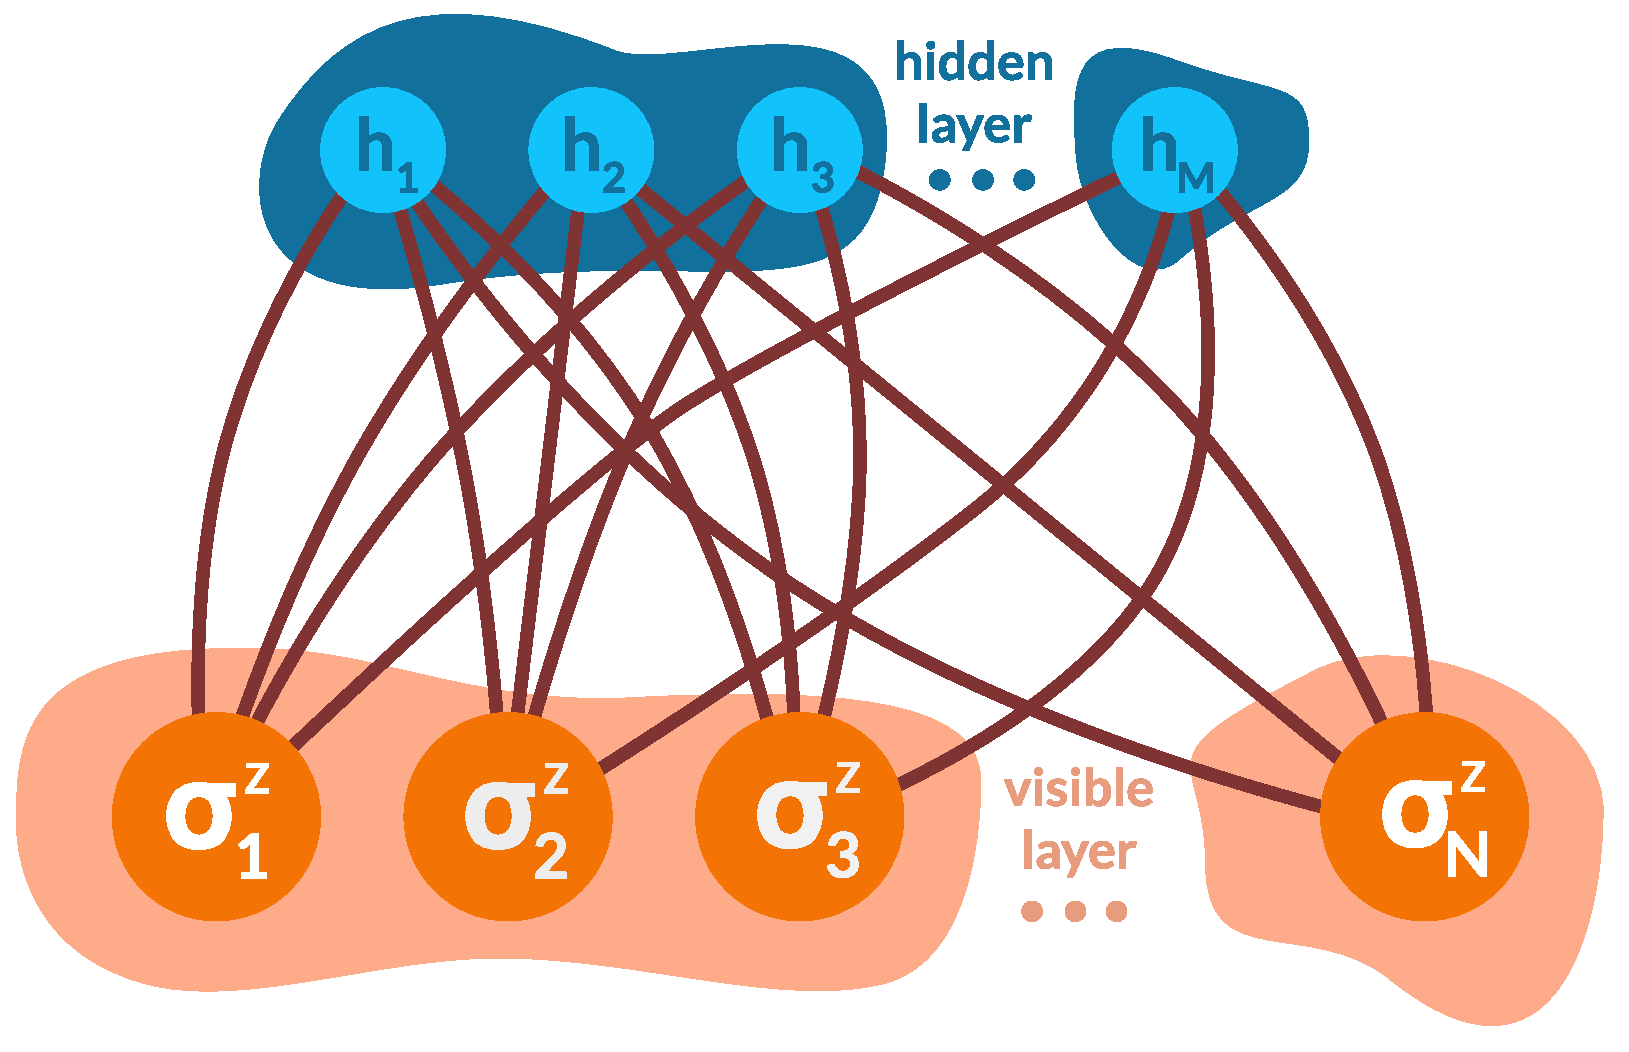
\includegraphics[width=0.5\textwidth]{figures/chapter3/rbm.pdf}
	\caption{Illustration of a restricted Boltzman machine (RBM) neural network.}
	\label{fig:rbm}
\end{figure}
\noindent
The qualification Restricted refers to the fact that the weights (interactions) only connect visible and hidden spins, and there are no weights amongst hidden spins. Because of this lack of inter-hidden layer connectivity of an RBM  all hidden variables can be traced out which leaves us with:
\begin{equation}
	\Psi(S,\mathcal{W}) = e^{\sum_i a_i s_i} \prod_{i=1}^{M} 2 \cosh(b_i + \sum_j W_{ij}s_j) \mathcomma
\end{equation}    
Following the algorithm from \cite{doi:10.1126/science.aag2302} we can train this network to efficiently represent the ground state of our Hamiltonian.


The reason we choose a NQS variational method is that one can readily compute the entanglement entropy in the (approximate) groundstate.
To exhibit dense entanglement at criticality in 2D systems, we wish to compute the entanglement entropy on a set of related theories that has tuneable set of degrees of freedom. A family of such theories are $Z_2\times Z_2 \ldots Z_2/Z_2$ multiple Ising matter fields gauged with $\mathbb{Z}_2$ symmetry on a 2+1D lattice \cite{Bukva:Registry}. These are extensions of the well known $Z_2/Z_2$ lattice gauge theory with Higgs fields from Fradkin and Shenker \cite{fradkinPhaseDiagramsLattice1979}. On the sites of a lattice, labeled by $\vec{r}$, we have $n$-Ising matter fields ($\sigma^i(\vec{r})$, $i=1\ldots n$) and on the links in the direction of the lattice vector $\hat{e}_\mu$ we have an Ising gauge field ($U(\vec{r},\hat{e}_{\mu})$. The action of a $d+1$ dimensional model on a hypercubic lattice is defined as:
	\begin{equation}
		\begin{split}
			&S(\sigma(\vec{r}), U(\vec{r},\hat{e}_{\mu})) =
			J \sum_{i=1}^n\sum_{\vec{r}, \mu} \sigma^i(\vec{r}) U(\vec{r},\hat{e}_{\mu}) \sigma^i(\vec{r} + \hat{e}_\mu)  \\ &+ K \sum_{\vec{r}, \mu \nu} 
			U(\vec{r},\hat{e}_{\mu}) U(\vec{r} + \hat{e}_\mu,\hat{e}_{\nu}) U(\vec{r}+\hat{e}_{\nu}+\hat{e}_{\mu},-\hat{e}_{\mu}) U(\vec{r}+\hat{e}_{\nu},-\hat{e}_{\nu}) \mathperiod
		\end{split}
	\end{equation}
	This action is invariant under the local $\mathbb{Z}_2$ gauge transformations:
	\begin{equation}
		\begin{split}
			\sigma^i(\vec{r}) &\rightarrow 
			= \sigma^i(\vec{r}) s(\vec{r}) \mathcomma \\
			U(\vec{r},\hat{e}_{\mu}) &\rightarrow s(\vec{r})U_\mu(\vec{r},\hat{e}_{\mu})s(\vec{r} + \hat{e}_\mu) \mathcomma
		\end{split}		
	\end{equation}
	where $s(\vec{r}) = \pm 1$. Though for $n=1$ there is famously no phase transition at $K=0$ as a function of $J$ illustrating the formal equivalence between the confining ($J<0$) and Higgs ($J>0$) phase of the $Z_2/Z_2$ theory, for any $n \geq 2$ there is a second order phase transition at finite $J$ between an disordered $J<0$ and ordered phase $J>0$ \cite{Bukva:Registry}. The phase transition belongs to the $p=2^{n-1}$-Potts universality class and is characterized by an expectation value of the (gauge invariant) registry order parameters $\langle \sigma^1\sigma^2\rangle$,  $\langle \sigma^1\sigma^3\rangle$, \ldots, $\langle \sigma^{n-1}\sigma^n\rangle$. We will use the product of all order parameters to measure all of them simulataneously $\langle \sigma_1^{n-1}\sigma_{2}^{n-1}\ldots \sigma_n^{n-1}\rangle =\prod_{i<j}\langle \sigma_i\sigma_j\rangle +\ldots $. This implies that the 2D quantum system corresponding to this system has a quantum phase transition with critical behavior at the corresponding point. The corresponding quantum Hamiltonian can be derived using transfer matrix formalism. Following \cite{transferMatrix1978,RevModPhys.51.659} we find a $Z_2$ gauged transverse field Ising Hamiltonian 
	\begin{align}
		\label{eq:gaugeHamiltonian} 
		H = &-\sum_{i, \vec{r}} \sigma_1^i(\vec{r}) - \sum_{\vec{r}, \mu} \tau_1(\vec{r},\hat{e}_{\mu})
		-\lambda \sum_i\sum_{\vec{r}, \mu} \sigma_3^i(\vec{r})\tau_3^\mu(\vec{r})\sigma_3^i(\vec{r}+\hat{e}_\mu) 
		\\ & 
		-\omega \sum_{\vec{r}, \mu \nu} \tau_3(\vec{r},\hat{e}_{\mu})\tau_3(\vec{r}+\hat{e}_\mu,\hat{e}_{\nu})\tau_3(\vec{r}+\hat{e}_\nu,\hat{e}_{\mu})\tau_3(\vec{r},\hat{e}_{\nu}) \mathcomma \nonumber
	\end{align}
	where now the matter fields $\sigma^i$ and the gauge field $\tau$ are Pauli matrices acting on sites and links of a 2D lattice, and we used that for a $Z_2$ symmetry the link is its own Hermitian conjugate $\tau(\vec{r}+\hat{e}_{\mu},-\hat{e}_{\mu})=\tau(\hat{r},\hat{e}_{\mu})$. The coupling coefficients $\lambda$ and $\omega$ can be related to $K$ and $J$ in the 2+1D classical action formulation, but the precise relation is unimportant. We shall set $\omega =0$ and keep $\lambda$ undetermined.  
	What is important for our NQS variational approach is that 
	physical states of this theory must satisfy the gauge invariance constraint. So therefore must the NQS itself. The local gauge transformations are generated by $G(\vec{r})=\prod_i\sigma_1^i(\vec{r})\prod_{\mu}\tau_1(\vec{r},\hat{e}_{\mu})$ at each site $\vec{r}$. Every physical state $\ket{\psi}$ must therefore obey
	\begin{equation}
		G(\vec{r}) \ket{\psi} = \ket{\psi}
	\end{equation}
	for every site $\vec{r}$ of the lattice. This constraint can easily be visualized in the $\tau_1$ and $\sigma_1$ basis Fig.\ref{fig:contraint}, basically every site needs to have $n+m =2 k, k\in\mathbb{Z}$ with $n$ the number of down spins on and $m$ the number of down-links emanating from the site. 
	
	\begin{figure}[H]
		\centering
		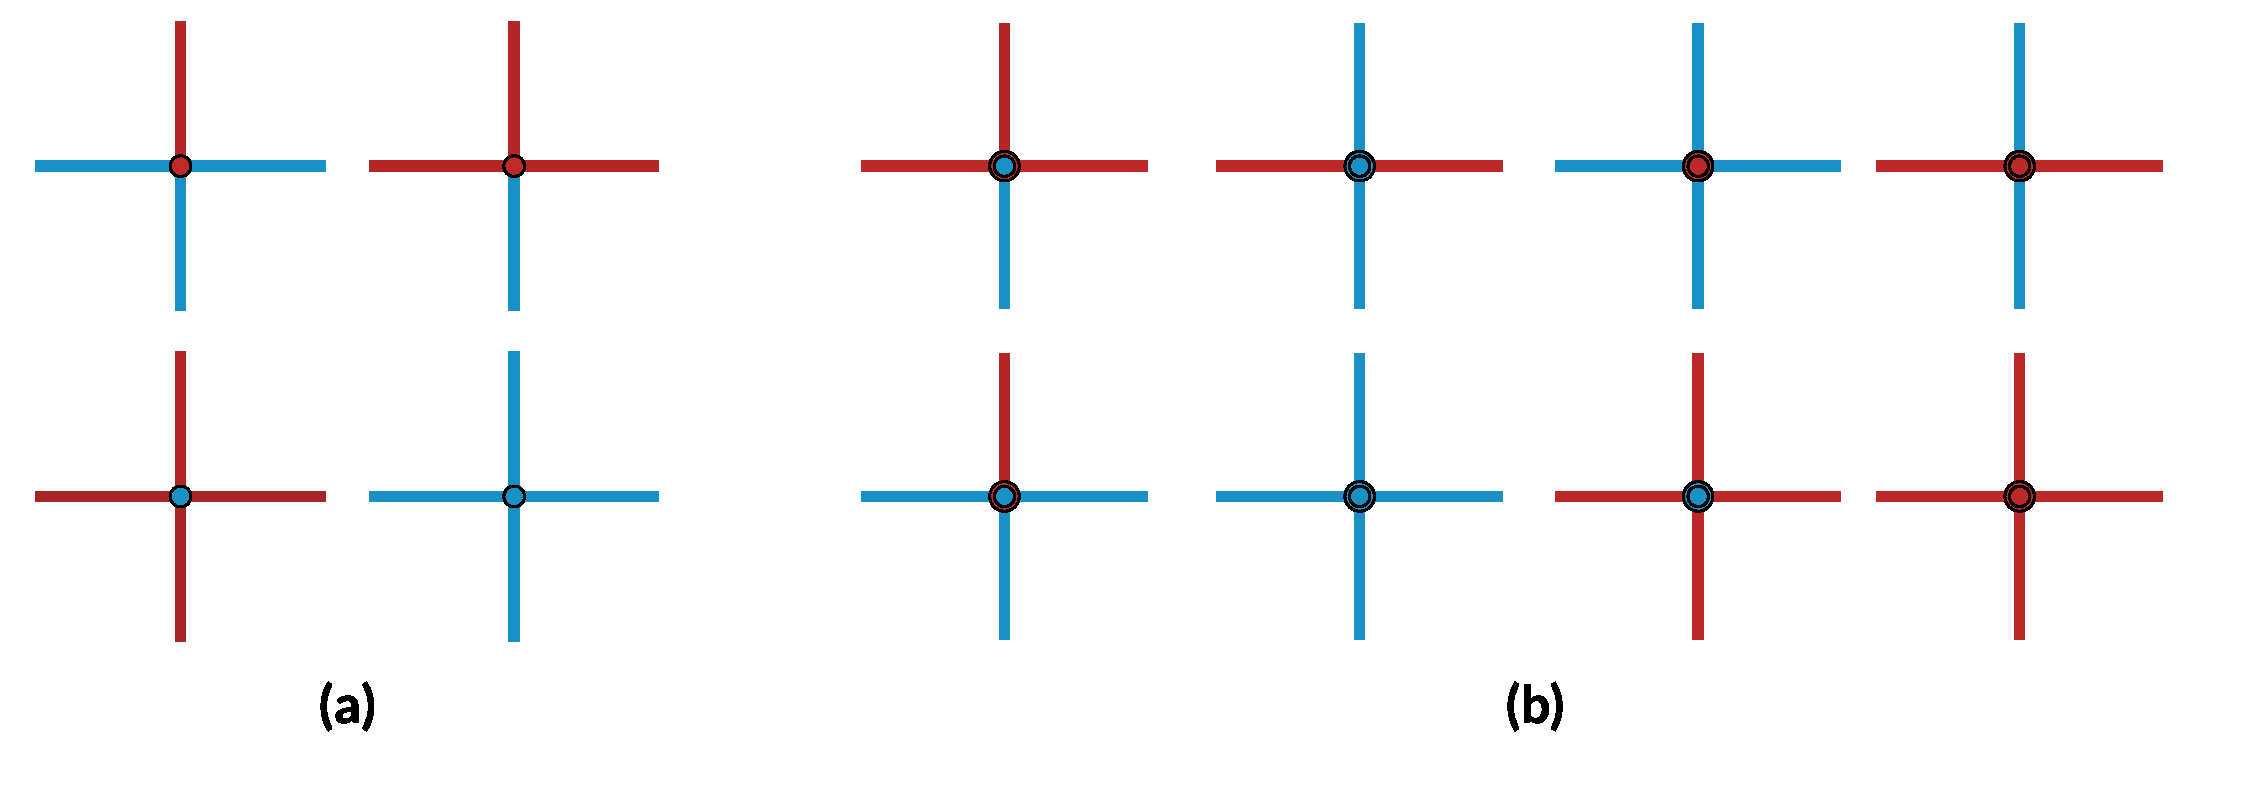
\includegraphics[width=0.65\textwidth]{figures/chapter3/constraint.pdf}
		\caption{Visualization of the gauge constraint in $\tau_1$ and $\sigma_1$ basis. \textcolor{myred}{Red} color represents down spins (-1) and \textcolor{myblue}{blue} up spins (+1). \textbf{(a)} Different gauge invariant combinations in the case of $Z_2 / Z_2$ theory. \textbf{(b)} Different gauge invariant configurations for the $Z_2 \cross Z_2 / Z_2$ theory. For the visual purposes spins at the nodes of a lattice for two fields are different sizes, so they can be distinguished in the diagram.}
		\label{fig:contraint}
	\end{figure}
	
	The NQS wavefunction itself is approximated by MCMC sampling. Due to the gauge constraint, this has to be done with care, because the naive Hilbert space is now larger than the space of physical states. We employ a simple updating procedure that always flips two matter spins, a matter spin and a link, or two links on a site to remain within the physical Hilbert space. For alternate approaches to NQS states for gauged lattice models, see \cite{luoGaugeEquivariantNeural2021}. 
	
	\section{Entanglement entropy}
	\label{sec:ee}
	
	The reason we resort to NQS to approximate the ground state is that entanglement or rather the entanglement entropy can be readily computed for such wavefunctions. Entanglement entropy is of course only a partial measure of entanglement, but to first approximation it should be able to quantify its denseness. Given a system described by a density matrix $\rho$ and divided into two parts, $A$ and $B$, then the entanglement entropy between these parts is defined as:
	\begin{equation}
		\label{eq:EE}
		S_A = -\tr \left[\rho_A \log \rho_A\right] ~,~~~~\rho_A =\text{Tr}_B\rho~.
	\end{equation}
	If the original state is pure, as is the case here, then $S_B=S_A$.\footnote{
		An important comment is that one has to be careful in computing the entanglement entropy in gauged theories, see e.g. \cite{Trivedi}. As our algorithm specifically only limits to physical states, this is not an issue, and we can use the standard expression Eq.(\eqref{eq:EE}).}
	
	Quite generally, for a system decomposable into two parts $A$ and $B$, the (ground)state can be written as
	\begin{equation}
		\ket{\Psi} = \sum_{i,j} c_{i,j} \ket{i}_A \otimes \ket{j}_B~.
		\label{eq:stateDecomp}
	\end{equation}
	The coefficients of the expansion $c_{i,j}$ can be combined in one probability-amplitude matrix where each element at the coordinates $i$,$j$ would be a probability-amplitude that we find the system with part $A$ being in the state $i$ and part $B$ being in the state $j$. 
	The entanglement entropy can be computed
	using Schmidt/Singular Value Decomposition (SVD); see \cite{Shi_2019} in the context of NQS or e.g. \cite{2011arXiv1109.0104M} in the contect of MCMC. We write the probability-amplitude matrix as:
	\begin{equation}
		c_{i,j} = U_{i,k}\Sigma_{k,l}V^\dagger_{l,j}~.
	\end{equation}
	If we label with $N_A$ and $N_B$ the sizes of parts $A$ and $B$ respectively, then $U, \Sigma$ and $V^\dagger$ are matrices of dimensions $N_A \cross N_A$, $N_A \cross N_B$ and $N_B \cross N_B$, where $\Sigma_{kl}=\sigma_k\delta_{kl}$ is a ``diagonal'' matrix with singular (i.e. non-negative real) values on the main diagonal and zeros otherwise. 
	Using this decomposition the entanglement entropy is easily seen to equal
	\begin{equation}
		S_A = -\sum_{i=0}^{\text{min}(N_A, N_B)} \sigma_i^2 \log \sigma_i^2 \mathperiod
	\end{equation}	
	In the variational NQS approach the wavefunction is represented probabilistically by an ensemble of $N_{\text{ens.}}$ states with $N_{\text{ens.}}=10^4$ as default choice. To compute the entanglement entropy from this subrepresentation, we follow \cite{Shi_2019}. These $N_{\text{ens.}}$ correspond to $N_{\text{conf}}\ll N_{\text{ens.}}$ different spin configurations, where the multiplicity $n_{\vec{s}}$ of each spin configuration is directly related to its weight $p_{\vec{s}}=n_{\vec{s}}/N_{\text{ens.}}$ in the ensemble. Algorithmically we can easily read off the non-vanishing spin configurations in subsystem $A$ and subsystem $B$, and construct the non-vanishing components of the matrix $c_{i,j}=\langle i,j|\psi_{\text{NQS}}\rangle$.	We hierarchically order the absolute value of the $|c_{i,j}|$. We make a reduced ansatz by only keeping the $N_{\text{red.}}$ largest values. This gives an $N_{\text{red.}}^{(A)}\times N_{\text{red.}}^{(B)} \geq N_{\text{red.}}$ matrix of $c_{i,j}^{\text{red.}}$.	In case one is interested in the entanglement entropy between exactly one half of the system and the other, then by symmetry $N_{\text{red.}}^{(A)}\times N_{\text{red.}}^{(B)} = N_{\text{red.}}$, and $N_{\text{red.}}$ should be chosen to be an exact square.	We then compute the entanglement entropy of $c_{i,j}^{\text{red.}}$ by Schmidt decomposition. 
	The accuracy of the entanglement entropy is controlled by the truncation $q=N_{\text{red.}}/N_{\text{ens}}$, and we can compare this to the accuracy in the groundstate energy when only sampled over the $N_{\text{red.}}$ most important contributors to the ensemble.
	
	There is one point one needs to pay special attention to.
	When computing the entanglement entropy for gauge theory in the above described way, it can happen that in constructing the matrix $c_{i,j}$ that the final state resulted from combining states $i$ and $j$ is not gauge invariant. In that case the probability of system reaching that state is zero. When creating matrix $c_{i,j}$ we need to check all elements and if the state they came from is not gauge invariant set those to zero. Doing this we ensure that only gauge invariant states contribute to the entanglement entropy. 
	
	
	\section{Dense entanglement at criticality or not?}
	
	The 2D lattice we choose will be square of size $N_{\text{lattice}}=3\times 3$ with periodic boundary conditions (PBC). We will consider the sequence of $(Z_2)^n/Z_2$ gauge theories that have $n=\{2,3,4\}$. 
	More than 4 matter fields or more lattice sites becomes computationally expensive. The NQS variational ansatz will have with $N_{\text{lattice}}$ visible and $M$ hidden nodes, with the ratio of two labeled as $\alpha = M/N$. We try four different configurations $\alpha =\{1,2,3,4\}$. The accuracy of the untruncated groundstate energy is expected to scale polynomially in $\alpha$ \cite{Evenbly2013}; $\Delta E_{\text{g.s}} = a\alpha^{-b}$. Unlike \cite{Evenbly2013}, the exact groundstate energy is not known for our models. However, studying the convergence of the NQS for $\alpha=1,2,3,4$ we can roughly see that increasing the number of hidden knows gives an improvement that decreases relatively to the number of hidden nodes, if we ignore the lowest result $\alpha=1$. This is represented in Fig.\ref{fig:DeltaE-gs}, where we
	have sampled over 50 different initial conditions, and estimated the accuracy of the groundstate by using bootstrap over those 50 initial configurations.
	
	\begin{figure}[H]
		\centering
		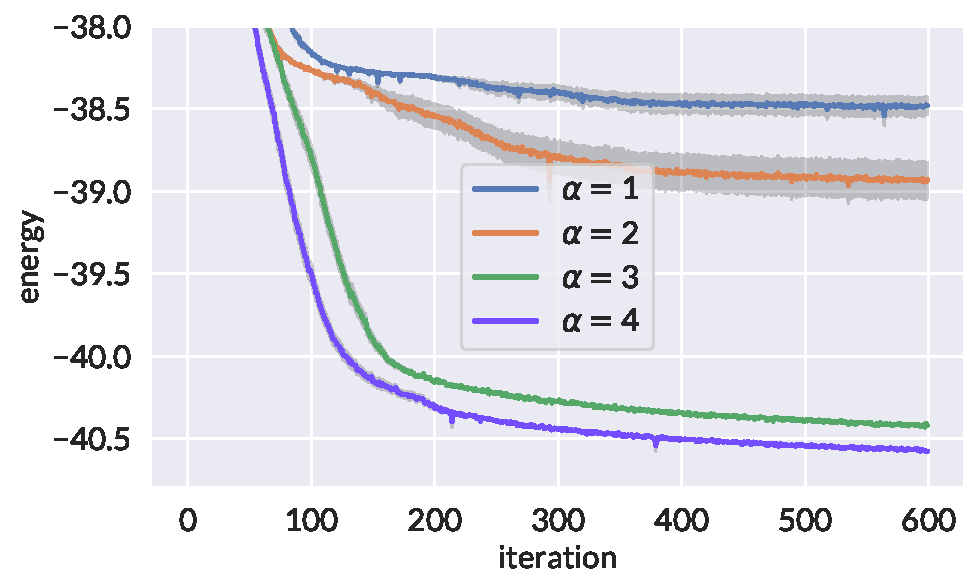
\includegraphics[width=0.7\textwidth]{figures/chapter3/energyvsepoch.pdf}
		\caption{The approach towards the optimal NQS ground-state wavefunction for the $Z^2/Z$ model measured through its energy as a function of learning epoch for $\alpha=1, 2, 3, 4$ for the value $\lambda=0.948, \omega=0$. Considering the $\alpha=1$ result an outlier, one sees an improved convergence as the number of hidden nodes $\alpha$ is increased. The average over 50 initial conditions is given as well as the standard error computed using bootstrap over 500 resamples.
		}
		\label{fig:DeltaE-gs}
	\end{figure}
	
	In this finite size system, there is no true instaneous phase transition, but its incipience is clearly visible in both the specific heat and the development of a finite order parameter for the registry symmetry. Fig.\ref{fig:regCv2fields} illustrates this. We clearly see the incipient second order phase transition as predicted for this model in \cite{Bukva:Registry}.
	\begin{figure}[t]
		\centering
		\mbox{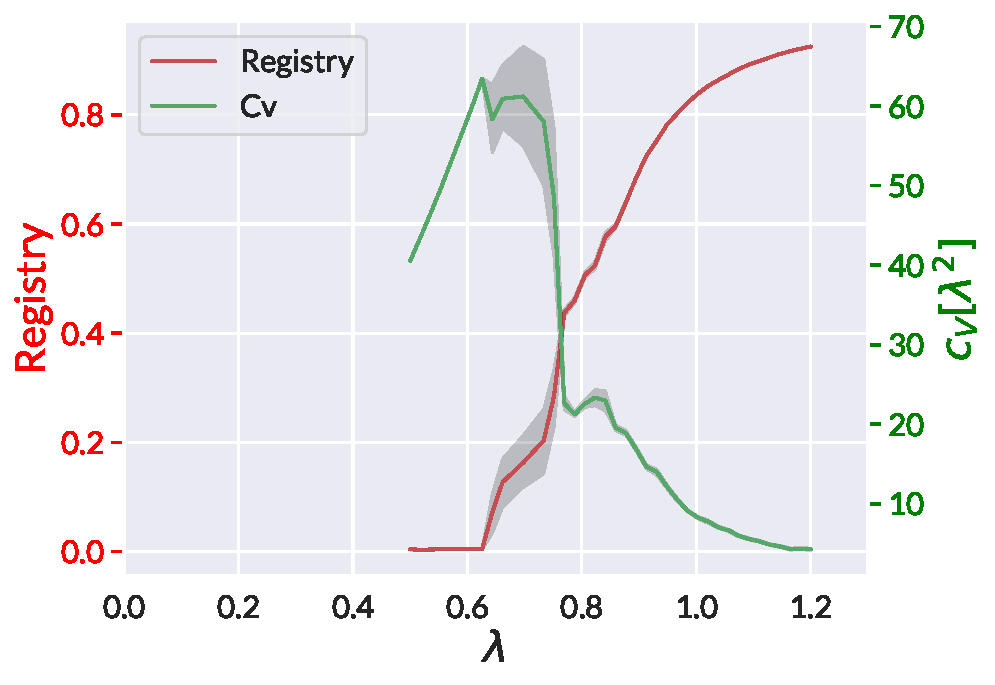
\includegraphics[width=0.33\textwidth]{figures/chapter3/2FieldsCVReg.pdf}
			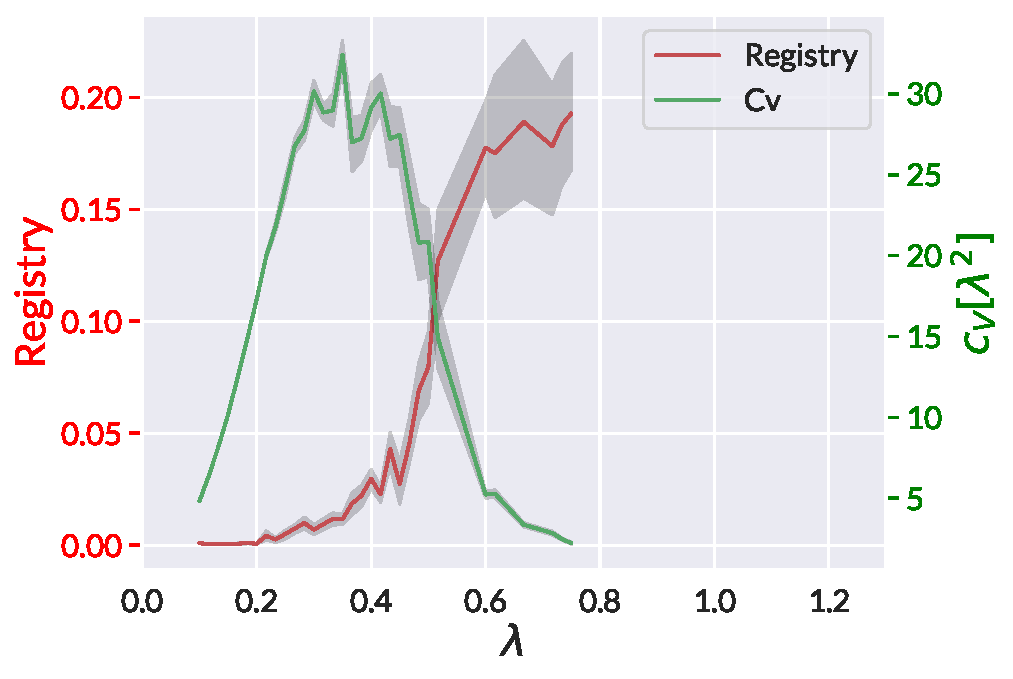
\includegraphics[width=0.33\textwidth]{figures/chapter3/3FieldsCVReg.pdf}
			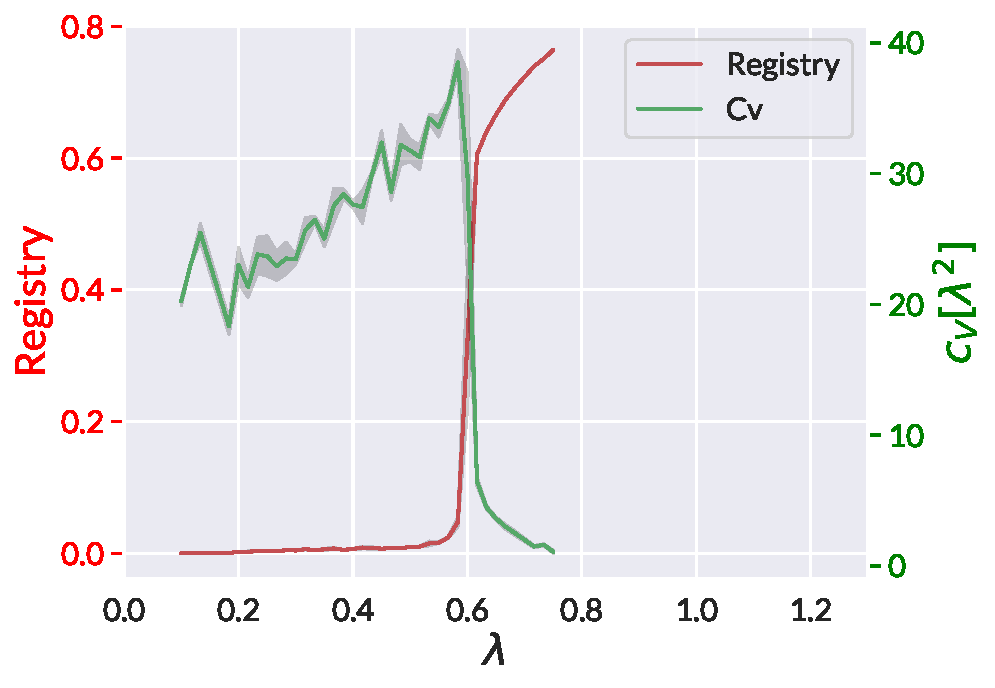
\includegraphics[width=0.33\textwidth]{figures/chapter3/4FieldsCVReg.pdf}}
		\caption{The specific heat $c_V=\frac{\partial \langle E\rangle_{NQS}}{\partial \lambda}$ (green) and registry order parameter $\langle{\cal O}_n\rangle =\langle\sigma_1^{n-1}\ldots\sigma_n^{n-1}\rangle_{NQS}$ (red) for the $Z_2^n/Z_2$ gauge theory for $n=2,3,4$ for $\omega=0$ as a function of $\lambda$ determined from the NQS wavefunction for $\alpha = 3$. The mean and standard deviation after are computed using bootstrap.  
		}
		\label{fig:regCv2fields}
	\end{figure}
	
	We can now test how entanglement also in  2D systems becomes denser {\em both} as we approach the critical point, {\em and} as we increase the number of degrees of freedom analogous to the central charge in 1D systems. Fig.\ref{fig:allEE} gives our results of the entanglement between $2/3$ and $1/3$ of the system. In the case of $3 \times 3$ system, dividing system exactly in half is not possible, the method we opted out for is the divisions along the secondary diagonal as in the Fig.\ref{fig:division}.
	\begin{figure}[t]
		\centering
		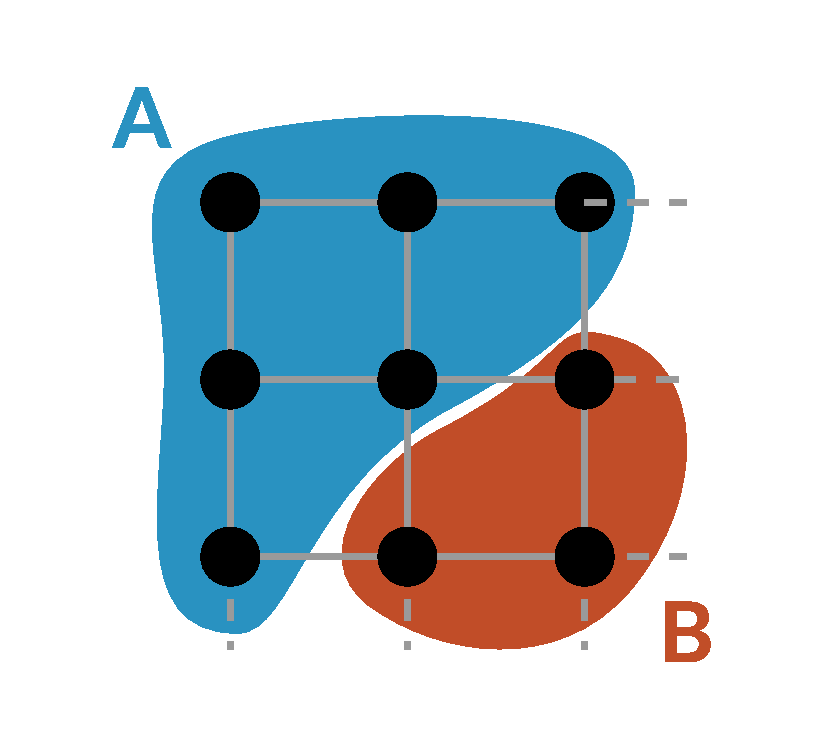
\includegraphics[width=0.35\textwidth]{figures/chapter3/latticeDivision.pdf}
		\caption{Illustration of the system division for a $3 \cross 3$ lattice used in our computations.}
		\label{fig:division}
	\end{figure}
	
	\begin{figure}[t]
		\centering
		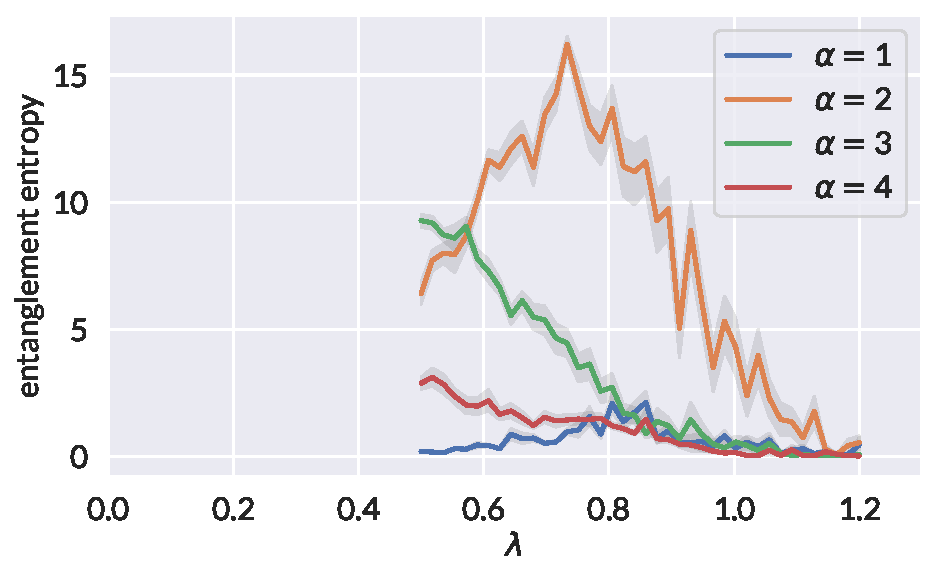
\includegraphics[width=0.33\textwidth]{figures/chapter3/EE_Ntwo.pdf}%
			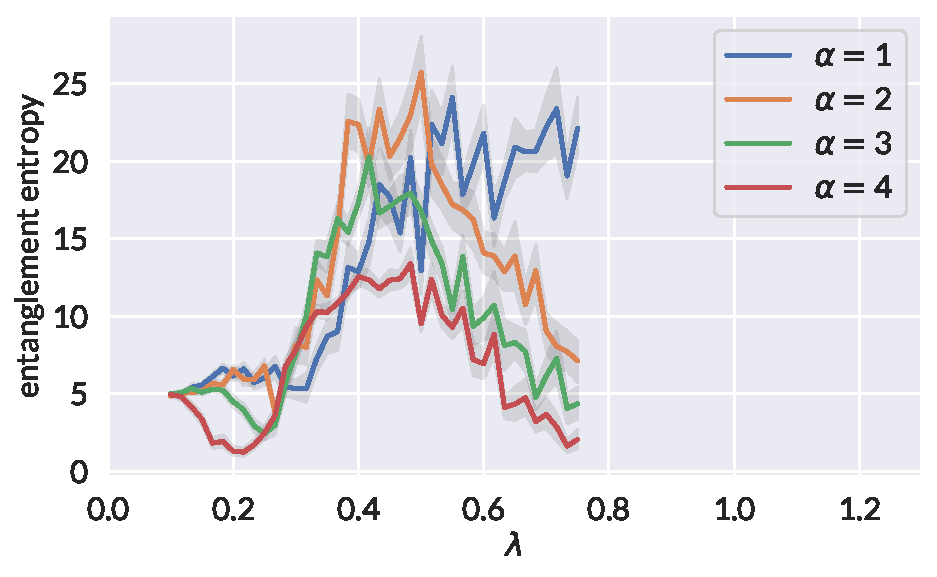
\includegraphics[width=0.33\textwidth]{figures/chapter3/EE_Nthree.pdf}%
			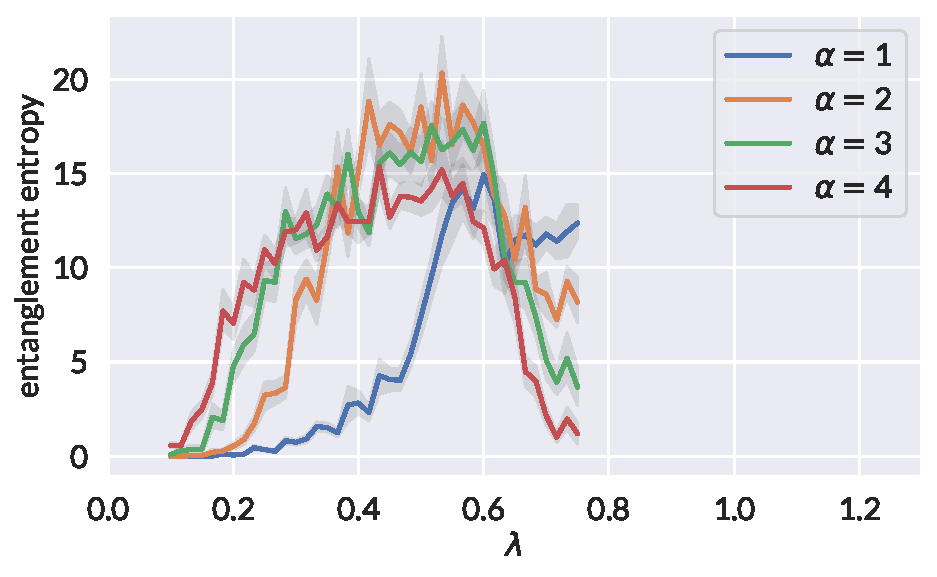
\includegraphics[width=0.33\textwidth]{figures/chapter3/EE_Nfour.pdf}\\
		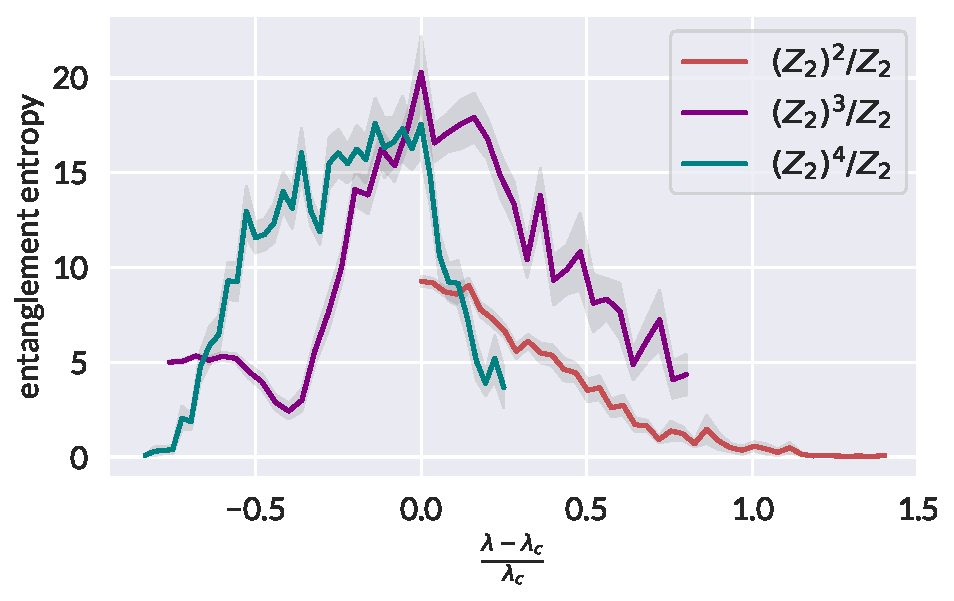
\includegraphics[width=0.33\textwidth]{figures/chapter3/EE_all_fieldsA3.pdf}%
			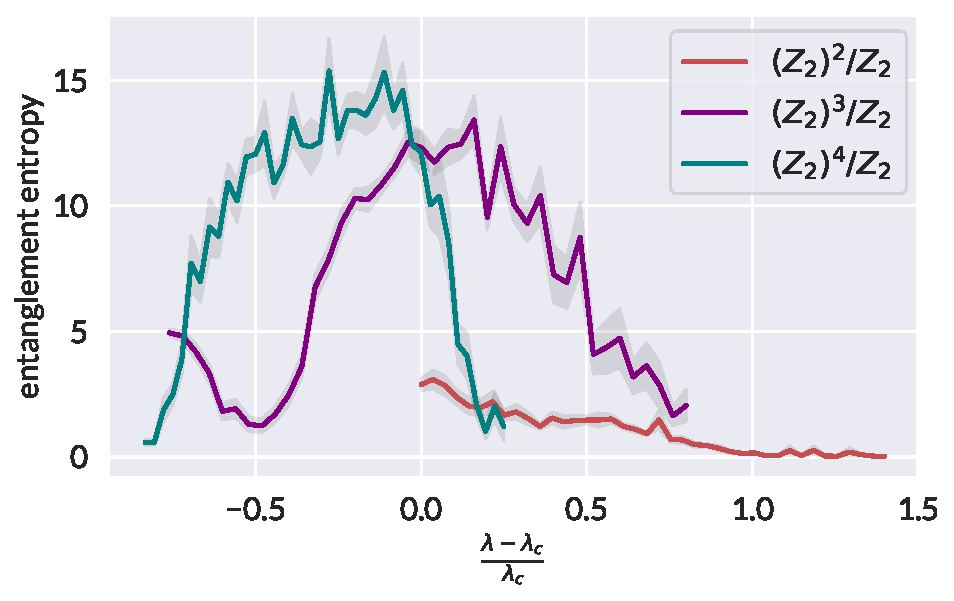
\includegraphics[width=0.33\textwidth]{figures/chapter3/EE_all_fieldsA4.pdf}\\
		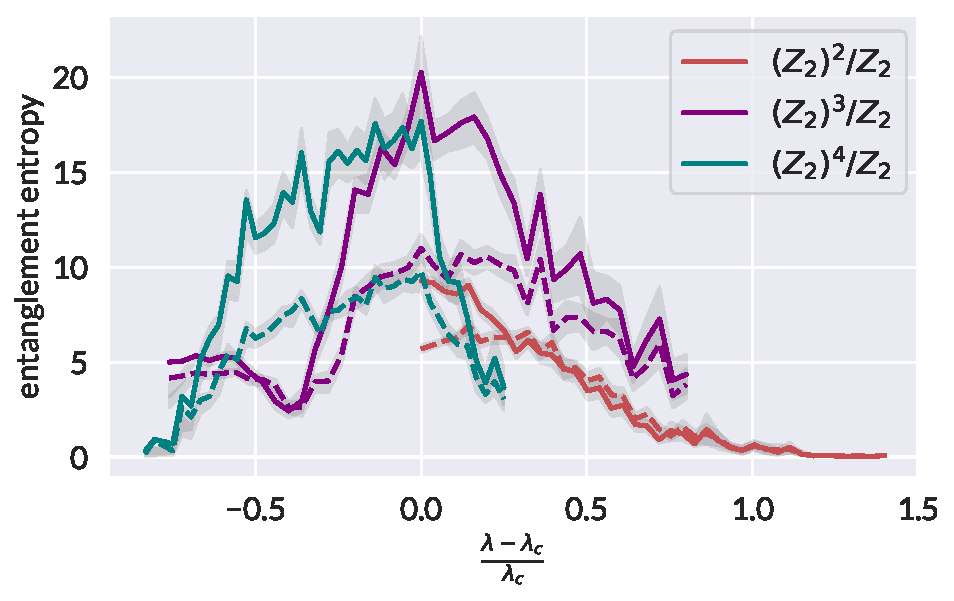
\includegraphics[width=0.33\textwidth]{figures/chapter3/EE_alpha_four_diffNsamples.pdf}
		\caption{The entanglement entropy $S_{2/3}$ of $2/3$ of the $3 \times 3$ system entangled with the other 1/3 for the $N_{\text{red.}}=10^4$ truncated (see text) NQS groundstate of $Z_2^n/Z_2$ gauge theories averaged over 50 initial conditions. The top row shows the dependence on the number of hidden variables as a function of $\lambda$ for $N_{\text{red.}}=10^4$: 
			Left is the result for $n=2$ for $\alpha=1,2,3,4$; middle for $n=3$; right for $n=4$. This estimates the error in the entanglement entropy. The middle
			row shows the dependence on $n$ rescaled to $\lambda_{\text{red.}} =\frac{\lambda-\lambda_c}{\lambda_c}$; left for $\alpha=3$, right for $\alpha=4$ for $N_{\text{red.}}=10^4$. No discernible increase in the entanglement entropy as a function of $n$ is seen. The bottom row shows the dependence on $N_{\text{red.}}=10^4$ (solid line) and $N_{\text{red.}}=10^3$ (dashed line).}
		\label{fig:allEE}
	\end{figure}
	Fig.\ref{fig:allEE} and specifically the middle row of Fig.\ref{fig:allEE} shows the results of the entanglement entropy for the sequence of $Z_2^n/Z_2$ theories as a function of the relative coupling $\lambda-\lambda_c/\lambda_c$ w.r.t. the criticial point.
	Initially the entanglement entropy does increase when going from 2 to 3 fields, but then stays the same when we added another 4th field. Though the numerical results are not super smooth, and there is a slight increase for $\alpha=4$, we expect a linear increase and this is clearly not there. There are several possible explanations for this. One is that finite size effects due to computational limitations do have a direct impact. This cannot be ruled out, but the fact that the entanglement entropy does not change much with the increase in $\alpha$ suggests otherwise. Already $\alpha=1$ appears sufficient to represent all the entanglement in the system. Another possible explanation for the relation between entanglement entropy and the number of matter fields is that increasing number of fields would require an increase in the $N_{\text{red.}}$. From the right figure in the bottom row of Fig.\ref{fig:allEE} we see that increase of $N_{\text{red.}}$ lead to the increase in the entanglement entropy. We are again computationally limited here as a further increase in the number of required states would cause memory issues. 	
	
	\section{Discussion}
	\label{sec:conclusion}
	Having presented our results, we must leave a verification whether entanglement entropy scales with the number of degrees of freedom also at a 2D critical point an open question. Surprisingly, within the limitations of our numerics in the $Z_2^n/Z_2$ sequence of models we studied this appears not to be the case. We cannot fully rule out that a technical/computational limitation is the cause, but we have performed extensive tests and the code faithfully reproduces the known 1D results (see Appendix). One possibility to overcome computational limitations is to move away from the traditional Monte Carlo sampling and using more direct approach like equivariant flow-based sampling \cite{Kanwar_2020} or generative models \cite{medvidovic2021generative}. We leave this for future research.
	
	\section*{Acknowledgments}

	We are especially grateful to Giuseppe Carleo and Matija Medvidovi\' c for their help in setting up NQS for gauged models.
	We thank Jan Zaanen for discussions and his insistence that this should be tested in models with $d>1$.
	This research was supported 
	in part by the Dutch Research Council
	(NWO) project 680-91-116 ({\em Planckian Dissipation and Quantum Thermalisation: From
		Black Hole Answers to Strange Metal Questions.}) and
	by the Dutch Research
	Council (NWO)/Ministry of Education.
	
	\section{Appendix}
	\subsection{NQS States and Entanglement for 1D transverse field Ising Model}
	Given that we have such an unexpected and curious result, it behooves an in depth exhibition of the validity of our approach.
	Here we compute the known entanglement entropy in a 1D transverse Ising model using exactly the same algorithm.
	These results agree with the theoretical expectation as well as the numerical NQS results of \cite{Shi_2019}.
	We have parametrized the 1D transverse field Ising model Hamiltonian analogous to Eq.(\eqref{eq:gaugeHamiltonian})
	\begin{align}
		H_{\text{TI-1D}} = &-\sum_{\vec{r}} \sigma_1(\vec{r})
		-\lambda \sum_{\vec{r}, \mu} \sigma_3(\vec{r})\sigma_3(\vec{r}+\hat{e}_\mu)
	\end{align}
	and use a $N=16$ site system
	with periodic boundary conditions.
	The results are on Fig.\ref{fig:TI-1D}. One sees the increase in entanglement as one approaches the critical value $\lambda_c=XX$ consistent with the notion of dense entanglement. 
	\begin{figure}[H]
		\centering
		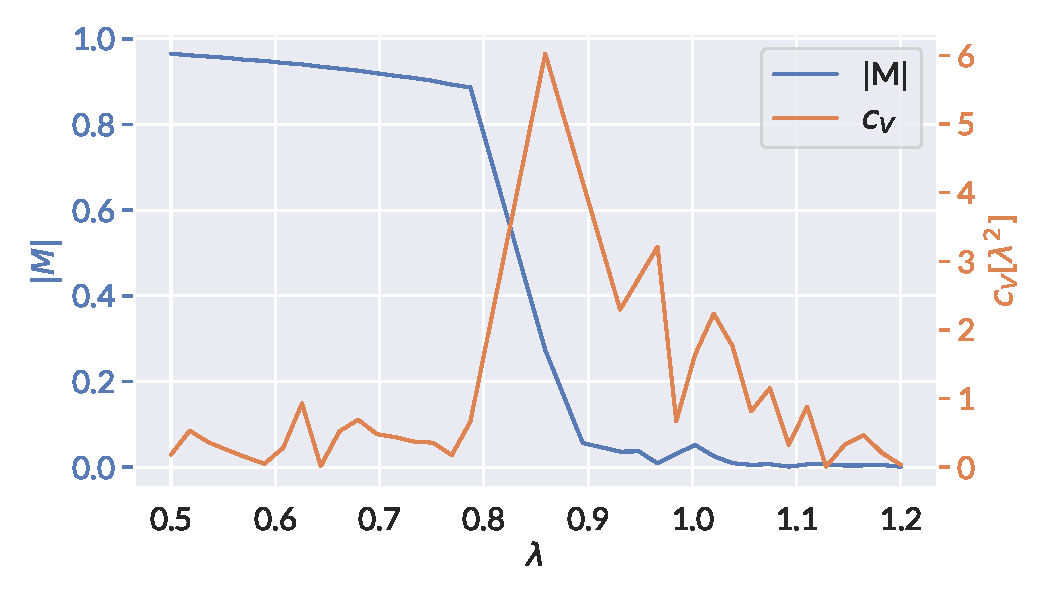
\includegraphics[width=0.4\textwidth]{figures/chapter3/IsingMagCv.pdf}
		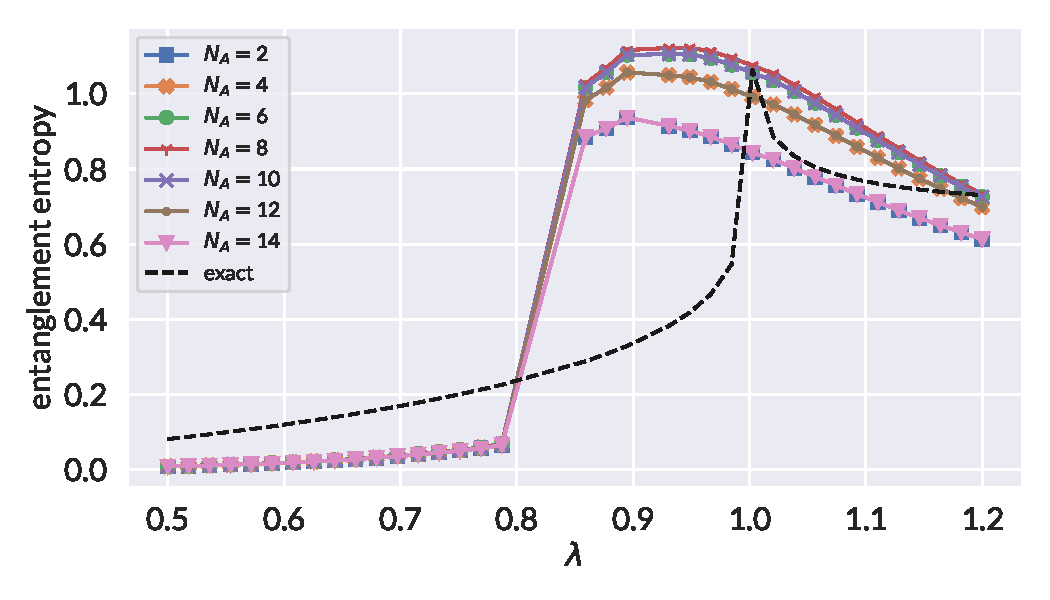
\includegraphics[width=0.4\textwidth]{figures/chapter3/IsingEE.pdf}
		\caption{Left: The specific heat and $Z_2$ order parameter of the 1D Ising model as a function of $\lambda$.
			Right: The entanglement entropy both as a function of $\lambda$ and as a function of boundary site $s=2,4,6,8,10,12,14$ between subsystem $A$ and subsystem $B$ (the boundary site is the last site that is included in $A$.). The dashed line is the CFT result in the continuum limit.}
		\label{fig:TI-1D}
	\end{figure}
		%\chapter{Criticality versus Uniformity in Deep Neural Networks}
\label{ch:edgeofchaos}

\section*{Attribution}
This paper has been previously published as a preprint on arXiv and has been submitted to Journal of Machine Learning Research for publications, and it is currently under the editorial review, under the title \textbf{\textit{Criticality versus uniformity in deep neural networks}}, together with Jurriaan de Gier,  Kevin T. Grosvenor, Ro Jefferson, Koenraad Schalm and Eliot Schwander.\cite{bukva2023criticality}

\section*{Abstract}
Deep feedforward networks initialized along the edge of chaos exhibit exponentially superior training ability as quantified by maximum trainable depth. In this work, we explore the effect of saturation of the tanh activation function along the edge of chaos. In particular, we determine the line of uniformity in phase space along which the post-activation distribution has maximum entropy. This line intersects the edge of chaos, and indicates the regime beyond which saturation of the activation function begins to impede training efficiency. Our results suggest that initialization along the edge of chaos is a necessary but not sufficient condition for optimal trainability.

\section{Introduction}
Over the past decade or so, deep learning has emerged as one of the most powerful tools for processing and analyzing data, and has proven successful on an increasingly wide range of computational challenges. These remarkable feats include highly accurate image classification \cite{NIPS2012_c399862d}, advanced generative modelling of images \cite{2021arXiv210212092R}, natural language processing \cite{2020arXiv200514165B}, accurate protein structure predictions \cite{Jumper:2021wp}, and besting humans in a wide range of games \cite{Schrittwieser:2020ti}. Key to these neural networks' success is the extremely large number of parameters---generally speaking, the \emph{expressivity} of a neural network increases with depth \cite{2016arXiv160605336R}. Expressivity refers to the range of functions that a network can approximate, with the network being understood as simply a function from the space of inputs to the space of outputs. However, the price we must pay for larger and more powerful networks is that they are more difficult to train; for example, the risk of vanishing or exploding gradients is exacerbated with depth \cite{geron2019hands}. Hence, an improved understanding of how the network parameters impact trainability is highly valuable, as even small improvements in the initialization of deep neural networks can make intractable problems tractable.

In this work, we study trainability in deep random feedforward neural networks. Such networks are frequently used in the literature due to their analytical tractability: the phase space is two-dimensional and parameterized by the variances of the initial  weight and bias distributions: $\sigma_w^2$ and $\sigma_b^2$.\footnote{As is standard in the literature, we restrict to zero-mean networks, as initializing with a small non-zero mean does not qualitatively change our results.} This makes them useful models for investigating general features of deep networks. In particular, we will be concerned with the behavior of the pre- and post-activations, in terms of both their distributions as well as the accuracy of the network on 
a classic image classification task, namely MNIST (numerical digit recognition) and CIFAR-10 (colored images, which we convert to grayscale).

More specifically, we build on previous work \cite{arxiv.1606.05340,2016arXiv161101232S} which demonstrated the presence of an order-to-chaos phase transition in this class of deep networks. Intui\-tively, correlations in the input that we wish to learn are exponentially suppressed with depth in the ordered (analogously, low-temperature) phase, and washed-out by noise in the chaotic (high-temperature) phase; these two phases are characterized by vanishing or exploding gradients, respectively. The boundary between these two phases is a critical line called the \emph{edge of chaos},\footnote{Technically, this should be called the edge of stability, but we will use edge of chaos synonymously with criticality for consistency with the literature.} which is a continuous phase transition characterized by a diverging correlation length $\xi$ for the layer-to-layer two-point function of the neurons. Since the correlation length sets the depth scale at which information can propagate, this theoretically enables networks of arbitrary depth to be trained at criticality (more generally, networks are trainable provided their depth does not exceed the scale set by $\xi$). In other words, the deeper the network, the closer one must lie to the edge of chaos; this was demonstrated in \cite{2016arXiv161101232S} along a slice of parameter space at bias variance $0.05$ and weight variance ranging from 1 to 4, and subsequently generalized/corroborated in, e.g., \cite{arxiv.1806.05393,arxiv.1806.05394,Erdmenger:2021sot}

Several questions naturally arise from the above work. First, given that the network parameters will evolve under training in order to minimize the specified cost function and, in particular, develop interdependencies, why does the choice of initialization have such a decisive effect on network performance?\footnote{In other words, why does the network remain near the initialization regime (e.g., the edge of chaos) as it evolves?} Indeed, it was observed in \cite{Erdmenger:2021sot} that the hidden-layer pre-activation distributions (as quantified by their variance) rapidly approach some asymptotic value within 10 or fewer layers, and then remain relatively unchanged for arbitrarily many additional layers. We corroborate this fact at the level of the post-activation in fig. \ref{fig:postevol} of appendix \ref{app:postevol}.

Second, what role does the particular distribution of post-activations in a given layer play in determining network performance? For example, the activation function considered in \cite{2016arXiv161101232S} is hyperbolic tangent, which we adopt henceforth. When $\sigma_{b}^{2} \ll 1$ and $\sigma_{w}^{2} \lesssim 1$, the pre-activations $z$ of the hidden layers are approximately Gaussian-distributed with small variance (cf. \eqref{eq:varrecursion}). In this case, $\tanh(z)\approx z$, so the network behaves like a linear network. These are quite restrictive, being incapable of representing functions whose output data are non-linearly separable and cannot be generated by a combination of linearly separable data. In the opposite extreme, for large values of $\sigma_{w}^{2}$ and $\sigma_{b}^{2}$, the pre-activation variance becomes so large that the post-activation distribution becomes peaked at $\pm1$. In other words, large pre-activation variance saturates the tanh, causing it to behave like a discrete step-function. One expects this regime to also impair trainability, since the gradients on which the backpropagation algorithm depends become vanishingly small everywhere except near the origin.\footnote{Recall that the updates to the weights and biases under gradient descent contain products of the derivatives of the activation functions in all higher layers.} Thus, it seems that one should seek to remain somewhere between these two extremes. Quantifying this is one of the main motivations for the present work.

In particular, note that in both the linear and the saturation regimes, one expects the expressibility of the network to be poor. In contrast, between these extremes lies a region in which the post-activation distribution is approximately uniform, and hence we might expect the expressibility of the network to be maximized at this point. To see this, recall that the uniform distribution has maximum entropy, which measures the number of possible states any particular system can have; a step function, in contrast, can only store a single bit of information, and hence has a low entropy of $\ln2$. This leads to the conjecture that networks whose internal distributions are approximately uniform, i.e., maximally entropic, have higher expressibility, and hence might enjoy a performance advantage. Of course, given approximately Gaussian pre-activations, the post-activation distribution of tanh cannot be exactly uniform, but we can quantify the degree of uniformity via the relative entropy (defined below). In fact, we will show that there is a \emph{line of uniformity} on the $(\sigma_w^2, \sigma_b^2)$ phase space along which the post-activation distribution is as uniform as possible. This line intersects the aforementioned edge of chaos (see fig. \ref{fig:loueoc}), and the relative importance of lying near this line is the primary question we shall explore below. 

We shall begin by deriving an expression for the line of uniformity, defined by the condition that the distribution of the final hidden layer minimizes the relative entropy with respect to the uniform distribution. The computation uses many of the same ingredients as \cite{2016arXiv161101232S}, and the interested reader is encouraged to turn there for more background. We then examine proximity to this line in relation to the edge of chaos considered in previous works. 

We find that for deep networks away from the edge of chaos, the exponential suppression dominates, and no benefit from uniformity is observed. However, along the edge of chaos -- where the suppression is only polynomial -- we find a relatively sharp fall-off in the post-training accuracy to the right of the line of uniformity. The location of this fall-off depends on the learning rate, since decreasing the learning rate can increase the final accuracy, but at the cost of additional computing time (see fig. \ref{fig:edge of chaos-drop-off-beyond-lou}). This suggests that criticality is a necessary but not sufficient condition for optimal trainability. 

This dependence on other hyperparameters illustrates that optimal trainability is not just a matter of final accuracy but also of efficiency, i.e., how quickly the final accuracy is reached. Since computational limits exist, we shall rely on an intuitive notion of efficiency per epochs in addition to accuracy; that is, we consider the accuracy achieved after a fixed number of training epochs. It is conceivable that in the limit of infinite training epochs accuracy differences disappear, so that formally, the configurations are equally good. In a practical sense however, they clearly are not.

Note that there can obviously be very many notions of efficiency depending on which resource(s) one considers most valuable. Here, we are implicitly prioritizing training time, i.e., number of epochs. If one were to put the premium on floating point operations used in training, then one would instead measure efficiency as in \cite{2020arXiv200504305H}. Yet another concept called learning efficiency has to do with how much time it takes to run a learning algorithm and, in particular, how this scales with the size of the input space \cite{2014arXiv1410.1141L}. 

Returning to our main question, to isolate the effects of uniformity \emph{away} from the edge of chaos, we also examine networks which are both shallow (i.e., not yet exponentially suppressed) and narrow (i.e., low expressibility per layer), and confirm that training efficiency, in the sense described above, degrades to the right of the line of uniformity (i.e., away from the origin), though final accuracy need not. In contrast to the edge of chaos, the line of uniformity is not a sharp phase boundary, but it does indicate coarsely the parameter boundary where activation saturation starts to affect training efficiency. This not only establishes the more obvious point that, even in deep random feedforward toy models on the edge of chaos, backpropagation training depends sensitively on activation function choice, as earlier emphasized in \cite{2018arXiv180508266H,pmlr-v97-hayou19a}, but also that for a given activation function choice there are optimal points or regions on the edge of chaos itself.

\section{The line of uniformity}
We can estimate the location of the line of uniformity by capitalizing on the fact that wide networks, with a large number $N$ of neurons in each hidden layer, are approximate Gaussian processes. At finite $N$, the neurons in a given layer are not independent due to their shared dependence on the neurons in the previous layer. Physically however, the non-Gaussianities that can be seen by marginalizing over the previous layer(s) can be thought of as interactions that are $1/N$ suppressed \cite{Roberts:2021fes,Grosvenor:2021eol}. Hence, in the limit $N\rightarrow\infty$, the distribution of pre-activations becomes Gaussian, essentially by the central limit theorem. This greatly simplifies the analysis, and is the reason for the widespread use of such models in previous studies, including \cite{2016arXiv161101232S}.\footnote{One will often see the phrase ``mean-field theory'' used in place of the central limit theorem in this context; however, as pointed out in \cite{Grosvenor:2021eol}, this is not technically correct, and mean-field theory does not necessarily correspond to the $N\rightarrow\infty$ limit.}

Thus, at large-$N$, the distribution of pre-activations $z$ for any hidden layer takes the form
\begin{equation} \label{eq:pre}
	p (z ; \sigma^2 ) = \frac{1}{\sqrt{2 \pi} \, \sigma} \, e^{- \frac{z^2}{2 \sigma^2}}~,
\end{equation}
where $\sigma^2$ is the variance, and we assume the mean $\mu=0$ since adding a small finite mean does not qualitatively change our results. If the activation function $\phi (z)$ is one-to-one and once-differentiable, then the distribution of post-activations $x$ will be given by
%
\begin{equation} \label{eq:postgeneral}
	p_{\phi} (x ; \sigma^2 ) = \frac{1}{\sqrt{2 \pi} \, \sigma\,\phi' \bigl( \phi^{-1} (x) \bigr)} \, e^{- \frac{\phi^{-1} (x)^2}{2 \sigma^2}}~.
\end{equation}
%
Concretely, for $\phi (z) = \tanh (z)$, this yields
%
\begin{equation} \label{eq:ppost}
	p_{\phi} (x; \sigma^2 ) = \frac{1}{\sqrt{2 \pi} \, \sigma (1 - x^2 )} \, e^{- \frac{\rm{arctanh} (x)^2}{2 \sigma^2}}~,
\end{equation}
%
with $x\in[-1,1]$. The corresponding variance is given by
%
\begin{equation} \label{eq:varpost}
	\sigma_{\phi}^{2} = \int_{-1}^{1}\mathrm{d} x \, x^2 \, p_{\phi} \bigl( x ; \sigma^2 \bigr)~.
\end{equation}
%
%

As mentioned above, we quantify the uniformity of the post-activation distribution $p_\phi$ by the relative entropy or Kullback-Leibler divergence with respect to the uniform distribution $p_\mathrm{uni}$,
\begin{equation}
	S(p_\mathrm{uni}||p_\phi)
	%\coloneqq
	=\int_{-1}^1\!\mathrm{d} x\;p_\mathrm{uni}(x)\ln\frac{p_\mathrm{uni}(x)}{p_\phi(x)}~.
\end{equation}
Substituting in \eqref{eq:ppost} and $p_\mathrm{uni}=\tfrac{1}{2}$, this yields
\begin{equation} \label{eq:relent}
	S( p_{\rm{uni}} || p_{\phi} ) = \frac{1}{2}\ln(8\pi\sigma^2)+\frac{\pi^2}{24 \sigma^2}-2~.
\end{equation}
%
This has a minimum at
%
\begin{equation} \label{eq:sigmamin}
	\sigma_{\rm{min}}^{2} = \frac{\pi^2}{12} \approx 0.822~.
\end{equation}
%

Therefore, we wish to find the set of points $(\sigma_w^2,\sigma_b^2)$ at which the variance of the final hidden layer is $\sigma_\mathrm{min}^2$; this  will define the line of uniformity. To proceed, we use the recursion relation
%
\begin{align} \label{eq:varrecursion}
	\sigma_{\ell}^{2} = \sigma_{w}^{2} \, \sigma_{\phi , \ell -1}^{2} + \sigma_{b}^{2}~,
\end{align}
%
which follows from the large-$N$ condition discussed above (i.e., the neurons on any given layer can be treated as i.i.d. random variables). Note that this is exactly the same as eq. (3) of \cite{2016arXiv161101232S}, where our $\sigma_{\ell}^{2}$ is their $q_{aa}^{\ell}$ and our $\sigma_{\phi, \ell -1}^{2}$ is the corresponding integral expression.\footnote{Explicitly, the variance can be written as $\sigma_{\phi}^{2} = \int \mathcal{D} z \, \bigl[ \phi ( \sigma z ) \bigr]^2$, where $\mathcal{D}z=\tfrac{\mathrm{d} z}{\sqrt{2\pi}}e^{-\frac{z^2}{2}}$ is the standard Gaussian measure.\label{ft:gauss}} This recursion relation ostensibly requires the variance of the first hidden layer, $\sigma_1^2$, as an input. However, it turns out that \eqref{eq:varrecursion} quickly converges to a fixed value $\sigma_{*}^{2}$, which (by definition) is a function of $\sigma_{w}^{2}$ and $\sigma_{b}^{2}$, but not of $\sigma_{1}^{2}$:
%
\begin{equation} \label{eq:sigmastar}
	\sigma_{*}^{2} = \sigma_{w}^{2} \, \sigma_{\phi , *}^{2} + \sigma_{b}^{2},
\end{equation}
%
where $\sigma_{\phi, *}^{2}$ is $\sigma_{\phi}^{2}$ evaluated at $\sigma_{*}^{2}$; see \cite{arxiv.1606.05340} for further discussion of this convergence. In appendix \ref{app:postevol}, we have demonstrated numerically that the corresponding post-activation distribution indeed converges rapidly to one which depends only on the initialization point $(\sigma_w^2, \sigma_b^2)$.

Now, consider a fixed value of $\sigma_*^2$ (and hence also of $\sigma_{\phi , *}^{2}$). Then we can consider \eqref{eq:sigmastar} as an expression for $\sigma_b^2$ as a function of $\sigma_w^2$, which defines a line in phase space of the form
\begin{equation} \label{eq:fixedsigmastar}
	\sigma_{b}^{2} = \sigma_{*}^{2} - \sigma_{\phi , *}^{2} \, \sigma_{w}^{2}.
\end{equation}
%
where $\sigma_*^2$ is the $y$-intercept, and $- \sigma_{\phi , *}^{2} $ is the slope. Since the relative entropy \eqref{eq:relent} of the final hidden layer is only a function of its variance, the lines of constant $\sigma_*$ given by \eqref{eq:fixedsigmastar} are also lines of constant relative entropy. In particular, the line of uniformity (minimum relative entropy) is given by \eqref{eq:fixedsigmastar} with $\sigma_{*}^{2} = \sigma_{{\rm min}}^{2} = \frac{\pi^2}{12}$, cf. eq. \eqref{eq:sigmamin}. There is no closed-form expression for $\sigma_{\phi,\mathrm{min}}^{2}$, but we can evaluate \eqref{eq:varpost} numerically to obtain $\sigma_{\phi , {\rm min}}^{2} \approx 0.359$. In summary, the line of uniformity (LOU) is given by
%
\begin{equation} \label{eq:lou2}
	{\rm LOU}: \quad \sigma_{b}^{2} = \sigma_{{\rm min}}^{2} - \sigma_{\phi, {\rm min}}^{2} \, \sigma_{w}^{2},
\end{equation}
%
with $\sigma_{{\rm min}}^{2} = \frac{\pi^2}{12} \approx 0.822$ and $\sigma_{\phi, {\rm min}}^{2} \approx 0.359$. In the left panel of fig. \ref{fig:loueoc}, we present a contour plot of the logarithm of the relative entropy. The line of uniformity is the dashed black line---to the left of it, as one approaches the origin, is the linear regime; and to the right, the activation becomes more and more saturated. For comparison, the edge of chaos is the solid black line.
%
\begin{figure}[t!]
	\centering
	\begin{subfigure}{0.5\linewidth}
		\centering
		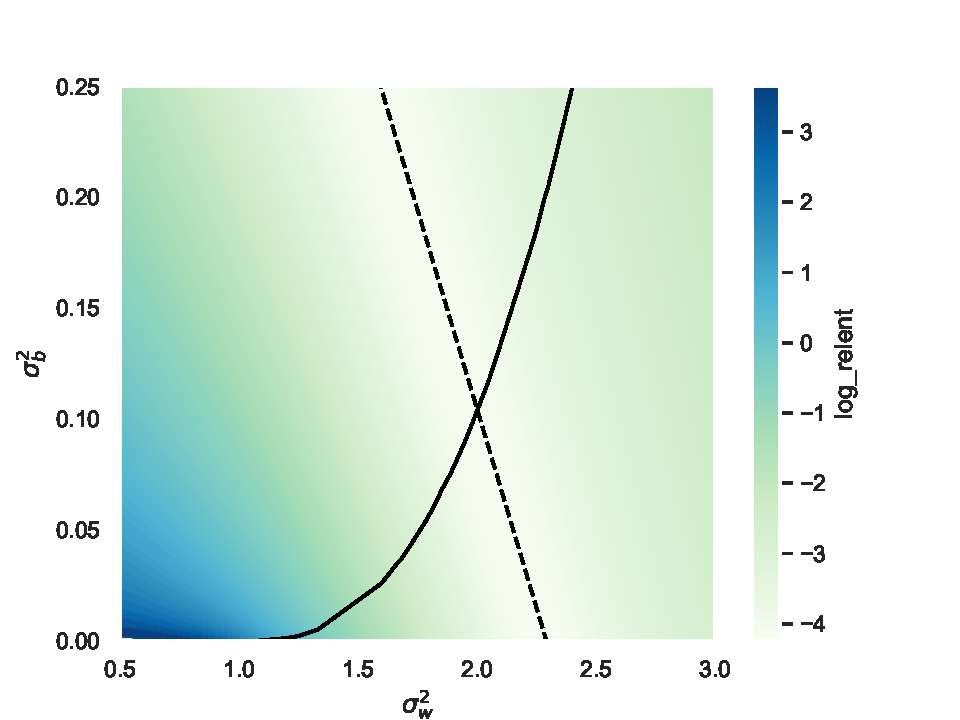
\includegraphics[width=8cm]{figures/chapter4/log_relent_plot_GnBu.pdf}
	\end{subfigure}%
	\begin{subfigure}{0.5\linewidth}
		\centering
		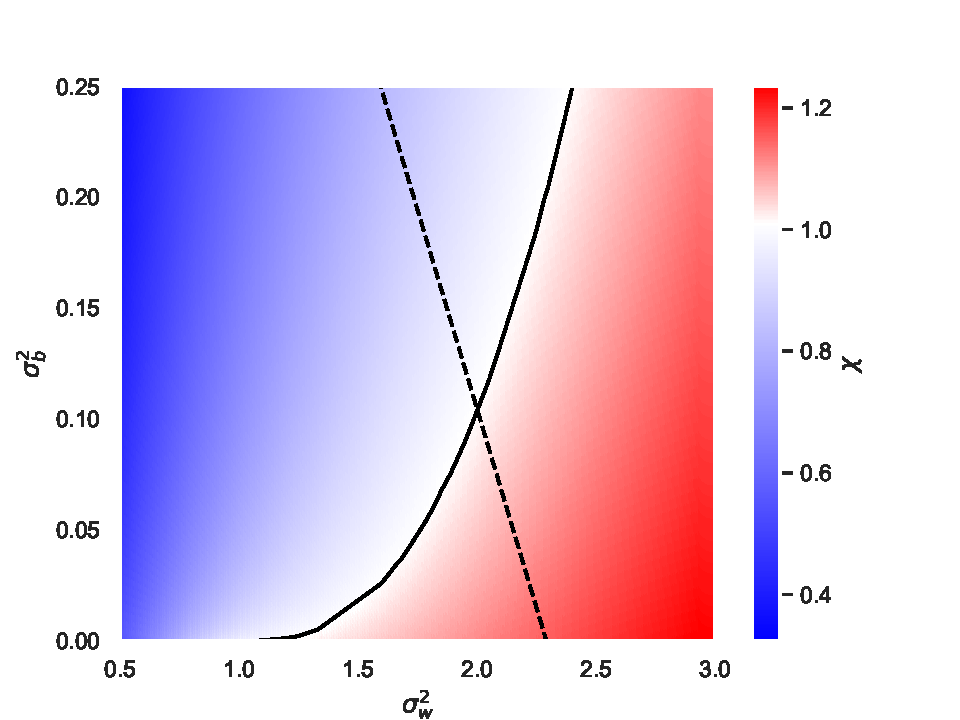
\includegraphics[width=8cm]{figures/chapter4/chi_plot.pdf}
	\end{subfigure}
	\caption{(Left) Contour plot of the logarithm of the relative entropy in the $(\sigma_{w}^{2},\sigma_{b}^{2})$ plane. The dashed line is the line of uniformity---saturation increases to the right of it and linearity increases to the left of it. (Right) Contour plot of $\chi=e^{-1/\xi}$. The ordered/low-temperature phase is shaded blue, while the chaotic/high-temperature phase is shaded red. In both, the solid black line is the edge of chaos, while the dashed black line is the line of uniformity.}
	\label{fig:loueoc}
\end{figure}

\section{The edge of chaos}

The method for computing the edge of chaos as a function of $\sigma_{w}^{2}$ and $\sigma_{b}^{2}$ is described in \cite{arxiv.1606.05340,2016arXiv161101232S}. Once we have $\sigma_{*}^{2}$, as described previously, then we can define the quantities
%
\begin{align} \label{eq:corlength}
	\chi &= \sigma_{w}^{2} \int \mathcal{D} z \, \bigl[ \phi ' ( \sigma_* z ) \bigr]^2, &%
	%
	\xi &= - \frac{1}{\ln \chi},
\end{align}
%
where $\mathcal{D} z$ is the standard Gaussian measure, cf. footnote \ref{ft:gauss}, and $\xi$ is the correlation length mentioned in the introduction (note that this is denoted $\xi_c$ in \cite{2016arXiv161101232S}). 

The meaning of $\chi$ will be discussed in the next paragraph, while the meaning of $\xi$ is as follows: we consider two identical copies of the network and feed them slightly different inputs. Then, we can study the correlation (i.e., covariance) between a neuron in one copy and the same neuron in the second copy as a function of the layer. This correlation will decay exponentially for deeper layers with a characteristic length scale, $\xi$. (Strictly speaking, this is only true in the ordered phase: in the chaotic phase, the quantity $\xi$ is complex-valued and cannot be interpreted as a correlation length). The edge of chaos is defined as the critical point, where the correlation length $\xi$ diverges.

As discussed in more detail in \cite{arxiv.1606.05340, 2016arXiv161101232S}, $\chi$ is obtained as the derivative of the aforementioned covariance with respect to that in the previous layer, and probes the stability of the fixed point when the covariance is unity: $\chi>1$ implies that we approach this point from below (unstable), while $\chi<1$ implies that we approach this point from above (stable).\footnote{See \cite{roCrit} for a pedagogical explanation.} The edge of chaos corresponds to $\chi=1$, where $\xi$ diverges.  

To find the edge of chaos, we can scan over the space of tuples $(\sigma_w, \sigma_*)$ to find those which satisfy the condition $\chi=1$. We then feed these into \eqref{eq:varrecursion} to find the corresponding value of $\sigma_b$. In this manner, we can find arbitrarily many points on the edge of chaos (EOC). Within some finite range of $\sigma_{w}^{2}$ values, we can find a good fit to the EOC. In the range $1 \leq \sigma_{w}^{2} \leq 10$, a good polynomial fit is
\begin{align} \label{eq:eocfit}
	{\rm EOC}: \quad \sigma_{b}^{2} &= \sum_{n=2}^{9} \frac{c_n}{n!} ( \sigma_{w}^{2} - 1 )^n,
\end{align}
with fit coefficients
%
\begin{equation}
	\setlength{\tabcolsep}{5pt}
	\renewcommand{\arraystretch}{1.2}
	\begin{tabular}{ll|ll}
		\hline
		$n$ & $\phantom{-} c_n$ & $n$ & $\phantom{-} c_n$ \\
		\hline\hline
		2 & $\phantom{-} 0.0190$ & 6 & $-1.15$ \\
		%
		3 & $\phantom{-} 0.778$ & 7 & $\phantom{-} 0.769$ \\
		%
		4 & $-1.07$ & 8 & $-0.328$ \\
		%
		5 & $\phantom{-} 1.25$ & 9 & $\phantom{-} 0.0672$ \\
		\hline
	\end{tabular}
\end{equation}
%
Of course, we can reduce the number of fit coefficients needed by reducing the range of $\sigma_{w}^{2}$ values over which we require the fit to be good.

The form of this fit is designed such that it contains the point $( \sigma_{w}^{2} , \sigma_{b}^{2} ) = (1,0)$, and that the edge of chaos has zero slope at this point. We justify these conditions analytically in appendix \ref{app:analytics}. In the right plot in fig. \ref{fig:loueoc}, we present a contour plot of $\chi$. Again, the edge of chaos is drawn as a solid black line and the line of uniformity as a dashed line. The point of intersection of the edge of chaos and line of uniformity is found to be
%
\begin{equation} \label{eq:intersect}
	( \sigma_{w}^{2} , \sigma_{b}^{2} )_{{\rm intersect}} = (2.00, 0.104)~.
\end{equation}
%

\begin{figure*}[t!]
	\centering
	\begin{subfigure}[t]{0.5\textwidth}
		\centering
		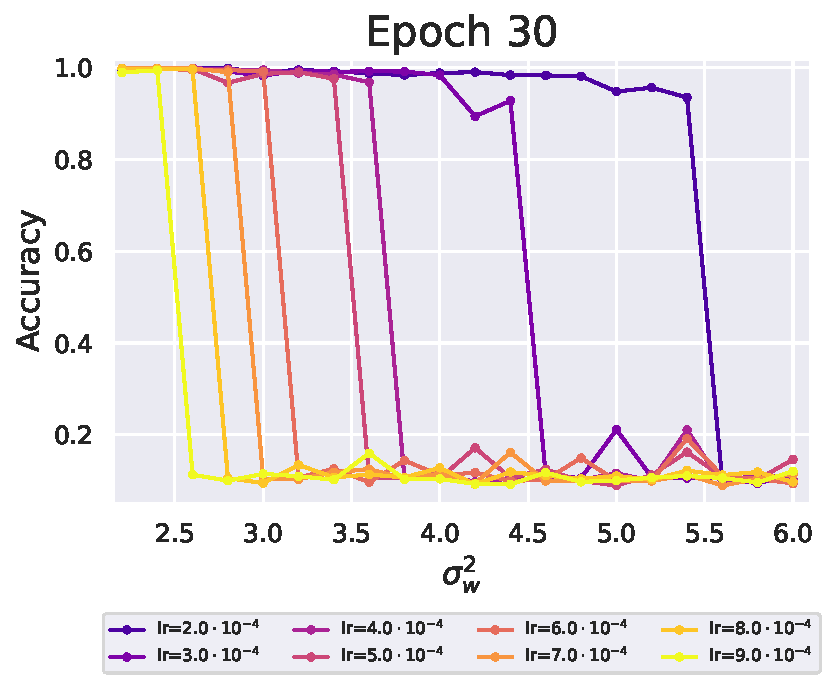
\includegraphics[width=\textwidth]{figures/chapter4/dropOff30EpochSmallerRange.pdf}
	\end{subfigure}%
	\begin{subfigure}[t]{0.5\textwidth}
		\centering
		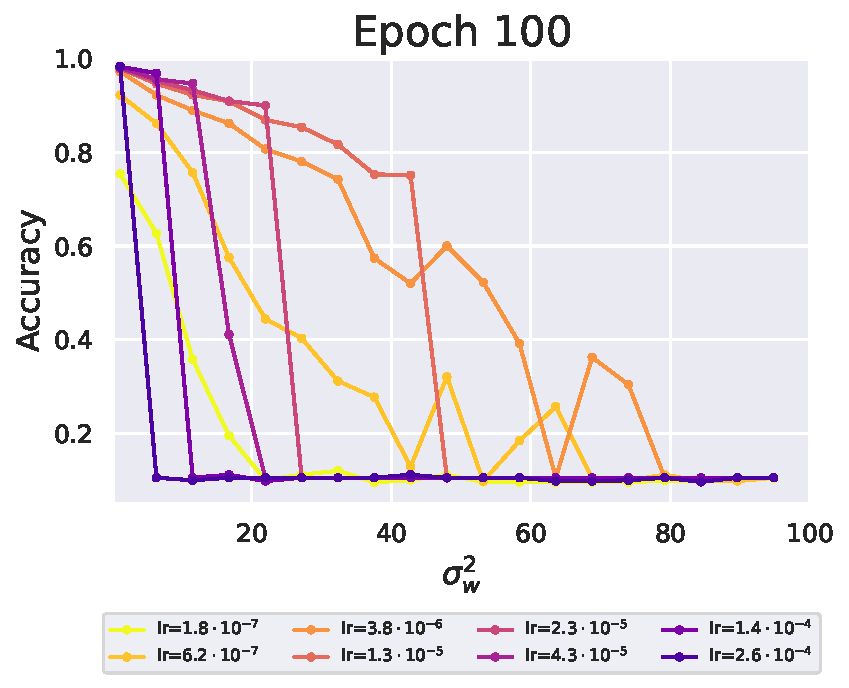
\includegraphics[width=\textwidth]{figures/chapter4/dropOff100Epoch.pdf}
	\end{subfigure}
	\caption{Accuracies on MNIST for distributions of initial weights along the edge of chaos in a deep ($L=100$), wide ($N=784$) neural network with tanh activation function, for a range of learning rates, after 30 epochs (left) and 100 epochs (right). We observe a drop-off in accuracy beyond a value $\sigma_w^2$ which is up to an order of magnitude larger than the point at which the line of uniformity is crossed. For learning rates of the order typically used in the literature, this point is near the intersection of the LOU and the EOC, but moves to higher values of $\sigma_w^2$ for smaller learning rates. When learning rates become extremely small ($r<10^{-5}$), learning becomes highly inefficient, and the drop-off less sharp for the training duration considered. Networks were trained via stochastic gradient descent with batch size 64 and momentum 0.8.} %\ed{Future?: Similar for CIFAR.}
	\label{fig:edge of chaos-drop-off-beyond-lou}
\end{figure*}

\section{The impact of uniformity along the edge of chaos}
To the right of the line of uniformity, neurons begin to saturate the tanh activation function, i.e., approach $\pm1$. This implies that backpropagation based on gradient descent should be less efficient, and hence networks should reach a lower accuracy in a fixed amount of training time. The Google Brain collaboration has already established that at the edge of chaos, learning accuracy is enhanced due to polynomial rather than exponential decay of correlations as a function of network depth \cite{2016arXiv161101232S}. Combining the two insights, optimal learning should therefore take place on the edge of chaos near the line of uniformity. 

To test this hypothesis, we have performed the MNIST image classification task in networks ranging up to a depth of $L=100$ hidden layers at various points along the edge of chaos. The resulting learning accuracy is shown in fig.~\ref{fig:edge of chaos-drop-off-beyond-lou}. We see that this expectation is partially validated. On the left side of the line of uniformity -- but to the right of the linear regime -- all points on the edge of chaos are equally good at learning. But beyond a certain point, which lies to the right of the intersection point \eqref{eq:intersect} of the edge of chaos and line of uniformity, the final accuracy decreases. However, this drop-off point is substantially (up to an order of magnitude) displaced to the right of the intersection point, indicating that the line of uniformity is perhaps better thought of as a region rather than a narrow band, and depends on hyperparameters (such as the learning rate) as mentioned above. Nevertheless, for typical learning rates used in the literature of order $10^{-3}$, such as used in \cite{2016arXiv161101232S}, the drop-off point at approximately $\sigma_{w}^{2} \sim 2.5$ is indeed fairly close to the intersection between the line of uniformity and the edge of chaos at $\sigma_{w}^{2} = 2$. 

We repeated this exercise for the CIFAR-10 image classification task, and present the corresponding results in fig. \ref{fig:EOCdropoffCIFARtanh}. We converted the colored images to grayscale to reduce the input size by a factor of 3. The drop-off in accuracy along the edge of chaos towards larger values of $\sigma_{w}^{2}$ is still present, though the effect is not as dramatic as it is for MNIST. This is not surprising as CIFAR is a much more difficult task than MNIST and so we expect that the saturation of slightly more or fewer neurons will have a much less decisive effect. We note however that in the regime of extremely small learning rates, where training MNIST becomes highly inefficient, the MNIST and CIFAR results appear similar insofar as neither exhibits the obvious sharp drop-off observed for MNIST at the higher learning rates generally used in practice.

\begin{figure*}[!h]
	\centering
	\begin{subfigure}[t]{0.5\textwidth}
		\centering
		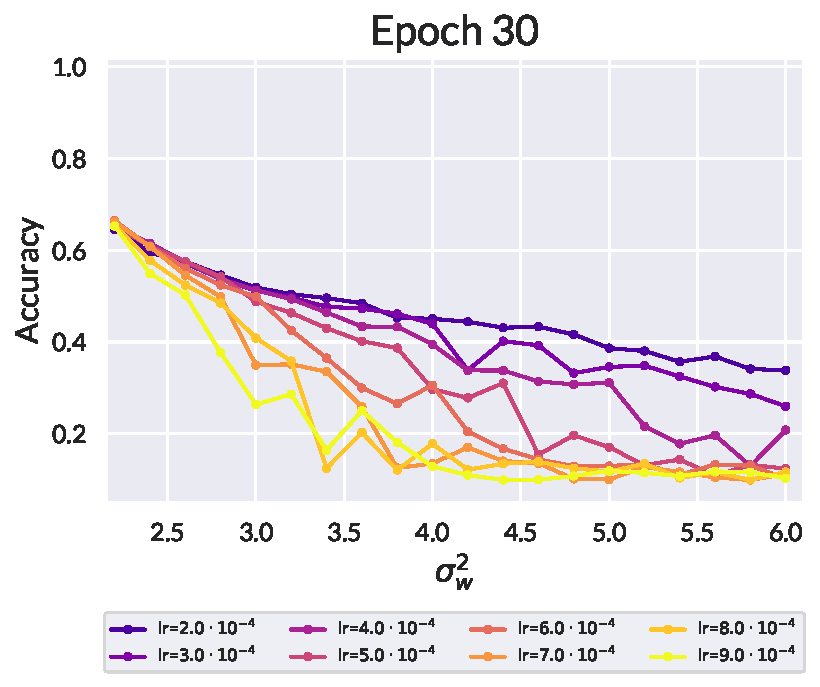
\includegraphics[width=\textwidth]{figures/chapter4/CIFAR-TANH-30Epoch.pdf}
	\end{subfigure}%
	\begin{subfigure}[t]{0.5\textwidth}
		\centering
		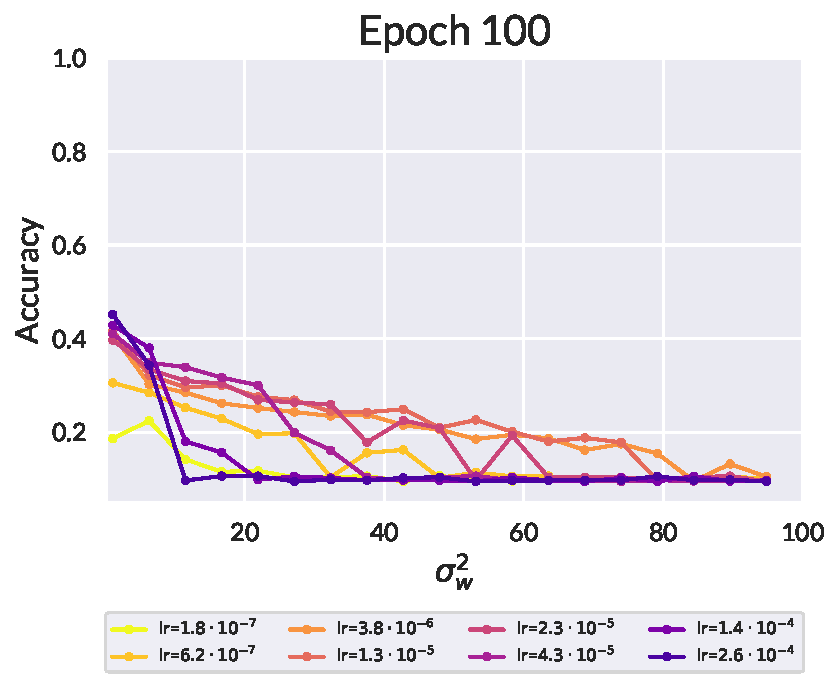
\includegraphics[width=\textwidth]{figures/chapter4/CIFAR-TANH-100Epoch.pdf}
	\end{subfigure}
	\caption{Accuracies on CIFAR-10 for distributions of initial weights along the edge of chaos in a deep ($L=100$), wide ($N=1024$) neural network with tanh activation function, for a range of learning rates, after 30 epochs (left) and 100 epochs (right). The drop-off in accuracy towards higher values of $\sigma_{w}^{2}$ here is much more gradual than the sharp drop-offs observed for MNIST in fig. \ref{fig:edge of chaos-drop-off-beyond-lou} (at all but the lowest learning rates, $r < 10^{-5}$). Networks were trained via stochastic gradient descent with batch size 64 and momentum 0.8.} %\ed{Future?: Similar for CIFAR.}
	\label{fig:EOCdropoffCIFARtanh}
\end{figure*}

Thus, the line of uniformity is not a sharp boundary, unlike the edge of chaos. This is somewhat inherent in its definition, which selects proximity to the uniform distribution of final hidden layer weights as a condition for efficient learning based on the entropic argument given above, but does not specify any particular fall-off behavior. The line of uniformity does, however, give an estimate of where the saturation of the activation function should start to affect learning, and by extension, the point at which saturation of the activation function begins to hinder learning efficiency. To summarize: on the left side of the line of uniformity, the distributions are sufficiently narrow that saturation of the tanh activation function does not occur, and all initial weight distributions along the EOC learn equally well. Conversely, on the right side of uniformity, neurons saturate the activation function and hence hamper learning, even along the EOC. This is our main observation. Importantly, we note that the studies by \cite{2016arXiv161101232S} were performed to the left of the point where the line of uniformity crosses the edge of chaos and hence at optimal efficiency. 

Before moving on to our final set of experiments, we note that the above conclusion is of course specific to saturating activation functions, specifically tanh. This is one motivation for the use of non-saturating activation functions such as ReLU or SWISH, though the unbounded nature of such functions presents its own set of training difficulties. While a similar analysis of uniformity, as quantified by the maximally entropic distribution, for non-saturating activation functions is beyond the scope of this work, a brief inspection of learning efficiency along the EOC for SWISH shows no loss of accuracy in agreement with the absence of saturation effects; see appendix \ref{app:swish}.\footnote{For both SWISH and tanh, the edge of chaos is a line of critical initalizations through phase space, while for ReLU it is only a single point \cite{Roberts:2021fes}.}

\section{Uniformity away from the EOC}
Thus far, we have examined the impact of uniformity on training efficiency along the edge of chaos. Now, we would like to explore whether the line of uniformity still affords training advantages even for networks initialized far from criticality. In attempting to exhibit this however, one quickly finds that the edge of chaos represents a far more dominant effect than the line of uniformity. A close inspection of the learning accuracy of deep (L=300) and wide (N=784) MNIST learning networks shows that there is no discernible difference in learning accuracy away from the edge of chaos: it is simply poor everywhere (see fig. \ref{fig:googleBrain-repro} in appendix~\ref{app:figs}, also \cite{2016arXiv161101232S}.) This can be understood from the form of the correlation functions: away from the edge of chaos, correlations damp exponentially $\sim e^{-L/\xi}$. For a deep network, this exponential damping will erase any finer difference in accuracy results. Along the edge of chaos, the damping is only polynomial and, therefore, the finer difference remains, as seen in fig.~\ref{fig:edge of chaos-drop-off-beyond-lou}. In shallow networks however, the exponential damping does not have sufficient time to compound, and if the network is also narrow and hence has low expressibility per layer, we can explore the effect of uniformity even away from criticality in such models.

Furthermore, it is common lore that efficient backpropagation needs sufficient gradients, and that such gradients are absent if most of the post-activation functions saturate to a fixed asymptotic value. However, if a sufficient number of weight and bias values are such that there remain trainable paths through a saturated landscape, the model will still learn, even though, distribution-wise, most of the neurons have saturated. Therefore, the inefficiency due to saturation discussed above
can be displayed more clearly  
by choosing narrower networks with smaller $N$, where we might expect that uniformity -- that is, maximally entropic distributions -- may afford the most advantage.

\begin{figure}[H]
	\centering
	\begin{subfigure}[t]{0.5\textwidth}
		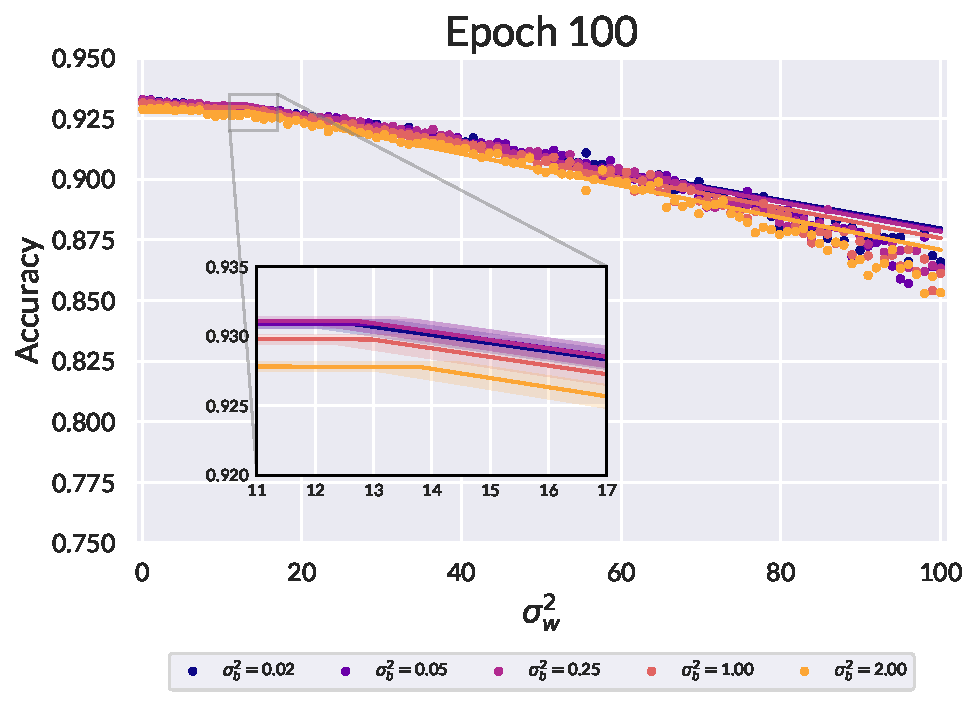
\includegraphics[width=\textwidth]{figures/chapter4/shallowNetworkSlope.pdf}
	\end{subfigure}%
	\begin{subfigure}[t]{0.5\textwidth}
		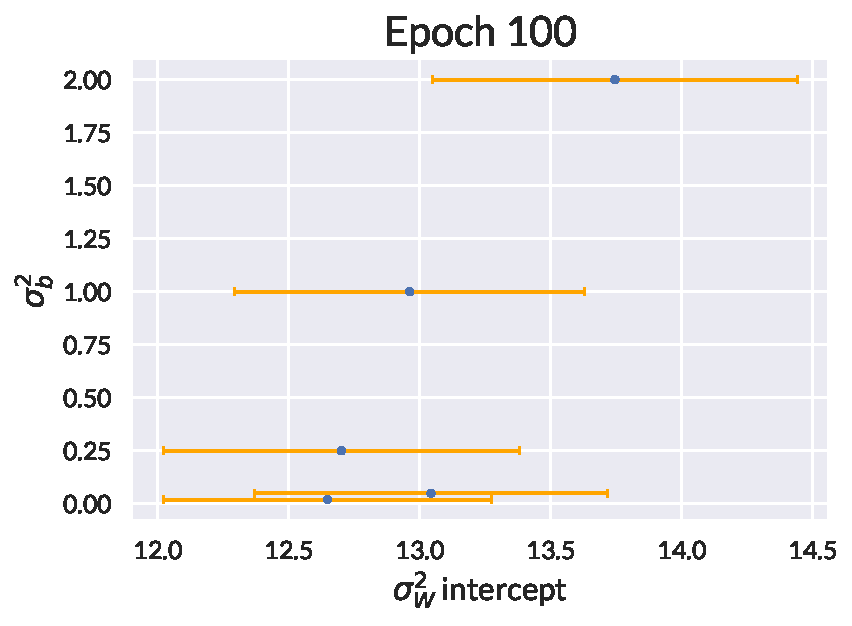
\includegraphics[width=\textwidth]{figures/chapter4/shallowNetworkSlopeIntercept.pdf}
	\end{subfigure}
	\caption{For small networks, the learning efficiency exhibits threshold behavior as a function of $\sigma_w^2$. Shown are results for MNIST trained on a $N=8$, $L=1$ network sampled over 50 network initializations. The inset shows the fits in the threshold region. The bottom figure shows that the location of this threshold in $\sigma_{w}^{2}$ decreases with increasing $\sigma_b^2$ consistent with the trend implied by the line of uniformity threshold. As explained in the text, there is a multiplicative factor involved and the large-$N$ analysis cannot be straightforwardly transplanted to this small-$N$ case. The uncertainty bars are propagated from the uncertainties in the accuracy versus $\sigma_{w}^{2}$ data points.}
	\label{fig:LOU-threshold}
\end{figure}

The effect of lying near uniformity is therefore strongest in shallow, narrow networks rather than deep, wide networks where the edge of chaos effect dominates. For these small networks, some of the asymptotic analysis above locating the LOU and EOC does not immediately apply, since the network is unable to reach the asymptotic value $\sigma_{*}^{2}$ of the pre-activation variance.\footnote{In this sense, we may take ``shallow'' to mean $L \leq 5$, since as shown in fig. \ref{fig:postevol}, by $L \approx 6$, the network has reached $\sigma_{*}^{2}$. Strictly speaking however, the predictions for the EOC as well as the LOU are ill-defined in narrow networks, since these are no longer approximately Gaussian, and also appear to be beyond the reach of current perturbative approaches \cite{Grosvenor:2021eol}.} At the same time, the input variance and mean, $\sigma_{0}^{2}$ and $\mu_0$, actually \emph{do} matter in this case and, with this information, we can roughly estimate the location of the line of uniformity. For example, for $L=1$, we have $\sigma_{1}^{2} = \sigma_{w}^{2} ( \sigma_{0}^{2} + \mu_{0}^{2} ) + \sigma_{b}^{2}$ and the line of uniformity would be where $\sigma_{1}^{2} = \sigma_{{\rm min}}^{2} = \frac{\pi^2}{12}$. For example, for MNIST, $\sigma_0^2 \approx 0.095$ and $\mu_{0}^{2} \approx 0.017$, so the line of uniformity can be estimated as $\sigma_b^2 \approx \frac{\pi^2}{12} - 0.112 \sigma_w^2$. Equivalently, for fixed $\sigma_b^2$, this gives a $\sigma_{w}^{2}$-threshold of $\sigma_w^2 \sim 7.35 + 8.93 \sigma_b^2$ beyond which we expect saturation effects to decrease training efficiency. For $L=2$, we would iterate the above process once more, passing through the activation function; this gives an estimated threshold of $\sigma_{w}^{2} \approx 3.5 +8.93\sigma_b^2 $. 

Results for $L=1$ are shown in fig. \ref{fig:LOU-threshold}, and results for $L=2$ are shown in fig. \ref{fig:LOU-threshold_L2}. As predicted, we observe that the accuracy retains a high, approximately constant value up to a $\sigma_b^2$-dependent threshold for $\sigma_w^2$, and then decays approximately linearly thereafter. To determine the threshold empirically, we fit the data to a function of the form
%
\begin{equation}
	A_{{\rm fit}} ( \sigma_{w}^{2} ) = A_{{\rm max}} - r ( \sigma_{w}^{2} - \sigma_{w, \text{thr}}^{2} ) \, \Theta ( \sigma_{w}^{2} - \sigma_{w, \text{thr}}^{2} ),
\end{equation}
%
where $A_{{\rm max}}$ is the maximum accuracy, $\sigma_{w, \text{thr}}^{2}$ is the threshold value, $r$ is the rate of linear decay, and $\Theta$ is the Heaviside step function. Each accuracy vs. $\sigma_{w}^{2}$ data point is an average over 20 instantiations of the network and thus comes with its own variance. These propagate into uncertainty bars for the three fit parameters. We plot the threshold for different values of $\sigma_{b}^{2}$ in fig. \ref{fig:LOU-threshold} for $L=1$. This qualitatively confirms our expectations, though the empirical value of the threshold is about a factor of 2 greater than the analytical prediction, and the slope about a factor of 8 smaller. However, given that we are applying a large-$N$ analysis to a relatively narrow network ($N=8$), an $\mathcal{O}(1)$ quantitative discrepancy is reasonable. For $L=2$ the corresponding results are presented in 
fig. \ref{fig:LOU-threshold_L2}, again showing qualitative agreement. The empirical threshold in this case is about a factor of 4 greater than the theoretical value, and the slope is a factor of $8$ smaller.

\begin{figure}[H]
	\centering
	\begin{subfigure}[t]{0.5\textwidth}
		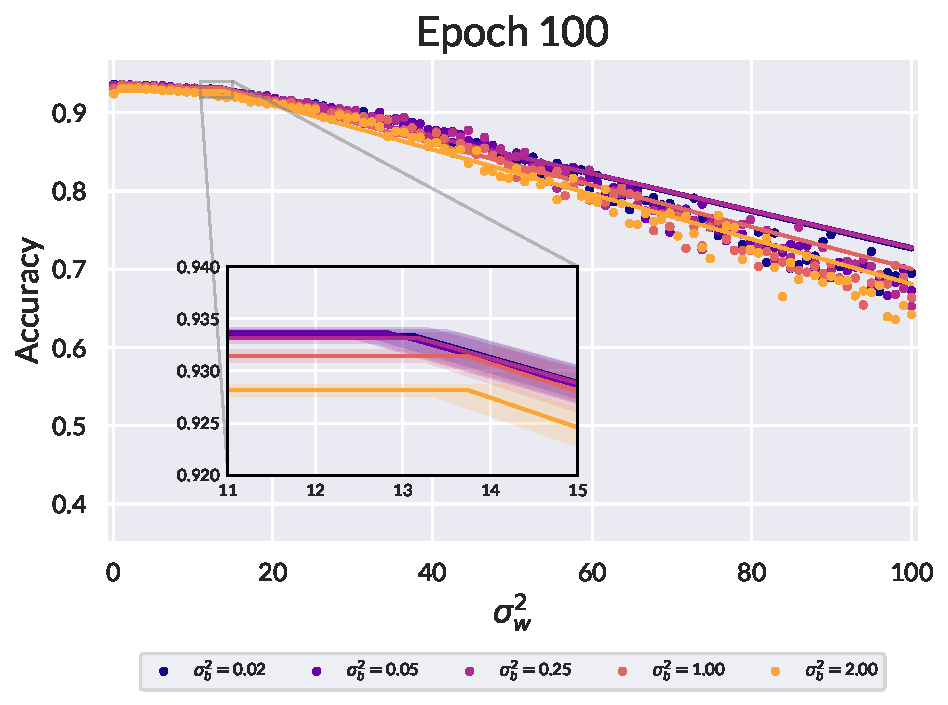
\includegraphics[width=\textwidth]{figures/chapter4/shallowNetworkSlopeL2.pdf}
	\end{subfigure}\hfill
	\begin{subfigure}[t]{0.5\textwidth}
		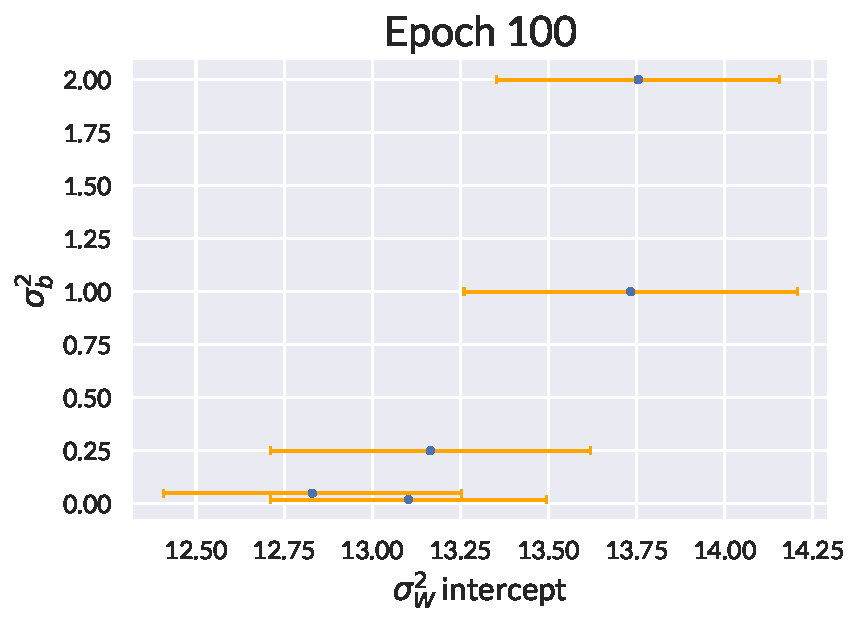
\includegraphics[width=\textwidth]{figures/chapter4/shallowNetworkSlopeInterceptL2.pdf}
	\end{subfigure}
	\caption{Small-network threshold behavior as in fig. \ref{fig:LOU-threshold}, for MNIST trained on a network with $N=8$ and $L=2$, sampled over 50 initial conditions drawn from $(\sigma_w^2,\sigma_b^2)$. The bottom figure shows that the location of this threshold decreases with $\sigma_b^2$ consistent with the trend implied by the line of uniformity.}
	\label{fig:LOU-threshold_L2}
\end{figure}

\emph{Conclusion} 
In this work, we establish that for deep random feedforward networks along the edge of chaos, the efficiency of training via stochastic gradient descent still depends on non-saturation of the activation function. Similar points have been made previously in \cite{2018arXiv180508266H,pmlr-v97-hayou19a}, which compared the performance of difference activation functions initialized at one point on their respective edges of chaos. However, what we demonstrate for the tanh activation function is that not all points on the edge of chaos are equally efficient at learning. Within a fixed number of training epochs ($\sim 100$), activation function saturation eventually impedes learning if we push the weight and bias variances too far to the right of the line of uniformity, defined to be where the final layer post-activation is most uniformly distributed, i.e., maximally entropic. Unlike the edge of chaos, which separates chaotic and ordered outputs, the line of uniformity does not mark an abrupt change in the overall behavior of the network. Rather, it simply indicates roughly the point where the saturation of the activation function begins to impede learning. We demonstrate this for shallow and narrow networks as well, where the exponential damping of neuron correlations away from the edge of chaos becomes much less of a decisive factor in determining training efficiency.

\section*{Acknowledgments}
This research was supported 
in part by the Dutch Research Council
(NWO) project 680-91-116 ({\em Planckian Dissipation and Quantum Thermalisation: From
	Black Hole Answers to Strange Metal Questions.}) and
by the Dutch Research
Council (NWO)/Ministry of Education. K.T.G. has received funding from the European Union’s Horizon 2020 research and innovation programme under the Marie Sk\l odowska-Curie grant agreement No 101024967.

\newpage
\section{Appendix}
\subsection{Independence of \texorpdfstring{$\sigma_{*}^{2}$}{sigmastarsquared} on \texorpdfstring{$\sigma_{1}^{2}$}{sigmaonesquared}}
\label{app:postevol}

The exact pre- or post-activation distribution at a given layer obviously does depend on $\sigma_{1}^{2}$, the pre-activation variance at the first hidden layer. This dependence is generated via the recursion relation \eqref{eq:varrecursion}. However, at the fixed point, the asymptotic distributions do not depend on $\sigma_{1}^{2}$. Indeed, the relation that the asymptotic pre-activation variance satisfies is eq. \eqref{eq:sigmastar}, which does not depend on $\sigma_{1}^{2}$ at all. We can demonstrate this fact by plotting the evolution of the post-activation distribution for fixed $\sigma_{w}^{2}$ and $\sigma_{b}^{2}$, but for many values of $\sigma_{1}^{2}$. In fig. \ref{fig:postevol}, we show this for $( \sigma_{w}^{2} , \sigma_{b}^{2} ) = (1.76, 0.05)$ for several values of $\sigma_{1}^{2}$, both less than and greater than $\sigma_{*}^{2}$ which turns out to be $\sigma_{*}^{2} \approx 0.57$ in this case. When $\sigma_{1}^{2} < \sigma_{*}^{2}$, the post-activation distribution starts out narrower and spreads out, whereas when $\sigma_{1}^{2} > \sigma_{*}^{2}$ it starts out more peaked at $\pm 1$ and then flattens out.
%
\begin{figure}[h!]
	\centering
	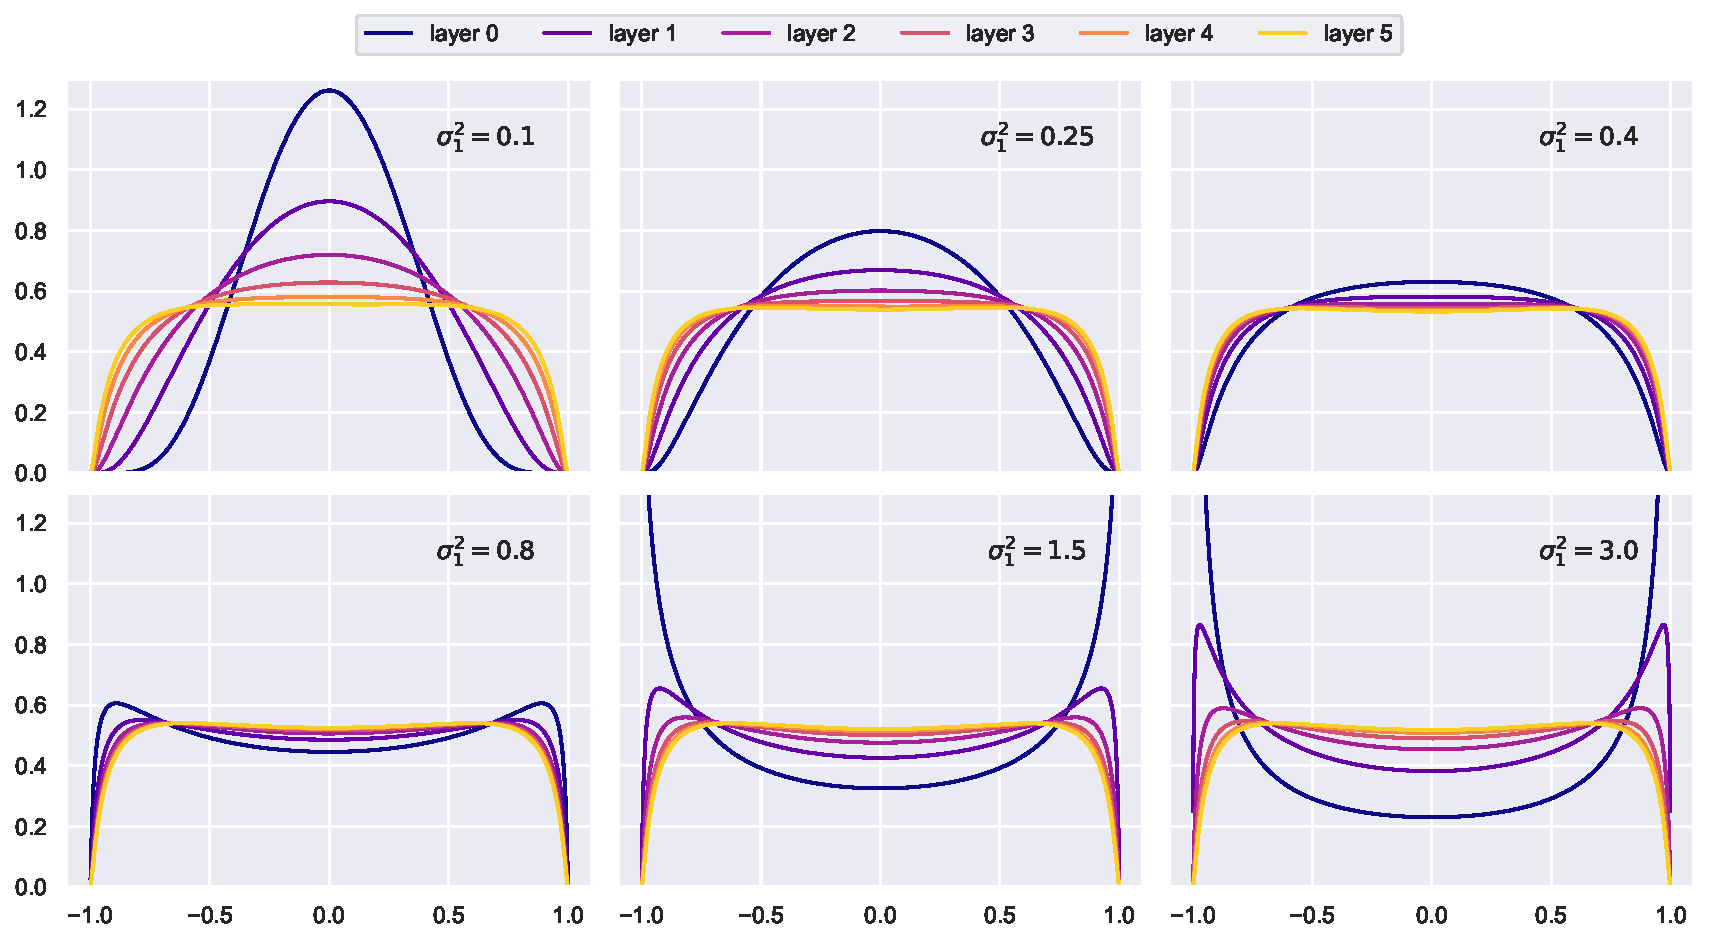
\includegraphics[width=\textwidth]{figures/chapter4/propagation_v2.pdf}
	\caption{Layer-to-layer evolution of the post-activation distribution at $( \sigma_{w}^{2} , \sigma_{b}^{2} ) = (1.76, 0.05)$ for six different values of the first hidden layer pre-activation variance $\sigma_{1}^{2}$. The post-activations converge to the asymptotic distribution within about five layers.}
	\label{fig:postevol}
\end{figure}

\subsection{Analytic Details of the Fixed Point Computation}
\label{app:analytics}

In this appendix, we will show that the edge of chaos contains the point $( \sigma_{w}^{2} , \sigma_{b}^{2} ) = (1,0)$ and has zero slope there. At this point, the fixed-point equation \eqref{eq:sigmastar} reads
%
\begin{equation}
	\sigma_{*}^{2} = \sigma_{\phi , *}^{2}~. 
\end{equation}
%
The left-hand side is the fixed-point pre-activation variance, whereas the right-hand side is the corresponding post-activation variance. As long as $| \phi (z) | < |z|$, which is the case for $\phi (z) = \tanh (z)$ except at $z=0$, the variance of the post-activation will always be smaller than that of the pre-activation. Therefore, the only solution at this point is $\sigma_{*}^{2} = \sigma_{\phi, *}^{2} = 0$ and thus at this point $\phi' ( \sigma_* z ) = \sech^2 (0) = 1$ and $\chi = 1$ or $\xi = \infty$. Hence, this point is on the edge of chaos.

Now, consider eq. \eqref{eq:fixedsigmastar}, but now along the edge of chaos rather than the lines of constant $\sigma_{*}^{2}$. Let $\sigma_{w}^{2}$ be our independent parameter along the edge of chaos and take a derivative with respect to it:
%
\begin{equation} \label{eq:derrel}
	\frac{\partial \sigma_{b}^{2}}{\partial \sigma_{w}^{2}} = \biggl( 1 - \sigma_{w}^{2} \, \frac{\partial \sigma_{\phi , *}^{2}}{\partial \sigma_{*}^{2}} \biggr) \frac{\partial \sigma_{*}^{2}}{\partial \sigma_{w}^{2}} - \sigma_{\phi , *}^{2}~,
\end{equation}
%
where we have used the fact that $\sigma_{\phi , *}^{2}$ depends on $\sigma_{w}^{2}$ only through its dependence on $\sigma_{*}^{2}$.

To compute the derivative $\frac{\partial \sigma_{\phi , *}^{2}}{\partial \sigma_{*}^{2}}$, it is convenient to first rewrite the integral expression for $\sigma_{\phi}^{2}$ in \eqref{eq:varpost} by changing back to the original pre-activation variable $z$:
%
\begin{align}
	\sigma_{\phi}^{2} = \int_{-1}^{1} \mathrm{d} x \, p_{\phi} ( x ; \sigma^2 ) \, x^2 = \int_{- \infty}^{\infty}\mathrm{d} z \, p(z ; \sigma^2 ) \, \phi (z)^2~.
\end{align}
%
We can easily compute the various derivatives of the pre-activation distribution:
%
\begin{align}
	\frac{\partial p(z ; \sigma^2 )}{\partial \sigma^2} &= \biggl( \frac{z^2}{\sigma^2} -1 \biggr) \frac{p(z ; \sigma^2 )}{2 \sigma^2}, &%
	%
	\frac{\partial^2 p(z; \sigma^2 )}{\partial z^2} &= \biggl( \frac{z^2}{\sigma^2} -1 \biggr) \frac{p(z ; \sigma^2 )}{\sigma^2} = 2 \, \frac{\partial p(z ; \sigma^2 )}{\partial \sigma^2}~.
\end{align}
%
Therefore, using integration by parts, and the fact that we can ignore boundary terms due to the fast fall-off of the Gaussian, we find
%
\begin{align} \label{eq:paderiv}
	\frac{\partial \sigma_{\phi}^{2}}{\partial \sigma^2} = \int \mathrm{d} z \, \frac{\partial p (z ; \sigma^2)}{\partial \sigma^2} \, \phi (z)^2 = \frac{1}{2} \int \mathrm{d} z \, \frac{\partial^2 p(z ; \sigma^2 )}{\partial z^2} \, \phi (z)^2 = \int \mathrm{d} z \, p(z ; \sigma^2 ) \bigl( \phi' (z)^2 + \phi(z) \, \phi'' (z) \bigr)~.
\end{align}
%
By rescaling the variable to $\sigma z$, the first integral term above can be written as
%
\begin{equation}
	\int \mathrm{d} z \, p(z; \sigma^2 ) \phi' (z)^2 = \int \mathcal{D} z \, \bigl[ \phi' ( \sigma z ) \bigr]^2~.
\end{equation}
%
Note that when this is evaluated at $\sigma_{*}^{2}$ and multiplied by $\sigma_{w}^{2}$, we get precisely $\chi$, as defined in \eqref{eq:corlength}. Let us give a name to the remaining integral in \eqref{eq:paderiv} evaluated at $\sigma_{*}^{2}$. For future convenience, we will put a relative minus sign in the definition below, the reason being that, for $\phi = \tanh$, the object $\phi \, \phi''$ is \emph{negative} semi-definite:
%
\begin{equation}
	\tilde{\chi} = - \sigma_{w}^{2} \int \mathrm{d} z \, p (z ; \sigma_{*}^{2} ) \, \phi (z) \, \phi '' (z) = - \sigma_{w}^{2} \int \mathcal{D} z \, \phi ( \sigma_* z ) \, \phi '' ( \sigma_* z )~.
\end{equation}
%
Then, \eqref{eq:paderiv} evaluated at $\sigma_{*}^{2}$ and multiplied by $\sigma_{w}^{2}$ reads
%
\begin{equation} \label{eq:paderiv2}
	\sigma_{2}^{2} \frac{\partial \sigma_{\phi , *}^{2}}{\partial \sigma_{*}^{2}} = \chi - \tilde{\chi}~.
\end{equation}
%
Now, let us define
%
\begin{equation}
	\tilde{\xi} = - \frac{1}{\ln ( \chi - \tilde{\chi} )}~.
\end{equation}
%
This is precisely the object called $\xi_q$ in \cite{2016arXiv161101232S}, which is the length scale that controls the exponential decay of information propagation through the neural network from a single input.

Plugging eq. \eqref{eq:paderiv2} back into eq. \eqref{eq:derrel} gives
%
\begin{align}
	\frac{\partial \sigma_{b}^{2}}{\partial \sigma_{w}^{2}} = ( 1 - \chi + \tilde{\chi} ) \frac{\partial \sigma_{*}^{2}}{\partial \sigma_{w}^{2}} - \sigma_{\phi , *}^{2}~.
\end{align}
%
Along the edge of chaos, $\chi = 1$, and so
%
\begin{align} \label{eq:derrel1}
	\frac{\partial \sigma_{b}^{2}}{\partial \sigma_{w}^{2}} = \tilde{\chi} \frac{\partial \sigma_{*}^{2}}{\partial \sigma_{w}^{2}} - \sigma_{\phi , *}^{2}~,
\end{align}
%
Now, we can establish a simple bound on $\tilde{\chi}$ by virtue of the fact that $|\phi (z) | \leq |z|$, for $\phi = \tanh$. To do this, let us first rewrite $\tilde{\chi}$ using the identity
%
\begin{equation}
	\phi'' (z) = - 2 \tanh(z) \sech^2 (z) = -2 \, \phi (z) \, \phi'(z)~.
\end{equation}
%
Therefore,
%
\begin{equation}
	\phi (z) \, \phi'' (z) = - 2 \, \phi (z)^2 \, \phi' (z) = - \frac{2}{3} \bigl[ \phi (z)^3 \bigr]'~,
\end{equation}
%
and
%
\begin{equation}
	\tilde{\chi} = \frac{2 \sigma_{2}^{2}}{3} \int \mathrm{d} z \, p(z ; \sigma_{*}^{2} ) \bigl[ \phi (z)^3 \bigr]' = - \frac{2 \sigma_{w}^{2}}{3} \int \mathrm{d} z \, \frac{\partial p(z ; \sigma_{*}^{2} )}{\partial z} \, \phi (z)^3 = \frac{2 \sigma_{w}^{2}}{3 \sigma_{*}^{2}} \int \mathrm{d} z \, p (z ; \sigma_{*}^{2} ) \, z \, \phi (z)^3~.
\end{equation}
%
Therefore, since $|\phi (z) | \leq |z|$ for $\phi = \tanh$,
%
\begin{align}
	0 \leq \tilde{\chi} \leq \frac{2 \sigma_{w}^{2}}{3 \sigma_{*}^{2}} \int \mathrm{d} z \, p ( z; \sigma_{*}^{2} ) \, z^4 = 2 \, \sigma_{w}^{2} \, \sigma_{*}^{2}~.
\end{align}
%
Therefore, since we have already shown that $\sigma_{*}^{2} = \sigma_{\phi , *}^{2} = 0$ at the point $( \sigma_{w}^{2} , \sigma_{b}^{2} ) = (1,0)$, it follows that $\tilde{\chi} = 0$ at this point as well and, from eq. \eqref{eq:derrel1},
%
\begin{equation}
	\frac{\partial \sigma_{b}^{2}}{\partial \sigma_{w}^{2}} \biggr|_{( \sigma_{w}^{2} , \sigma_{b}^{2} ) = (1,0)} = 0~.
\end{equation}
%
In other words, the edge of chaos has zero slope at the point $( \sigma_{w}^{2} , \sigma_{b}^{2} ) = (1,0)$.

\subsection{Implementation Details}
\label{app:figs}

Throughout this work, we have used a vanilla feedforward neural network of $L$ hidden layers, each having the same depth $N$. As described, initial weights and biases are drawn from zero-mean Gaussian distributions with $\frac{\sigma_w^2}{N}$ and $\sigma_b^2$ respectively. Both MNIST and CIFAR-10 were trained using the standard cross-entropy loss function and no optimizer. This reproduces the results of \cite{2016arXiv161101232S} (see fig. \ref{fig:googleBrain-repro}), confirming critical behavior.
\begin{figure}[H]
	\centering
	\includegraphics[scale=.9]{figures/chapter4/googleGraph.pdf}
	\caption{Optimal learning for deep neural networks at the edge of chaos as first shown by \cite{2016arXiv161101232S}. Shown is learning efficiency for MNIST training as a function of network depth $L$ with $N=784$ and choice of initial weight distribution $\sigma_w^2$ holding the initial bias distribution $\sigma_b^2=0.05$ fixed. At the edge of chaos $(\sigma_w^2,\sigma_b^2)=(1.76,0.05)$, learning remains efficient even for very deep networks, but eventually ($L\sim 270$) goes down. This same behavior has been observed for deep feedforward networks in \cite{2016arXiv161101232S,Erdmenger:2021sot}. The learning rate used is $\ell = 10^{-3}$ for $L<100$ and $\ell=10^{-4}$ for $L\geq100$.}
	\label{fig:googleBrain-repro}
\end{figure}

\subsection{SWISH activation function}\label{app:swish}

Throughout the text, we examined the impact of saturation via the line of uniformity for the tanh activation function. For non-saturating activation functions, it is an open question whether a similar notion of uniformity exists. While a full analysis of this is beyond the scope of this work, in this appendix we offer some preliminary results for the SWISH activation function,
\begin{equation}
	\mathrm{swish}(z)=\frac{z}{1+e^{-z}}~,
\end{equation}
which also features a line of critical points separating an ordered and chaotic phase. Note that unlike the EOC for tanh, which increases with increasing $\sigma_w^2$, the EOC for SWISH decreases with increasing $\sigma_w^2$, which prevents us from examining the impact of large weight variances. Conversely, for small values of $\sigma_w^2$, the corresponding value of $\sigma_b^2$ becomes so large that we are unable to satisfy the critical detection criteria $\chi=1$ discussed in the main text.\footnote{We do not claim that the EOC stops beyond this point, rather that it cannot be computed from the central limit method used in \cite{arxiv.1606.05340, 2016arXiv161101232S}. It is conceivable that this could be computed via the NN/QFT correspondence developed in \cite{Grosvenor:2021eol}, but this has not been attempted for SWISH.} The EOC for SWISH is plotted in fig. \ref{fig:swisheoc}, which shows a computable range of approximately $\sigma_w^2\in[1.97,3.4]$. The same figure also shows the accuracy for an $L=40$ network with SWISH activation function trained along the EOC, demonstrating no deterioration of performance within this range, which confirms the absence of saturation effects. See also \cite{2018arXiv180508266H,pmlr-v97-hayou19a}.

\begin{figure*}[h!]
	\centering
	\begin{subfigure}{0.5\textwidth}
		\centering
		\includegraphics[width=\linewidth]{figures/chapter4/SwishEOC.pdf}
	\end{subfigure}%
	\begin{subfigure}{0.5\textwidth}
		\centering
		\includegraphics[width=\linewidth]{figures/chapter4/Swish_accuracy.pdf}
	\end{subfigure}
	\caption{(Left) Edge of chaos for SWISH activation function. (Right) Accuracy for a feedforward network with $L=40$ layers trained on MNIST for 21 equally-spaced points along the SWISH EOC. Over the limited range for which the criticality condition $\chi=1$ is satisfied, we observe no significant differences in accuracy, though a slightly lower learning rate was used for the left-most two points; we believe this to be due to the large values of $\sigma_b^2$ in this regime. \label{fig:swisheoc}}
\end{figure*}


		
		\thumbfalse
		
		\addcontentsline{toc}{part}{References}
		\setheader{References}
		
		
		\bibliographystyle{JHEP}
		{\bibliography{library}}
		
		
		%\newpage
\thispagestyle{empty}

\chapter*{Samenvatting}
\addcontentsline{toc}{part}{Samenvatting}
\setheader{Samenvatting}
\label{Samenvatting}


Vaste stoffen bestaan uit elektronen en ionen. De meeste vaste stoffen kunnen effectief worden gemodelleerd met een theorie waarin de beweging van de elektronen allemaal als onafhankelijk van elkaar kan worden beschouwd. Dit proefschrift houdt zich bezig met enkele gevallen waarin deze beschrijving onvermijdelijk faalt, en veel-deeltjes-interacties de lage-energiefysica domineren. Dergelijke systemen zijn veel moeilijker te bestuderen, en soms kan vooruitgang worden geboekt met behulp van geavanceerde numerieke technieken, of door creatief geconstrueerde, precies oplosbare speelgoedmodellen.
\par
Dit laatste is de benadering van het Sachdev-Ye-Kitaev (SYK)-model, dat een kwantumdot beschrijft met een groot aantal fermionen erop, die allemaal met elkaar interacteren door middel van een gerandomiseerde interactie met vier fermionen. De eenvoud van het model verhult een overvloed aan exotische verschijnselen die voortkomen uit een emergente conforme symmetrie in het infrarood, met eclectische toepassingen van vreemde metalen tot zwarte gaten. Door de holografische dualiteit kan de lage-energietheorie van het model, die voortkomt uit het verbreken van de bovengenoemde conforme symmetrie, in kaart worden gebracht op verstoringen van een bijna AdS${}_2$ ruimtetijd. 
\par
Eén van die verschijnselen staat bekend als maximale chaos. Het SYK-model verzadigt een grens aan de snelheid waarmee een kwantumsysteem verstoringen kan dissiperen in zijn vrijheidsgraden. Dit kenmerk blijft bestaan, zelfs als men bepaalde gewijzigde versies van het SYK-model construeert, zoals het bipartiete SYK-model, en de mate van chaos verandert niet, zelfs niet als de schaaldimensies van de samenstellende fermionen worden veranderd, zoals beschreven in hoofdstuk ~\ref {ch:LyapbSYK}. De eerste subleidraad voor conforme correctie van de chaos-exponent blijkt ook onafhankelijk te zijn van de schaaldimensie.
\par
Wanneer twee identieke kopieën van het SYK-model aan elkaar worden gekoppeld door een tunnelinteractie, beschrijft het holografische duaal de ruimtetijd van een wormgat bij lage temperatuur. Een op een dergelijke manier gemaakt Josephson-contact kan worden bestudeerd met behulp van de SYK-versie van het elektron-fonon-gekoppelde systeem, dat bekend staat als het Yukawa SYK-model. Supergeleiding in het Yukawa SYK-model vindt plaats bij het herstel van de tijdomkeersymmetrie bij lage temperaturen. In hoofdstuk~\ref{chap:JosephsonWormhole} werd aangetoond dat de niet-supergeleidende toestand de correcte niet-analytische afhankelijkheid van de kloof vertoont van de sterkte van de tunnelinteractie, kenmerkend voor de wormgattoestand. Er werd aangetoond dat de supergeleidende toestand effectief kan worden beschreven door een twee-vloeistoffenmodel, waarbij de Cooperparen onafhankelijk aan beide zijden leven, terwijl excitaties van enkele elektronen nog steeds de wormgattoestand vormen.
\par
Afwijkend van de hyperbolische geometrie van de AdS${}_2$ ruimte, hebben we in het tweede deel van dit proefschrift een systeem beschouwd waarvan het niet-interagerende fermi-oppervlak was samengesteld uit een familie van hyperbolen. In gedraaid dubbellaags grafeen voor kleine draaihoeken is dit te zien in de vorm van van Hove-singulariteiten, die precies onder de magische hoek een hogere orde krijgen. In hoofdstuk~\ref{ch:KondoTBG} werd aangetoond dat een sonde voor het waarnemen van het effect ervan in een realistische fysieke omgeving een reactie is op een magnetische onzuiverheid. De onzuiverheidsentropie vertoont duidelijke kenmerken nabij de magische hoek, en toont stromingen naar de verschillende soorten vaste punten die beschikbaar zijn in de faseruimte van het systeem. Totdat de magische hoek is bereikt, werkt het bestaan van de Dirac-kegel bij de laagste energieën als een afschrikmiddel voor Kondo-screening, wat zich manifesteert als een entropie van $\log 2$ per onzuiverheid. In de magische hoek domineert de verschijning van de hogere orde Van Hove-singulariteit de bandstructuur, en dit leidt tot een versterkt Kondo-effect tot de laagst mogelijke energieschalen.

\newpage
\thispagestyle{empty}
		%\newpage
\thispagestyle{empty}

\chapter*{Summary}
\addcontentsline{toc}{part}{Summary}
\setheader{Summary}
\label{Summary}

Solids are composed of electrons and ions. Many solids can be effectively modeled by considering a free electron theory. This thesis is concerned with some cases where that description inevitably fails, and many body interactions dominate the low energy physics. Such systems are far more difficult to study, and sometimes progress can be made either with sophisticated numerical tools, or by creatively constructed exactly solvable toy models.
\par
The latter is the approach taken by the Sachdev-Ye-Kitaev (SYK) model, which describes a quantum dot with a large number of fermions on it, all interacting with each other by means of a randomized four-fermion interaction. The simplicity of the model belies a plethora of exotic phenomena that arise from an emergent conformal symmetry in the infrared, with eclectic applications from strange metals to black holes. Through the holographic duality, the low energy theory of the model arising from the breaking of the aforementioned conformal symmetry can be mapped to perturbations of a nearly AdS${}_2$ spacetime. 
\par
One such phenomenon is known as maximal chaos. The SYK model saturates a bound on the rate at which a quantum system can dissipate perturbations into its degrees of freedom. This feature persists even when one constructs certain modified versions of the SYK model, such as the bipartite SYK model, and the rate of chaos doesn't change even when the scaling dimensions of the constituent fermions are changed as is described in chapter~\ref{ch:LyapbSYK}. The first subleading to conformal correction to the chaos exponent is also found to be independent of the scaling dimension. 
\par
When two identical copies of the SYK model are coupled together by a tunneling interaction, its holographic dual describes a wormhole spacetime at low temperature. A Josephson contact made in such a way can be studied using the SYK version of the electron-phonon coupled system, which is known as the Yukawa SYK model. Superconductivity in the Yukawa SYK model occurs upon on the restoration of time reversal symmetry at low temperatures. In chapter~\ref{chap:JosephsonWormhole}, it was shown that the non-superconducting state shows the correct non-analytic dependence of the gap on the strength of the tunneling interaction, characteristic of the wormhole state. The superconducting state was shown to be effectively described by a two-fluid model, where the cooper pairs live independently on the two sides, while single electron excitations still form the wormhole state. 
\par
Departing from the hyperbolic geometry of the AdS${}_2$ space, we considered a system whose non-interacting fermi surface was composed of a family of hyperbolae in the second part of this thesis. In Twisted bilayer graphene for small twists, this is seen in the form of van Hove singularities, which turn higher order at precisely the magic angle. In chapter~\ref{ch:KondoTBG}, a probe for sensing its effect in a realistic physical setting was shown to be the in response of a magnetic impurity. The impurity entropy shows distinct signatures near the magic angle, showing flows to the different kinds of fixed points available in the phase space of the system. Until the magic angle is reached, the existence of the Dirac cone at the lowest energies acts as a deterrent for Kondo screening, which manifests itself as a $\log 2$ entropy per impurity. At the magic angle however, the appearance of the higher order van Hove singularity dominates the band structure, and it leads to an enhanced Kondo effect until the lowest energy scales possible.


%perhaps turn the following off if the summary lasts two pages
\newpage
\thispagestyle{empty}
		%\newpage
\thispagestyle{empty}

\chapter*{List of Publications}
\addcontentsline{toc}{part}{List of Publications}
\setheader{List of Publications}
\label{publications}

\begin{enumerate}[leftmargin=*]
\setlength{\itemsep}{15pt}

    \item   `` New approaches for boosting to uniformity'',
    
         A. Rogozhnikov, \textbf{A. Bukva}, V. Gligorov, A. Ustyuzhanin and M. Williams  \\
         \textit{JINST}, 11 (2015) T03002. 

         
    \item ``Operator thermalization vs eigenstate thermalization'',
    
            \textbf{A. Bukva},  Philippe Sabella-Garnier, Koenraad Schalm, \\
            e-Print: 1911.06292. 

            
    \item ``Criticality versus uniformity in deep neural networks'',

            \textbf{Aleksandar Bukva}, Jurriaan de Gier, Kevin T. Grosvenor, Ro Jefferson, Koenraad Schalm, Eliot Schwander \\
            e-Print: 2304.04784, submitted to \textit{JMLR}.

    \item ``Replicating Higgs fields in Ising gauge theory: the registry order'',

           \textbf{Aleksandar Bukva}, Koenraad Schalm, Jan Zaanen  \\
           e-Print: 2305.02400, submitted to \textit{Phys.Rev.E}.
\end{enumerate}


\newpage
\thispagestyle{empty}
		%\newpage
\thispagestyle{empty}

\chapter*{Curriculum Vitae} %important is to use the * after chapter. This way there is not an extra chapter nummer added to these sections
\addcontentsline{toc}{part}{Curriculum Vitae}
\setheader{Curriculum Vitae}
\label{Curriculum Vitae}

I was born on September 26th, 1996 in Chennai, a big city in the south of India. After finishing high school, I went to West Bengal for a five-year integrated Bachelor-Master program in Physics at the Indian Indian Institute of Technology, Kharagpur.
\par
High school was the place where I discovered that I wanted to study physics later in life. Besides the regular high school curriculum, I attended the physics seminar at Petnica science center. I was quickly introduced to the world of computer simulations and developed a particle-in-cell (PIC) code for simulating a plasma wave accelerator. After finishing high school, I moved to Belgrade, where I obtained my bachelor's degree. In the first year, my publication ``New Approaches for Boosting to Uniformity'' was awarded the best technical paper at Belgrade University. During my bachelor's, I continued my interest in computational physics. I did a summer internship at Helmholtz-Zentrum Dresden Rossendorf in a group of Dr. Michael Bussmann, where I worked on an improved version of an integration algorithm for their PIC code. 
\par
I continued my master's degree in Belgrade. Still, I did most of my thesis work at the Institute of Physics under the supervision of Milica Milovanović. The title of my master's thesis is: ``Lattice-like structures in Lowest Landau Level'' where we were trying to construct an effective Hamiltonian for a bosonic system on a square lattice that will support fractional quantum Hall effect (FQHE) at $\nu=\frac{1}{2}$. I started my Ph.D. in November 2018, in the Quantum Matter Theory Group at the Lorentz Institute of Leiden University, under the supervision of Prof. Dr. J. Zaanen and Prof. Dr. K.E. Schalm. During my Ph.D., I taught a couple of courses as a teaching assistant, ``Classical Electrodynamics'' and ``Theory of General Relativity''. Alongside the research, I have attended several schools during my Ph.D., DRSTP Schools in High Energy and Condensed Matter Physics, in Brazil and the Netherlands. I have also presented my work at several Physics@Veldhoven conferences.

As of January 1st, 2023, I have started working as a Quantitative Developer for an energy trading company Northpool B.V.


\newpage
\thispagestyle{empty}
		%\newpage
\thispagestyle{empty}

\chapter*{Acknowledgements}
\addcontentsline{toc}{part}{Acknowledgements}
\setheader{Acknowledgements}
\label{Acknowledgements}

First and foremost, I would like to thank my promotors Prof. Vadim Cheianov and Prof. Koenraad Schalm for giving me the independence to carve my own path, even though it might have been slightly unconventional. I'm very thankful to Vadim for his infinite patience with my questions and for addressing them sincerely even if they might have been trivial at times. To Koenraad I'm thankful for teaching me to improve my scientific rigor and for the importance he taught me to place on communicating my results well. Thank you very much. 
\par
I'm most greatly indebted to Prof. Lars Fritz, his contribution to this work goes far beyond his supervision of the two published papers that form parts of this thesis. I'm exceedingly grateful to him for welcoming me into his group, and for his wonderful mentorship over the years. I'm also thankful to Lars for introducing me to Prof. Andrew K. Mitchell, who I greatly enjoyed collaborating with. I hope this collaboration will last for quite some time to come. 
\par
I'm also very grateful to the PhD students and postdocs that I worked with in Leiden and in Utrecht - Dima Oriekhov, Mikael Fremling and Stephan Plugge. I am also particularly grateful to the several intense discussions I had with Nicolas Chagnet over physics and on numerics in general. I would also like to acknowledge master students Alina Melissakis and Nina Doerfler whose theses I helped co-supervise- I learned quite a lot from this experience.
\par
I extend thanks next to the several friends I made along the way. I will always have a special place for my covid-housemate Alicja Dutkiewicz, and my post-covid housemate Dimitrios Krommydas, with whom I felt that family was always close by. 
\par
I also thank Floris Balm, Luca Barbera, Alexander Barnaveli, Norman Bluemel,  Meike Bos, Aleksandar Bukva, Zhenya Cheipesh, Jose Collado, Tjeerd de Leede, David Dechant, Emanuele di Salvio, Alvaro Donis-Vela, Patrick Emonts, Inci Erbilen, Matthias Flor, Ireth Garcia-Aguilar, Alice Garoffolo, Peter George, Joren Harms, Yaroslav Herasymenko, Ludwig Hoffman, Stef Koenis, Ilse Kuijf, Gal Lemut, Samadarshi Maity, Savvas Malikis, Simon Marshall, Kirsten Martens, Kamil Matuszelanski, Anna Negro, Vladimir Ohanesjan, Maialen Ortego-Larrazabal, Michal Pacholski, Adrian Perez, Stefano Polla, Kshiti Sneh Rai, Midas Ratsma, Philippe Sabella-Garnier, Katerina Saiti, Kolya Semenyakin, Tereza Vakhtel, Vova Zakharov and Masha Zakharova for their warm company, and for discussions both physics and otherwise. 
\par
I'm also very thankful to my friends from India - Mohit Chajjed, Mohit Dhariwal, Muthu Ganesh, Philip Jacob, Viraj Jangam, Daksh Khanter, Dilip Kumar, Pranai Kumar, Praveen PR, Saloni Priya, Suvrat Rao, Darvin Sai Teja Reddy, Baibhaw Kumar Singh, Tulja Varun for keeping me company with frequent phone calls, especially during the pandemic. 
\par
Lastly, I thank my family - Amma, Appa, Aparna and Paati-Thatha for your support, and for being understanding of my absence from home. 
\newpage
\thispagestyle{empty}
		
	\end{document}
